% !TeX program = xelatex
\documentclass[UTF8,a4paper,zihao=-4]{ctexart}

\usepackage{geometry}
\usepackage{graphicx}
\usepackage{array}
\usepackage{setspace}
\usepackage{titlesec}
\usepackage{hyperref}
\usepackage{float}
\usepackage{booktabs}
\usepackage{caption}
\usepackage{xcolor}
\usepackage{listings}

\geometry{left=2.6cm,right=2.6cm,top=2.4cm,bottom=2.4cm}
\setcounter{secnumdepth}{3}
\setcounter{tocdepth}{3}
\hypersetup{hidelinks}

\definecolor{codebg}{RGB}{248,248,248}
\definecolor{codeframe}{RGB}{180,180,180}
\lstset{
  backgroundcolor=\color{codebg},
  basicstyle=\ttfamily\footnotesize,
  breaklines=true,
  frame=single,
  framerule=0.4pt,
  rulecolor=\color{codeframe},
  numbers=left,
  numberstyle=\tiny\color{gray},
  stepnumber=1,
  tabsize=2,
  showstringspaces=false,
  columns=flexible,
  keepspaces=true,
  xleftmargin=1.8em,
  framexleftmargin=1.8em,
  aboveskip=0.6em,
  belowskip=0.6em,
}
\renewcommand{\lstlistingname}{代码清单}

\titleformat{\section}{\centering\zihao{3}\bfseries}{第\chinese{section}章}{1em}{}
\titleformat{\subsection}{\zihao{4}\bfseries}{\thesubsection}{1em}{}
\titleformat{\subsubsection}{\zihao{-4}\bfseries}{\thesubsubsection}{1em}{}

\newcommand{\coverline}[2]{%
  \makebox[3.2cm][l]{\zihao{4}#1}%
  \underline{\makebox[7.8cm][l]{\zihao{4}#2}}%
}
\newcommand{\reportfig}[4][0.92\textwidth]{%
  \begin{figure}[H]
    \centering
    \includegraphics[width=#1]{#2}
    \caption{#3}
    \label{#4}
  \end{figure}
}

\begin{document}

\begin{titlepage}
  \centering
  \vspace*{0.4cm}

  
\includegraphics[width=14.0cm]{assets/swjtu-title.png}

  \vspace{1.0cm}
  
\includegraphics[width=6.0cm]{assets/swjtu-logo.png}

  \vspace{1.3cm}
  {\zihao{2}\bfseries 云计算技术\par}

  \vspace{1.4cm}
  {\zihao{2}\bfseries 课程设计报告\par}

  \vfill

  \begin{minipage}{11.2cm}
    \setstretch{1.85}
    \coverline{专业年级：}{软件工程专业 2023级}\\
    \coverline{组员1：}{李欣纯（2023116052）}\\
    \coverline{组员2：}{郑瑞璟（2023115271）}\\
    \coverline{指导老师：}{丛荣}\\
    \coverline{提交日期：}{2026年5月21日}\\
  \end{minipage}

  \vspace*{1.0cm}
\end{titlepage}

\pagenumbering{Roman}
\tableofcontents
\newpage
\pagenumbering{arabic}

\section{课程设计概述}
\subsection{设计目标与任务要求}

本课程设计主要分为云计算平台搭建和并行编程实战两部分。项目在华为云环境中完成应用容器化、镜像推送、Kubernetes 集群部署、Spark 数据分析和性能对比等工作。与只在本地运行脚本不同，本项目需要把容器、Service、LoadBalancer、PVC、ConfigMap、HPA 和 Spark 作业放到真实 CCE 环境中验证，因此报告重点记录配置过程、截图证据和排错依据。

任务书将课程设计划分为“云计算平台搭建”和“并行编程实战”两项主体任务，并将报告质量作为独立评分内容。其中，第一部分满分 50 分，要求在华为云 CCE 上部署“Flask 后端 API + Redis 数据库”两层 Web 应用，并完成应用容器化、CCE 集群搭建、Kubernetes 应用部署、Redis 持久化存储、ConfigMap Volume 挂载以及 HPA 弹性伸缩验证。第二部分满分 40 分，要求在第一部分建立的 Kubernetes 平台上选择 Spark 大数据分析或 MPI 并行科学计算方向完成并行编程实践。本项目选择方向 A，即 Spark 大数据分析，并围绕数据清洗、Spark SQL 统计分析、性能对比和 Amdahl 定律分析展开。报告质量部分满分 10 分，重点考查结构完整性、截图清晰度、图表规范性和结果分析深度。

\subsubsection{总体设计目标}

本项目的目标是让 Web 应用和 Spark 分析任务都能在云端正常运行，并留下可以复验的截图和配置文件。在平台层面，后端服务、Redis 和前端静态页面分别构建为容器镜像，再通过 Kubernetes Deployment、Service、ConfigMap、Secret、PVC 和 HPA 完成部署。在数据计算层面，项目选择 Spark 大数据分析方向，利用 PySpark 对电影数据进行清洗、聚合统计、趋势分析和性能测试。

图 \ref{fig:overall-architecture} 给出了本项目的总体架构。在线应用链路以 ELB 和 \verb|backend-svc| 为公网请求入口，请求由 Service 转发至两个 Flask 后端副本，后端再通过集群内部的 \verb|redis-svc| 访问 Redis；Redis 数据目录由 PVC 提供持久化存储。Nginx 前端通过反向代理复用后端 Service，ConfigMap、Secret 与 HPA 分别承担配置注入、敏感信息管理和副本弹性调节。离线分析链路则由 Spark Operator 在同一 CCE 集群中调度 Driver 与 Executor，读取 OBS 或实验数据集并输出统计与性能分析结果。两条链路共享 Kubernetes 计算环境，但在服务入口、状态存储和任务调度方面保持职责分离。

\reportfig[\textwidth]{figures/course-architecture.png}{课程设计总体架构与关键数据流}{fig:overall-architecture}

从能力培养角度看，本课程设计旨在形成以下几方面的综合实践能力：第一，能够根据任务书模板修改 Dockerfile 和应用配置，完成本地构建、联调与镜像推送；第二，能够在华为云 CCE 中创建满足版本和节点数量要求的 Kubernetes 集群，并使用 kubectl 进行资源管理与状态核验；第三，能够合理使用 ConfigMap、Secret、PVC、LoadBalancer 和 HPA 等资源解决配置分离、敏感信息管理、数据可靠性、外部访问和弹性伸缩问题；第四，能够在 Kubernetes 环境中运行 Spark 作业，并使用 Spark DataFrame 与 SQL API 完成数据分析任务；第五，能够基于截图、日志、实验数据和理论模型对实验结果进行解释，而不是仅停留在操作记录层面。

\subsubsection{云计算平台搭建任务要求}

云计算平台搭建部分按照任务书 T1 至 T6 组织。T1 要求完成应用容器化：后端 Dockerfile 需保留多阶段构建结构，并在依赖文件中加入至少一个自选 Python 包；前端 Nginx 默认首页需包含本人学号和姓名；本地需通过 Docker Compose 验证后端与 Redis 通信正常，并将后端、前端镜像推送到 SWR，保留镜像名称和 Tag 的控制台截图。T2 要求通过 CCE 控制台创建 Kubernetes 集群，集群版本不低于 1.27，至少包含两个 Worker 节点，并通过 \verb|kubectl get nodes -o wide| 证明节点处于 Ready 状态且输出中包含 VERSION 列。

T3 要求将任务 1 形成的镜像部署到 CCE 集群。后端 Deployment 需设置两个副本，配置资源请求与限制，并通过 ConfigMap 注入 Redis 地址、通过 Secret 注入 Redis 密码；Redis Deployment 设置一个副本，并通过 ClusterIP Service 仅在集群内部访问；后端 Service 使用 LoadBalancer 类型并绑定华为云 ELB，使外部能够访问 \verb|/api/ping| 并获得正常 JSON 响应。T4 要求为 Redis 配置 PVC，并通过“写入数据、删除 Pod、重建后查询”的过程证明数据未丢失。T5 要求将 Nginx 反向代理配置以 ConfigMap Volume 形式挂载到前端 Pod，并通过进入 Pod 查看配置文件证明更新生效。T6 要求为后端配置 HPA，通过压测观察副本扩容与停止压测后的缩容过程，并分析扩容延迟、冷却时间和弹性伸缩的成本价值。

\subsubsection{并行编程实战任务要求}

并行编程实战部分选择任务书中的方向 A：Spark 大数据分析。该方向首先要求在 Kubernetes 平台上安装 Spark Operator，修改 SparkApplication 模板中的镜像地址、Executor 数量与内存配置，并运行 WordCount 示例作业，以 Driver Pod 和 Executor Pod 的状态作为环境可用性证明。在此基础上，项目选择豆瓣电影评分数据集作为分析对象，使用 PySpark 加载数据并输出 Schema、前 5 行样例、字段缺失比例以及清洗前后行数对比；对于存在缺失值的字段，至少采用两种不同清洗策略，并说明策略选择依据。

统计分析任务要求完成至少四类查询，且必须覆盖 GROUP BY 聚合、ORDER BY Top-N、时间维度趋势分析，以及 JOIN 操作或窗口函数。每个查询均需要给出结果截图和文字分析，说明统计结果反映的数据特征。性能对比任务要求从统计查询中选取一个代表性查询，分别使用 Pandas 单机、PySpark 单 Executor 和 PySpark 双 Executor 执行，记录运行时间并绘制对比图；随后结合 Amdahl 定律分析实测加速比与理论线性加速之间的差异，重点讨论启动开销、任务调度、通信、序列化和数据规模等因素。

\subsubsection{报告组织与质量要求}

任务书要求最终提交 PDF 实验报告和代码仓库链接。报告需包含封面、华为云环境信息、第一部分实验记录、第二部分实验记录、总结与收获以及附录材料。为满足这一要求，本文后续章节按照“环境说明、平台搭建、Spark 数据分析、附加题实践、问题记录、总结与附录”的顺序展开，并在各任务中尽量采用“任务目标、关键配置、验证截图、结果分析”的写法。报告中的截图需能够清晰呈现 Pod 状态、节点版本、镜像 Tag、接口返回值、PVC 绑定状态、ConfigMap 更新结果和性能数据等关键信息；附录部分则集中列出核心 YAML、Dockerfile 和代码片段，以便与正文中的实验结论相互印证。

\subsection{小组分工与完成情况}

本课程设计由李欣纯和郑瑞璟共同完成。整体分工遵循“云平台实施”和“应用开发、数据分析及报告整合”并行推进的原则：一方面，郑瑞璟集中负责 CCE、Kubernetes、PVC、ConfigMap Volume、HPA、Spark Operator、监控系统以及附加题云端运行验证等真实云资源相关工作，降低多人交叉修改集群配置造成的不一致风险；另一方面，李欣纯负责应用容器化、镜像构建、Spark 数据清洗、SQL 分析、性能对比、PyTorch DDP 代码实现和报告主笔，郑瑞璟也参与报告中云端实验材料核对、问题记录补充和文字优化，从而保证代码、实验数据和文字材料能够统一整理。两位成员最终工作量按项目实施难度、排错成本、截图整理和报告撰写综合计算，约为 1:1。

\subsubsection{成员分工比例}

小组分工如表 \ref{tab:division-overview} 所示。云平台相关任务依赖真实华为云资源，涉及网络、镜像拉取、Service 绑定、PVC、HPA、Helm、Operator 以及附加题云端运行等问题，环境调试和截图取证成本较高；Spark 数据分析、DDP 代码实现与报告整理则涉及代码实现、统计结果解释、性能图表绘制和文档排版，分析与表达工作量较大。两部分互相补充，使项目能够在功能实现和报告质量之间保持平衡。

\begin{table}[H]
  \centering
  \caption{小组成员分工概览}
  \label{tab:division-overview}
  \small
  \renewcommand{\arraystretch}{1.22}
  \begin{tabularx}{\textwidth}{>{\centering\arraybackslash}p{1.5cm} >{\raggedright\arraybackslash}p{2.6cm} Y >{\centering\arraybackslash}p{1.4cm}}
    \toprule
    成员 & 主要职责 & 具体工作内容 & 工作量 \\
    \midrule
    李欣纯 & 应用开发、数据分析与报告整合 & 负责 Dockerfile 修改、本地联调、镜像构建与推送、Spark 数据清洗、Spark SQL 统计分析、性能对比与 Amdahl 分析、PyTorch DDP 训练代码与结果分析，并承担报告结构设计、文字撰写、图表整理和最终排版。 & 约 50\% \\
    郑瑞璟 & 云平台部署、Kubernetes 运维与云端验证 & 负责 CCE 集群创建、kubectl 配置、Kubernetes 应用部署、Redis 持久化、ConfigMap Volume 挂载、HPA 验证、Spark Operator 环境部署、监控系统部署、CI/CD 云端验证、分布式训练云端运行与截图整理，并参与报告相关章节的内容补充、问题记录整理和文字优化。 & 约 50\% \\
    \bottomrule
  \end{tabularx}
\end{table}

\subsubsection{任务完成清单}

根据任务书评分标准，本报告后续章节将按照任务编号逐项展开。第一部分围绕 T1 至 T6 组织，分别对应应用容器化、CCE 集群搭建、应用部署、持久化存储、ConfigMap Volume 挂载和 HPA 弹性伸缩；第二部分围绕 Spark 方向 A-0 至 A-3 组织，分别对应 Spark 环境部署、数据清洗、SQL 统计分析和性能对比。每一项任务均尽量采用“操作目标—关键配置—验证截图—结果分析”的写法，避免只罗列命令而缺少原理解释。

图 \ref{fig:overview-compose} 至图 \ref{fig:overview-api-ping} 选取了三类代表性截图：本地联调、CCE 节点状态和云端接口访问。它们分别对应本地容器运行、云端集群就绪和公网接口验证，能够说明项目已经实际运行，而不是只提交配置文件。

\begin{figure}[H]
  \centering
  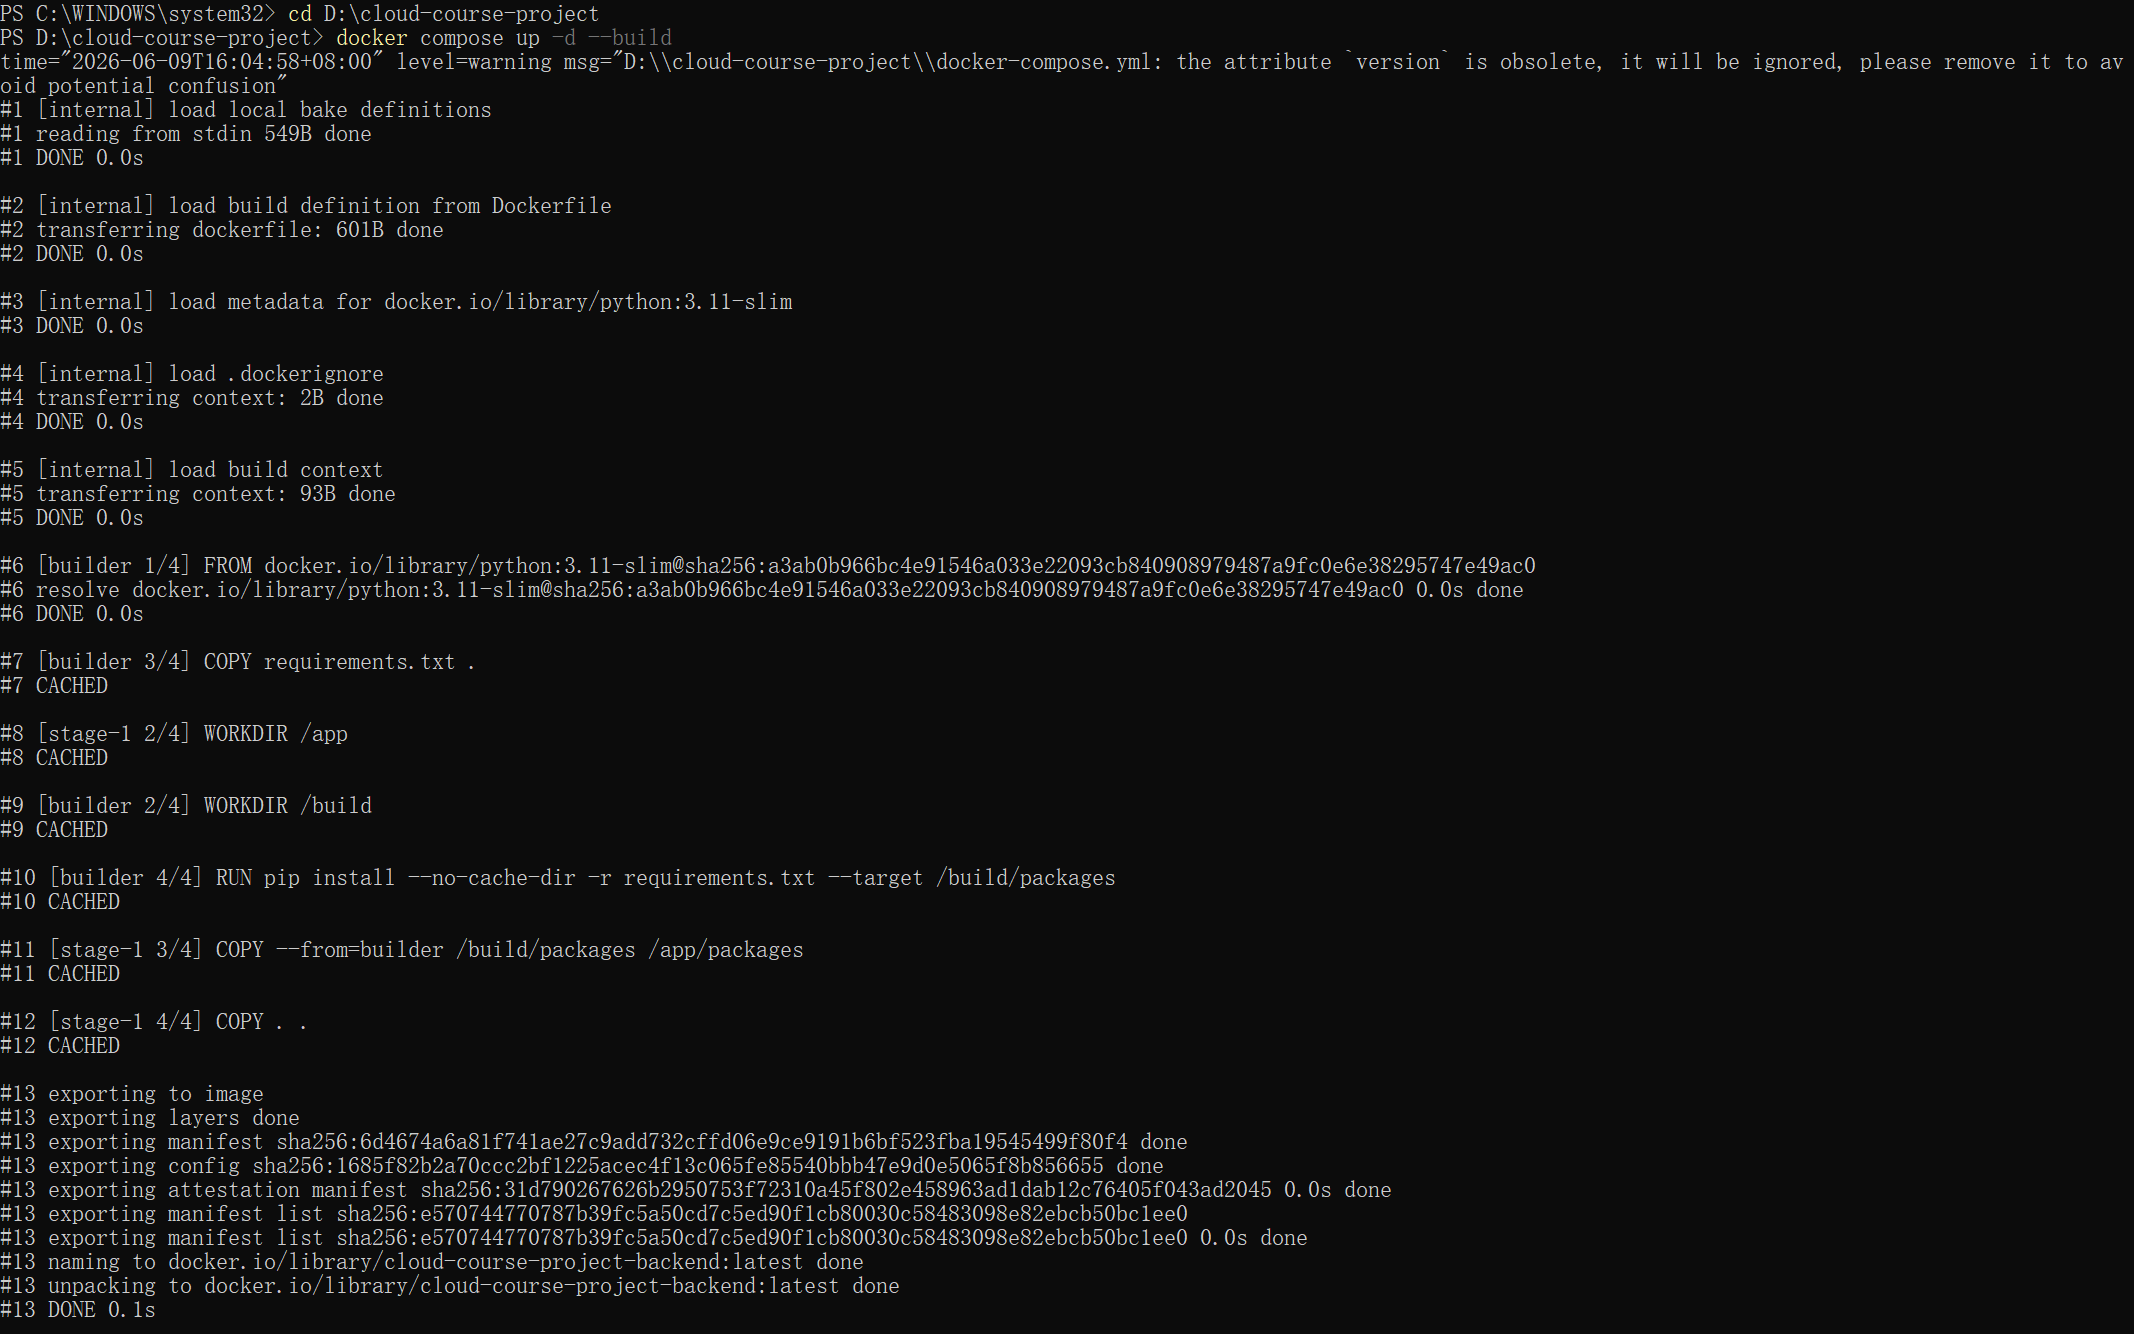
\includegraphics[width=0.92\textwidth]{assets/report_figures/overview-compose.png}
  \caption{Docker Compose 本地联调启动成功截图}
  \label{fig:overview-compose}
\end{figure}

\begin{figure}[H]
  \centering
  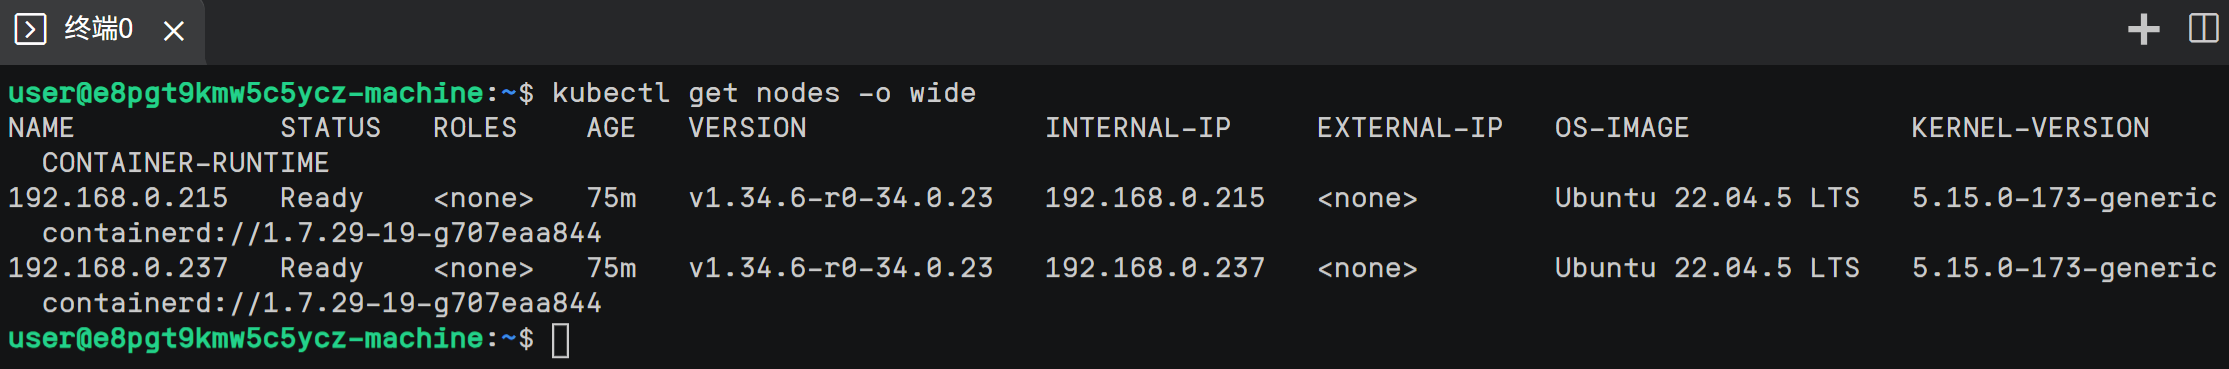
\includegraphics[width=0.92\textwidth]{assets/report_figures/overview-nodes-ready.png}
  \caption{CCE 集群两个 Worker 节点 Ready 验证截图}
  \label{fig:overview-nodes-ready}
\end{figure}

\begin{figure}[H]
  \centering
  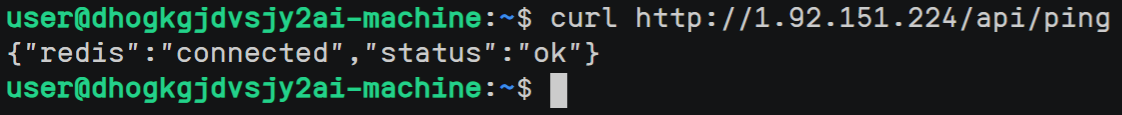
\includegraphics[width=0.92\textwidth]{assets/report_figures/overview-api-ping.png}
  \caption{通过 ELB 公网入口访问后端接口的验证截图}
  \label{fig:overview-api-ping}
\end{figure}

\subsubsection{代码仓库与报告材料说明}

本项目的代码与实验材料统一保存在课程设计仓库中。仓库根目录包含 `backend`、`frontend`、`k8s`、`spark`、`figures`、`figures\_A` 等目录，分别用于保存后端应用、前端静态页面、Kubernetes 资源文件、Spark 分析脚本和实验截图。后端部分以 Flask 提供 `/api/ping` 接口，并通过 Redis 验证服务间通信；前端部分基于 Nginx 提供静态页面和反向代理配置；`k8s` 目录保存 Deployment、Service、ConfigMap、Secret、PVC、HPA 等 YAML 文件；`spark` 目录保存 WordCount 示例、SparkApplication 模板和豆瓣电影数据分析脚本。

报告截图主要来自 `figures` 和 `figures\_A` 目录。`figures/T1` 保存应用容器化、本地联调和 SWR 镜像推送相关截图；`figures\_A/T2` 至 `figures\_A/T5` 保存 CCE 集群、应用部署、Redis 持久化和 ConfigMap Volume 挂载相关截图。后续章节将根据任务书验收要求插入截图，并在正文中说明截图反映的关键信息，例如 Pod 状态、Service 类型、ELB 公网 IP、PVC Bound 状态、Redis 数据持久化结果以及接口返回值等。通过这种组织方式，报告正文、代码文件和截图证据之间形成一一对应关系，便于检查和答辩说明。


\section{华为云实验环境}

课程设计实验主要用到华为云的 SWR、CCE、OBS 和 ELB。SWR 保存后端和前端镜像，CCE 提供 Kubernetes 集群，OBS 作为 Spark 数据读取的一种来源，ELB 用来给后端服务提供公网入口。后续部署能否跑通，基本都取决于这些资源是否先配置正确，例如 Kubernetes 版本、Worker 节点数量、节点 Ready 状态和公网访问入口。

实验区域选择华北-北京四，创建的 CCE Standard 集群名称为 \texttt{cloud-course-cce}。集群同时配置了 VPC、子网、两个 Worker 节点和负载均衡资源。为了控制代金券消耗，Worker 节点采用 2 vCPU / 4 GiB 规格；Kubernetes 版本和节点数量仍满足任务书要求。集群创建完成后，我们在 CloudShell 中检查了节点列表、集群连接信息和 kubectl 客户端版本，确认后再继续部署应用。

\subsection{云服务与资源配置}

表 \ref{tab:cloud-env-summary} 列出了本次实验实际用到的几类云服务。

\begin{table}[H]
  \centering
  \caption{华为云实验环境资源概览}
  \label{tab:cloud-env-summary}
  \small
  \renewcommand{\arraystretch}{1.22}
  \begin{tabularx}{\textwidth}{>{\raggedright\arraybackslash}p{2.0cm} >{\raggedright\arraybackslash}p{2.6cm} Y}
    \toprule
    云服务 & 本项目用途 & 关键配置或说明 \\
    \midrule
    SWR & 容器镜像仓库 & 保存 \texttt{backend:v1} 与 \texttt{frontend:v1} 镜像，为 CCE Deployment 提供镜像来源。 \\
    CCE & Kubernetes 集群 & 创建 \texttt{cloud-course-cce} 集群，版本为 v1.34，包含 2 个 Worker 节点。 \\
    OBS & Spark 数据存储接口 & Spark 脚本支持通过 \texttt{s3a://} 路径读取数据；当前报告中 Spark 章节将结合数据分析脚本展开说明。 \\
    ELB & 公网负载均衡 & 后端 \texttt{backend-svc} 通过共享型公网 ELB 暴露 \texttt{/api/ping} 接口。 \\
    \bottomrule
  \end{tabularx}
\end{table}

\subsubsection{SWR镜像仓库配置}

SWR 是本项目中连接本地容器构建与云端 Kubernetes 部署的关键环节。后端 Flask 服务和前端 Nginx 服务在本地完成 Docker 镜像构建后，需要推送至华为云 SWR，随后 CCE 节点才能在创建 Pod 时从私有镜像仓库拉取镜像。由于 SWR 镜像仓库通常为私有仓库，后续 Deployment 中还需要结合镜像拉取密钥或 CCE 自动生成的 \texttt{default-secret} 进行鉴权。

\begin{figure}[H]
  \centering
  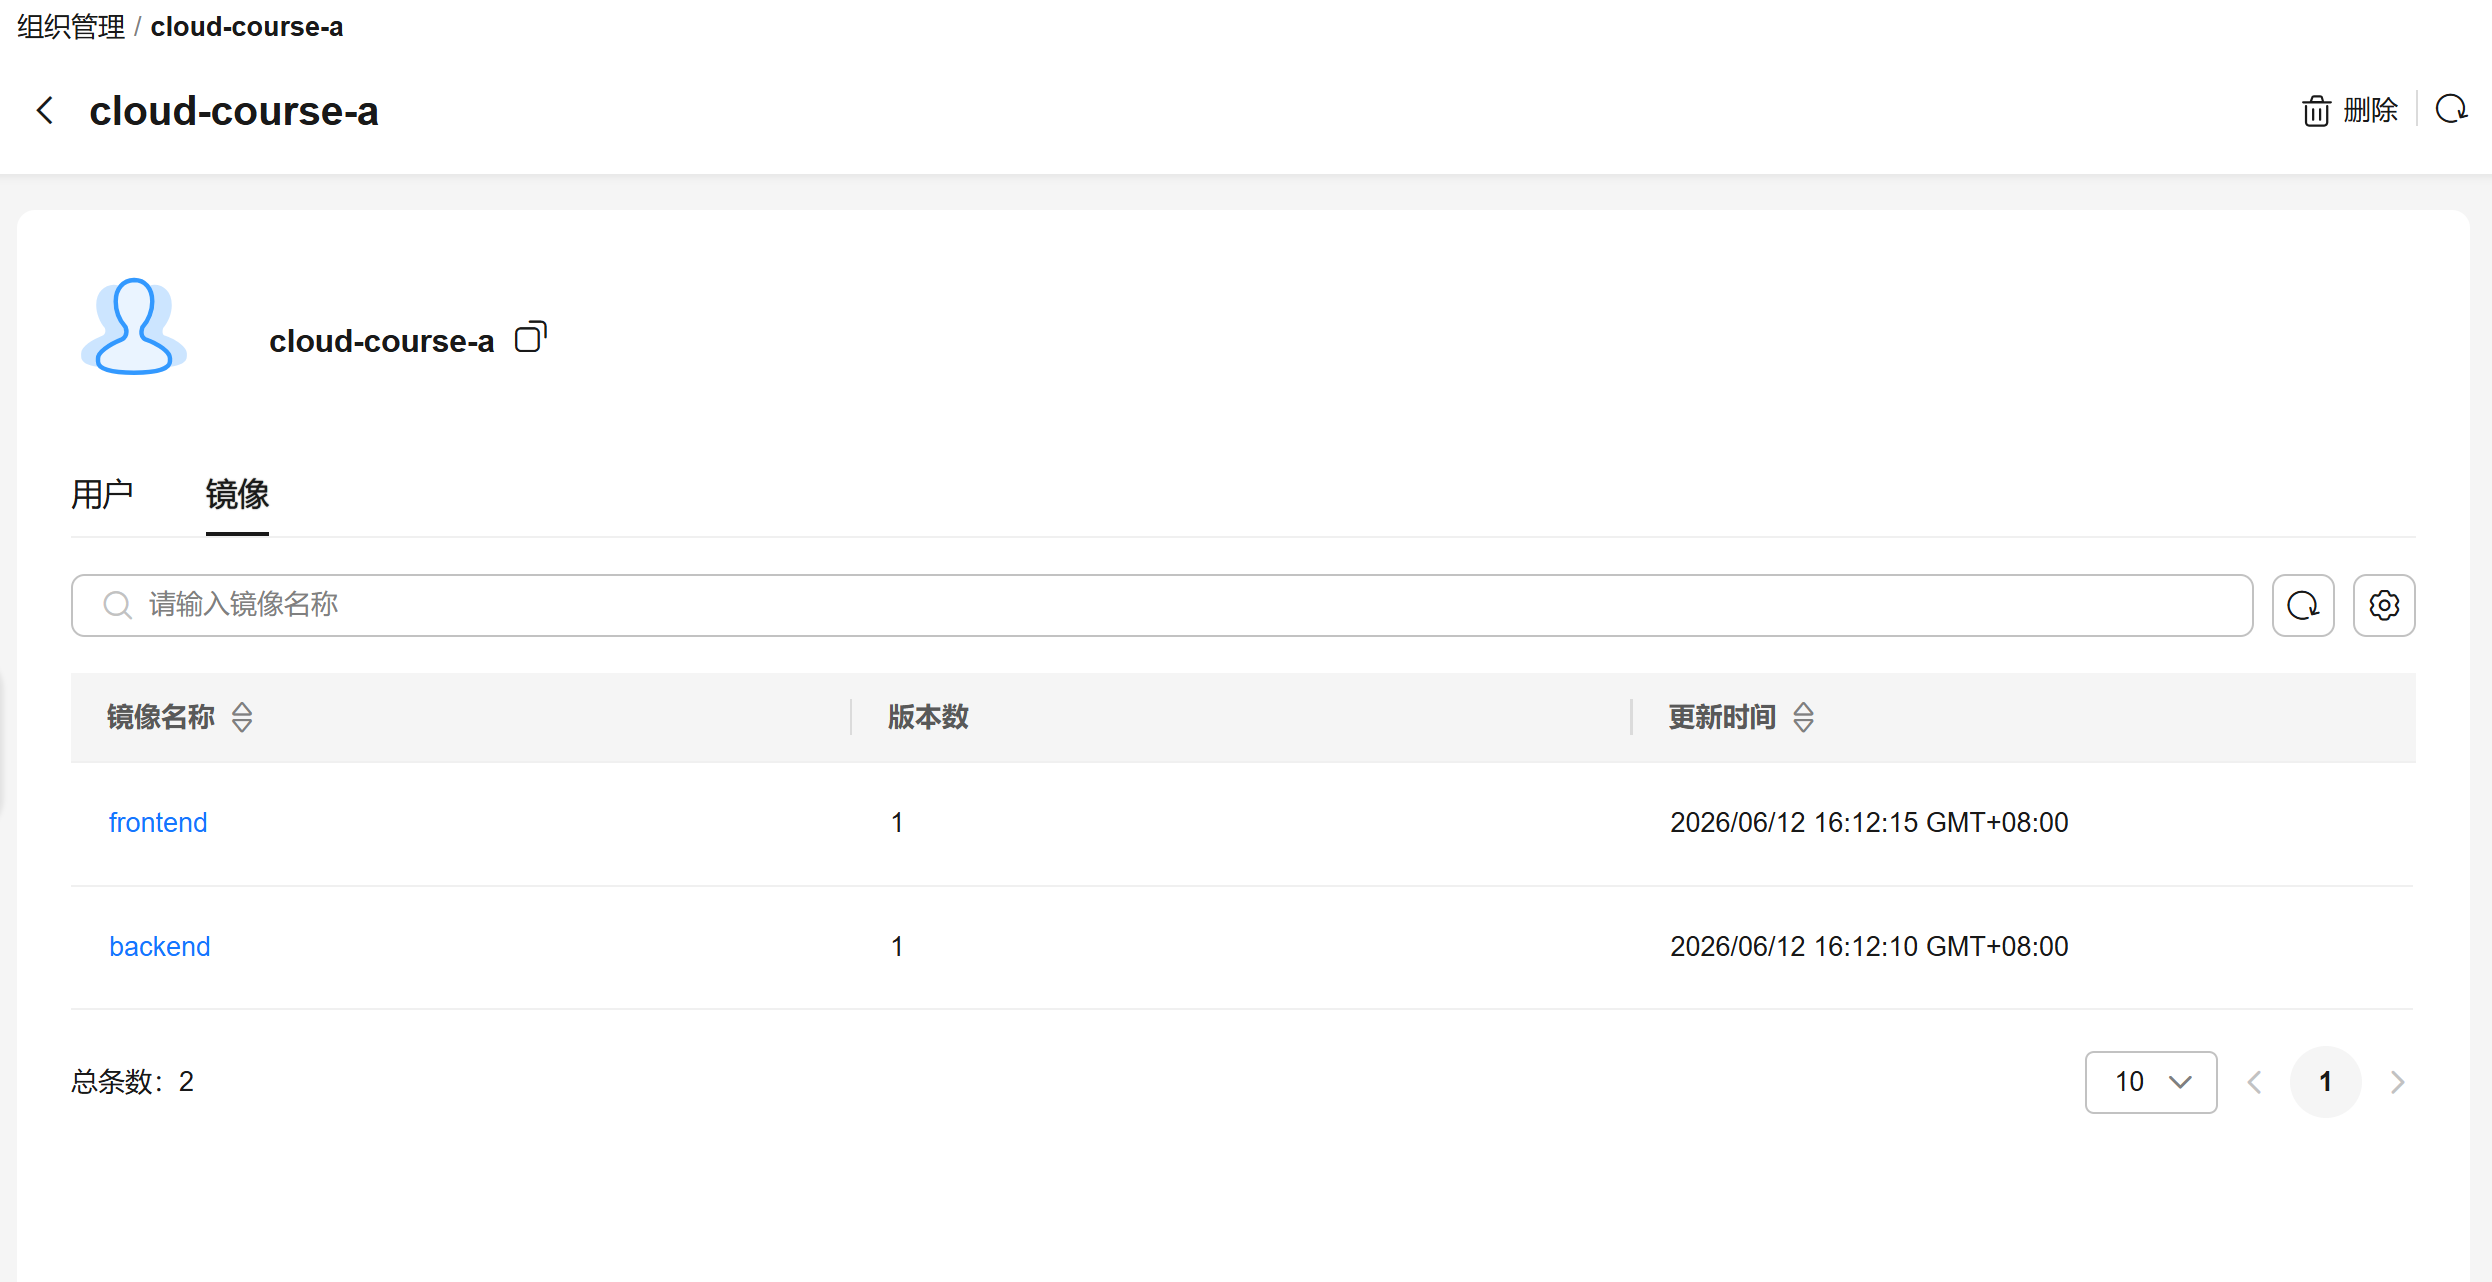
\includegraphics[width=0.92\textwidth]{assets/report_figures/env/env-swr-images.png}
  \caption{SWR 中 backend 与 frontend 镜像确认截图}
  \label{fig:env-swr-images}
\end{figure}

图 \ref{fig:env-swr-images} 中可以看到，郑瑞璟的 SWR 组织下已经有 \texttt{backend} 和 \texttt{frontend} 两个镜像，标签均为 \texttt{v1}。后续 CCE 部署引用的就是这里的镜像地址；如果私有镜像拉取失败，则需要在 Deployment 中配合 \texttt{imagePullSecrets} 处理鉴权问题。

\subsubsection{CCE集群配置}

CCE 是第一部分云计算平台搭建的核心服务。项目创建的是 CCE Standard 集群，集群名称为 \texttt{cloud-course-cce}，区域为华北-北京四，Kubernetes 版本为 v1.34，满足任务书中“集群版本不低于 1.27”的要求。网络方面，集群绑定 VPC \texttt{cloud-course-vpc}，网段为 \texttt{192.168.0.0/16}；子网名称为 \texttt{cloud-course-subnet}，网段为 \texttt{192.168.0.0/24}。节点方面，集群创建 2 个 Worker 节点，节点规格为 \texttt{c9.large.2}，即 2 vCPU / 4 GiB，操作系统为 Ubuntu 22.04.5 LTS，容器运行时为 containerd。

\begin{figure}[H]
  \centering
  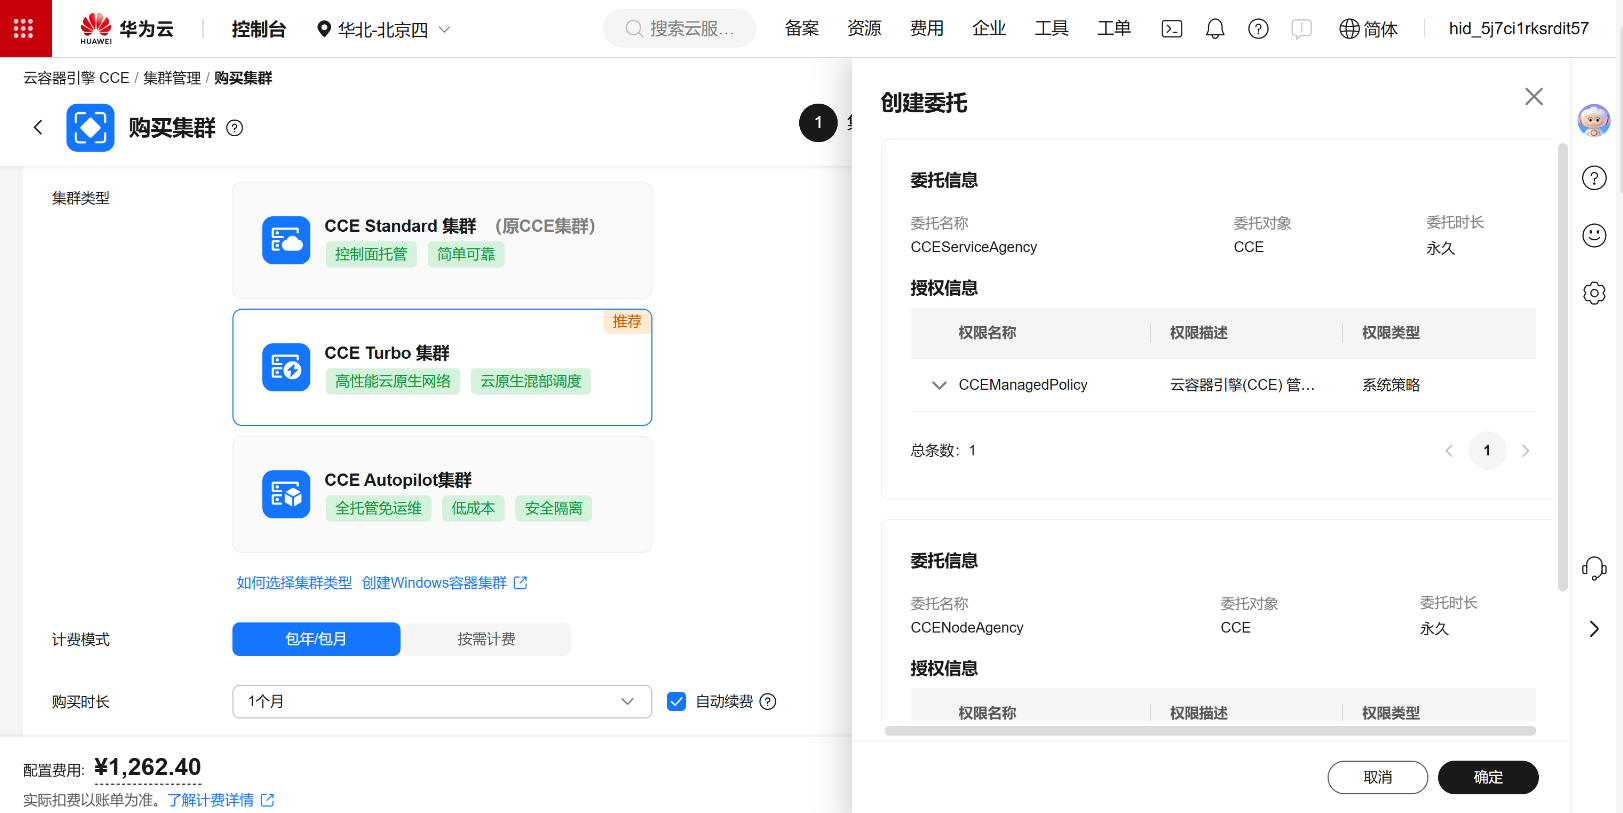
\includegraphics[width=0.92\textwidth]{assets/report_figures/t2/t2-01-cce-agency.png}
  \caption{首次使用 CCE 时创建服务委托截图}
  \label{fig:t2-cce-agency}
\end{figure}

图 \ref{fig:t2-cce-agency} 显示了首次使用 CCE 时创建服务委托的过程。CCE 作为托管 Kubernetes 服务，需要通过服务委托访问部分云资源，例如负载均衡、存储和网络资源。该步骤是后续自动创建或绑定云端资源的前置条件。

\begin{figure}[H]
  \centering
  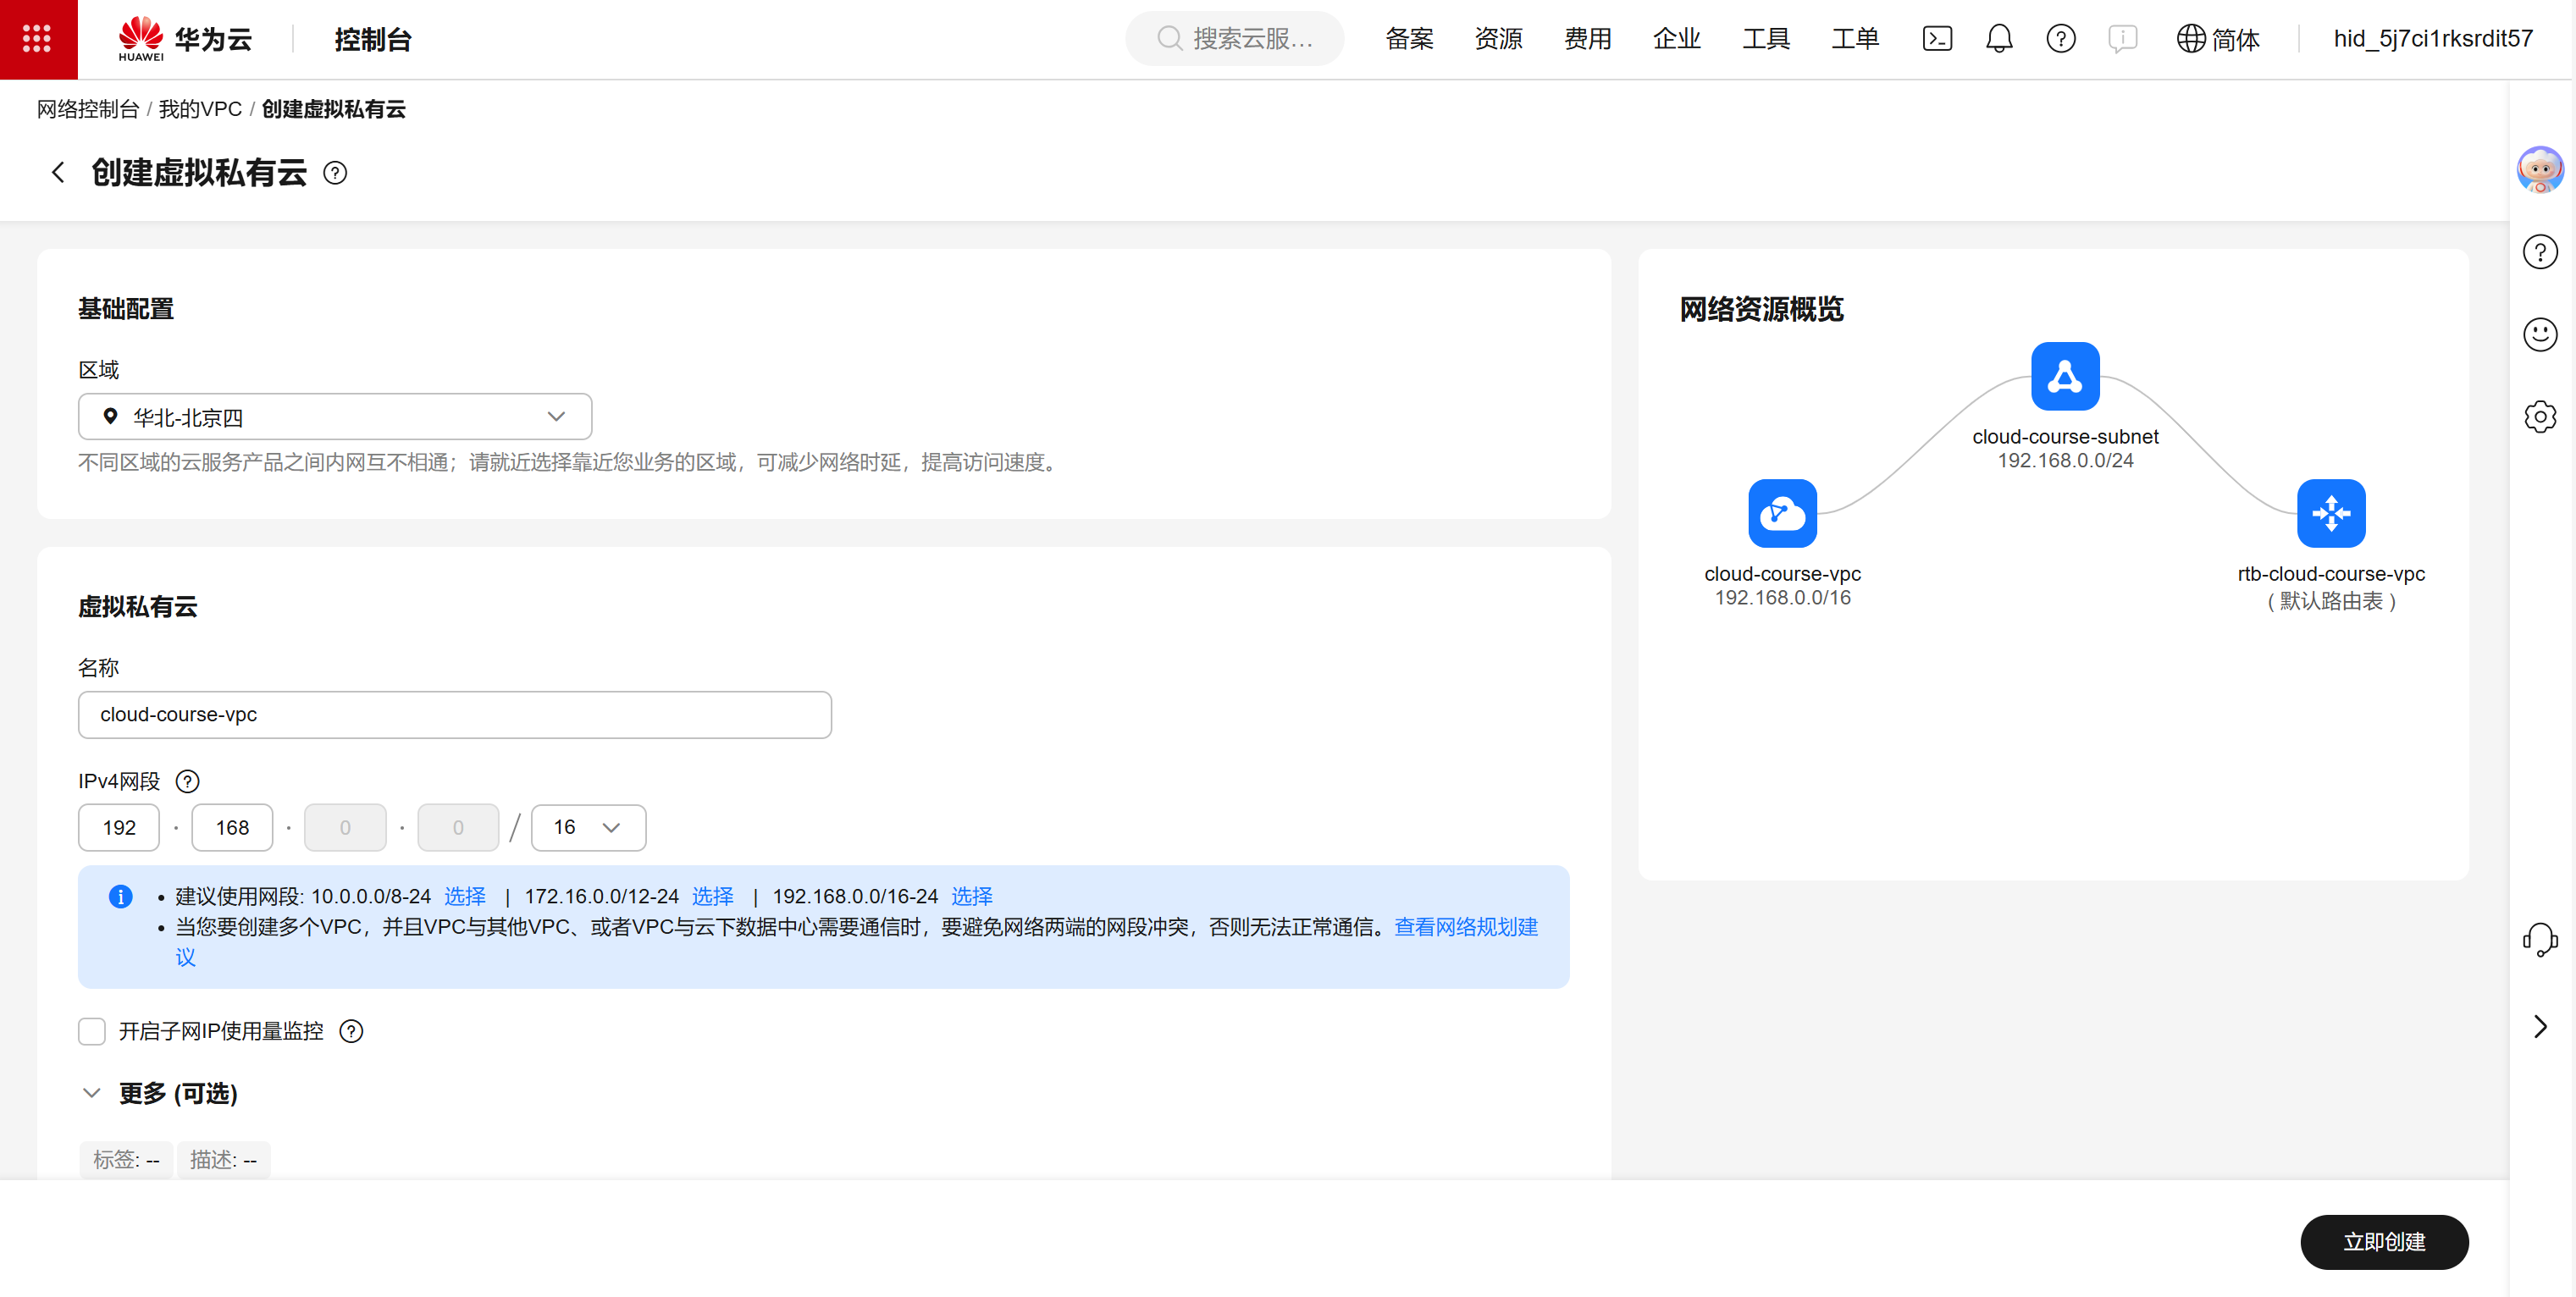
\includegraphics[width=0.92\textwidth]{assets/report_figures/t2/t2-02-vpc-subnet-config.png}
  \caption{创建 VPC 与子网配置页面截图}
  \label{fig:t2-vpc-subnet-config}
\end{figure}

图 \ref{fig:t2-vpc-subnet-config} 展示了 VPC 和子网的创建配置。VPC 为 CCE 节点、Pod 网络和云端负载均衡提供基础网络隔离环境，子网则决定 Worker 节点实际使用的内网地址范围。本项目使用统一命名的 \texttt{cloud-course-vpc} 和 \texttt{cloud-course-subnet}，便于后续资源定位和排错。

\begin{figure}[H]
  \centering
  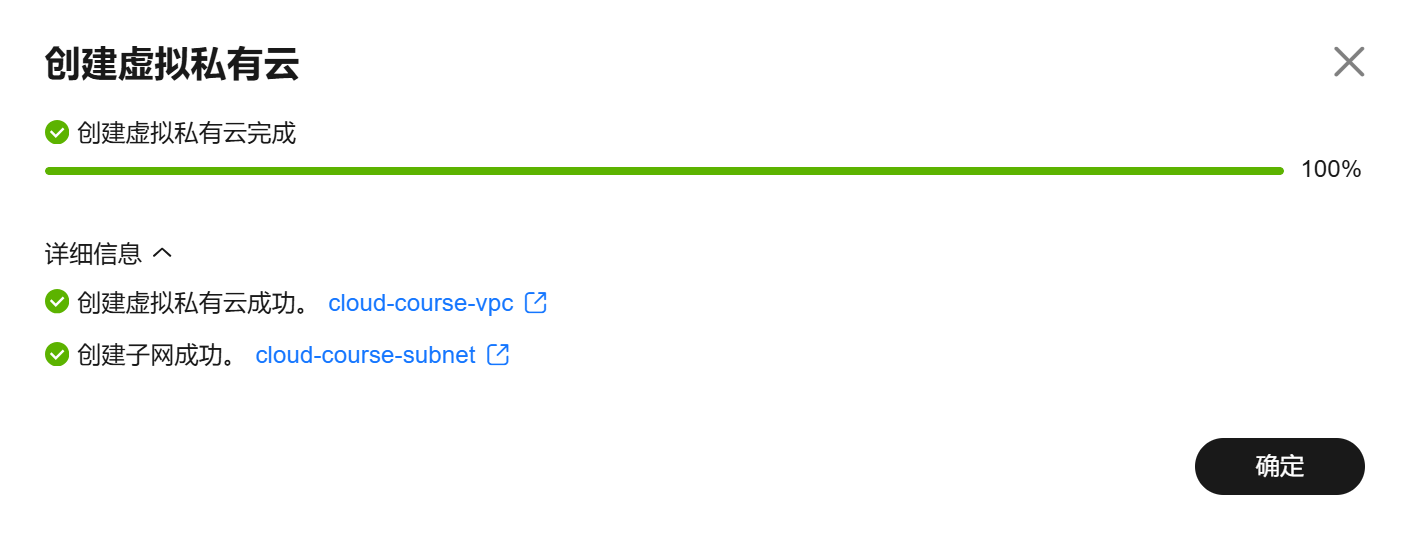
\includegraphics[width=0.92\textwidth]{assets/report_figures/t2/t2-03-vpc-subnet-created.png}
  \caption{VPC 与子网创建成功截图}
  \label{fig:t2-vpc-subnet-created}
\end{figure}

图 \ref{fig:t2-vpc-subnet-created} 表明 VPC 和子网已经创建完成。该结果说明 CCE 集群创建前的网络基础资源已经就绪，后续 Worker 节点可以加入该网络并获得内网 IP。

\begin{figure}[H]
  \centering
  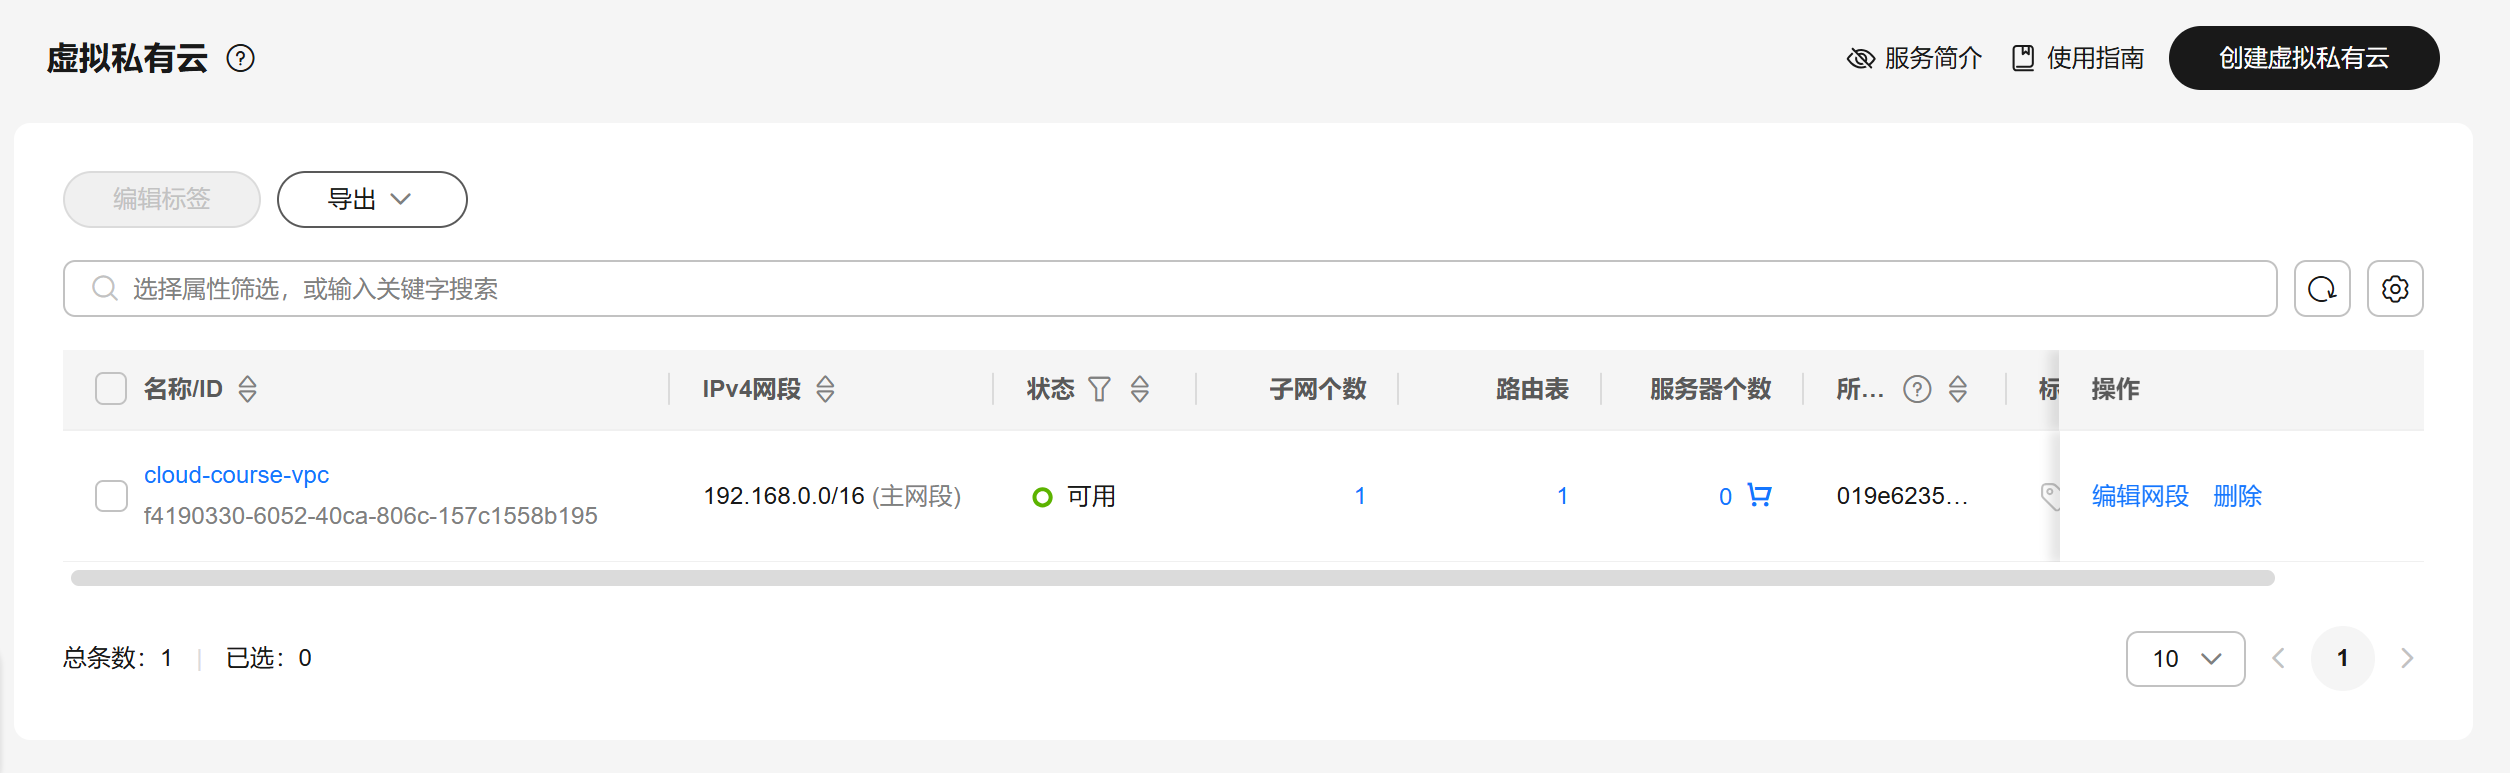
\includegraphics[width=0.92\textwidth]{assets/report_figures/t2/t2-04-vpc-list.png}
  \caption{VPC 列表中 cloud-course-vpc 状态可用截图}
  \label{fig:t2-vpc-list}
\end{figure}

图 \ref{fig:t2-vpc-list} 中，\texttt{cloud-course-vpc} 已处于可用状态。

\begin{figure}[H]
  \centering
  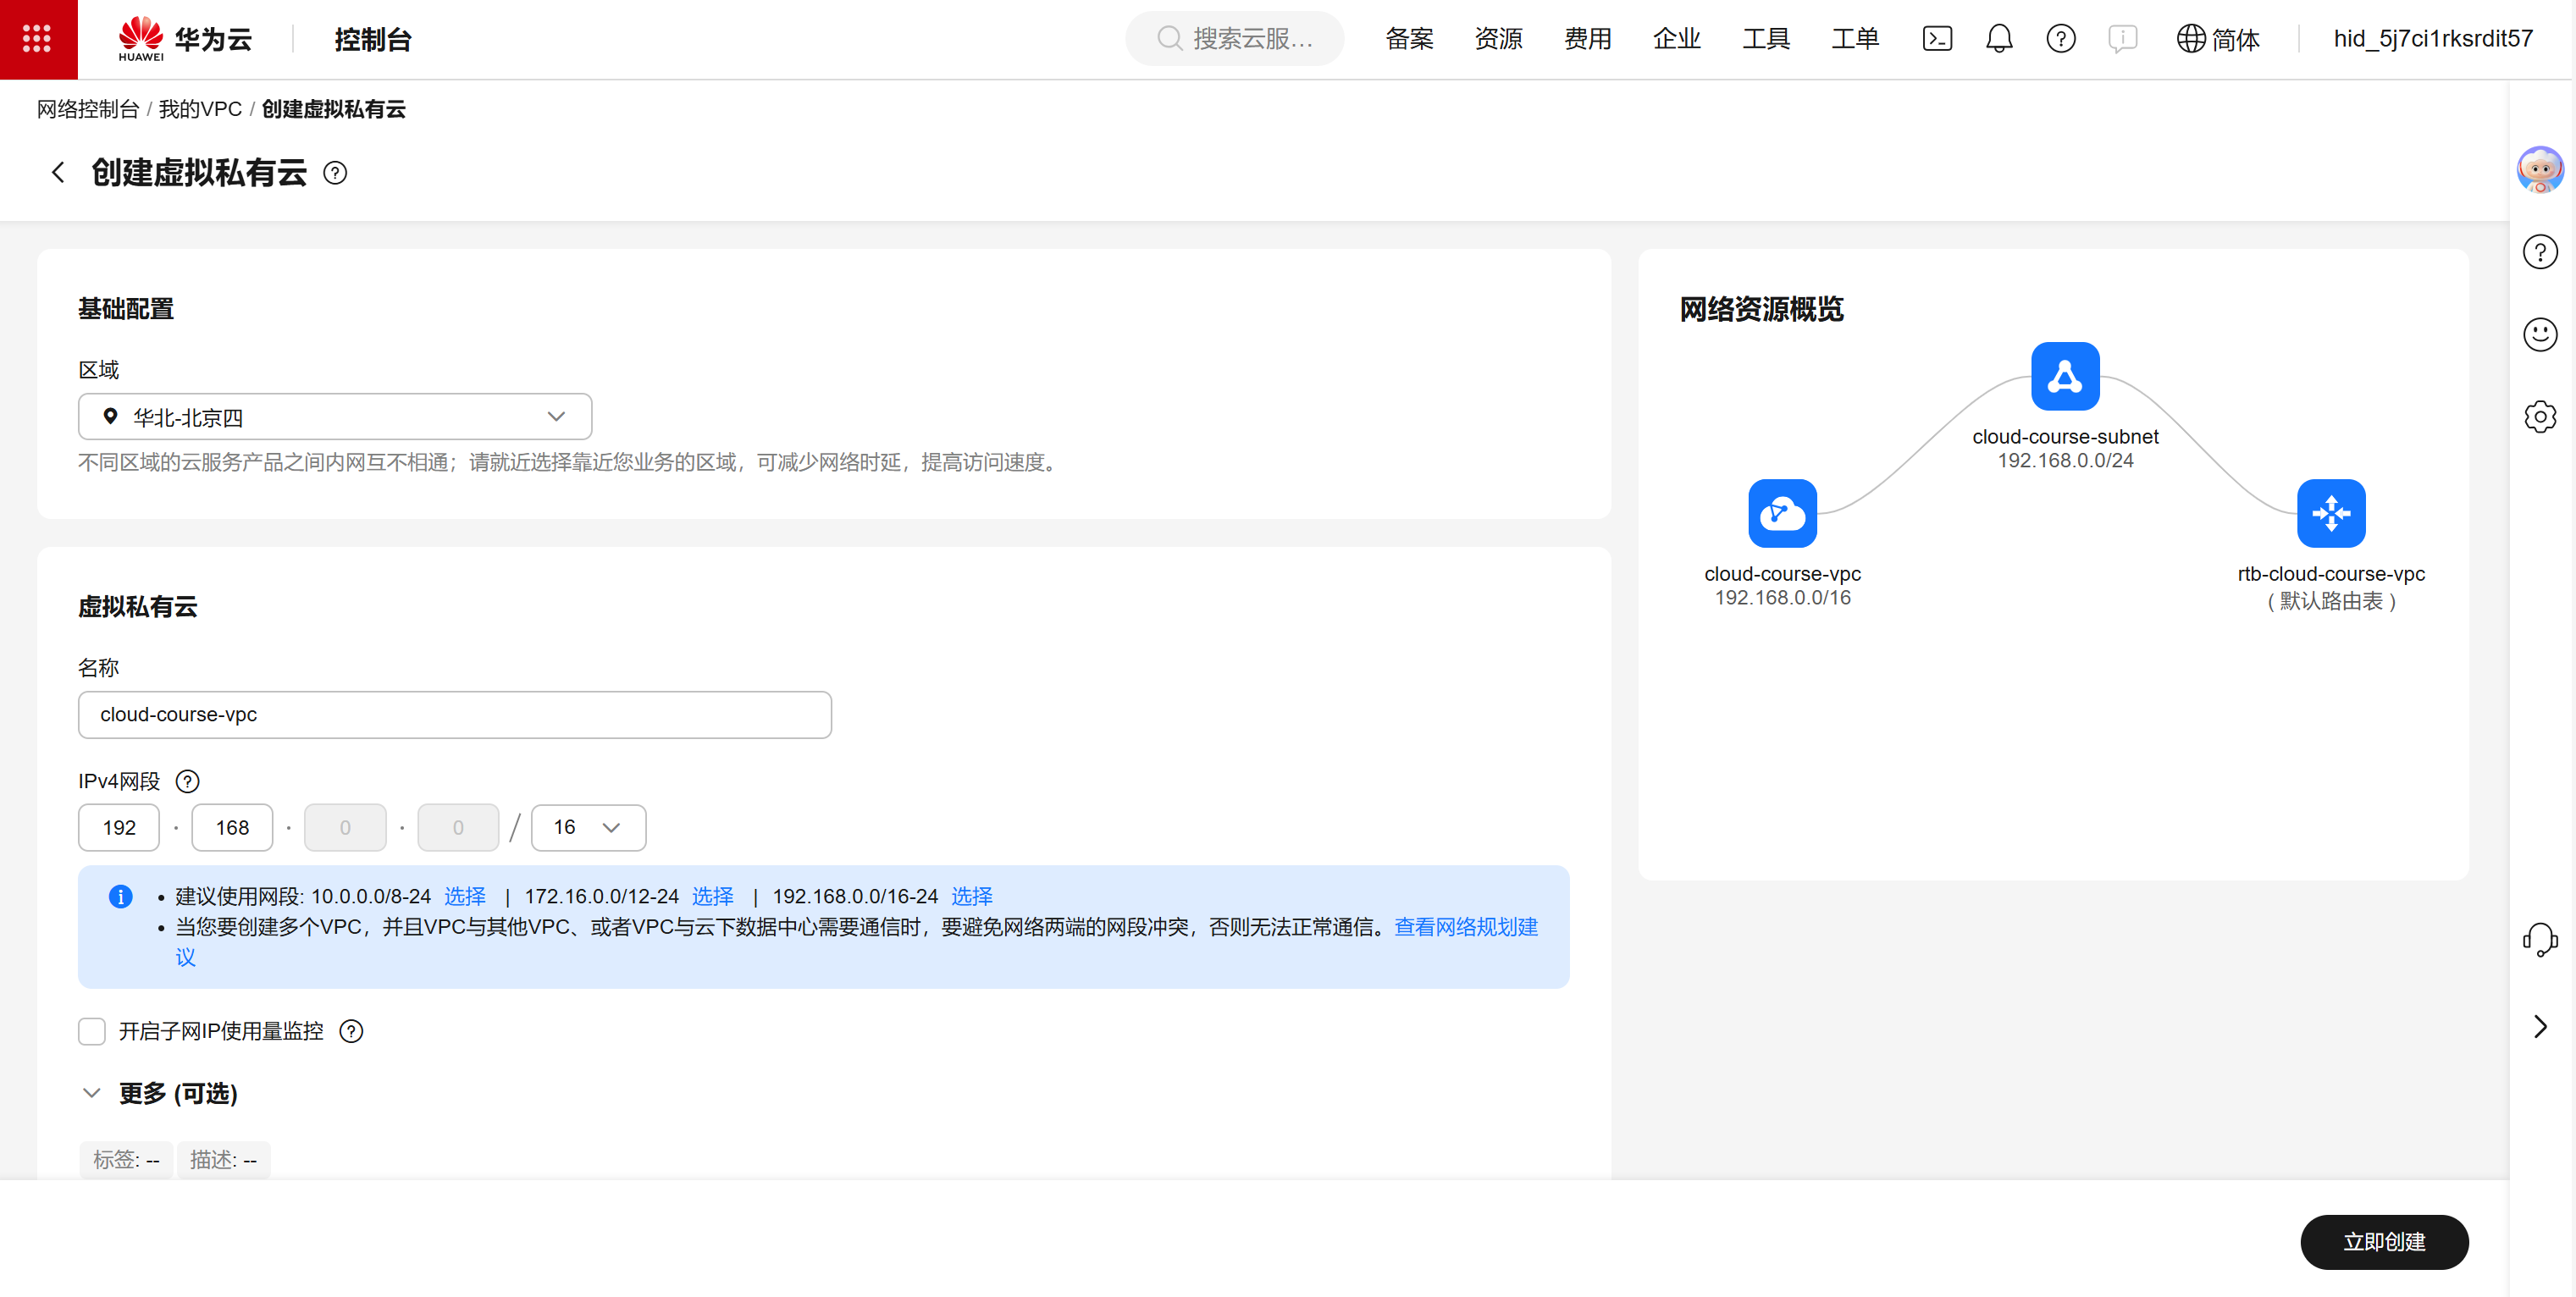
\includegraphics[width=0.92\textwidth]{assets/report_figures/t2/t2-05-cce-network-overview.png}
  \caption{CCE 集群网络配置总览截图}
  \label{fig:t2-cce-network-overview}
\end{figure}

图 \ref{fig:t2-cce-network-overview} 展示了 CCE 集群创建时的网络配置总览，页面中能看到集群绑定的 VPC、子网和容器网络配置。

\begin{figure}[H]
  \centering
  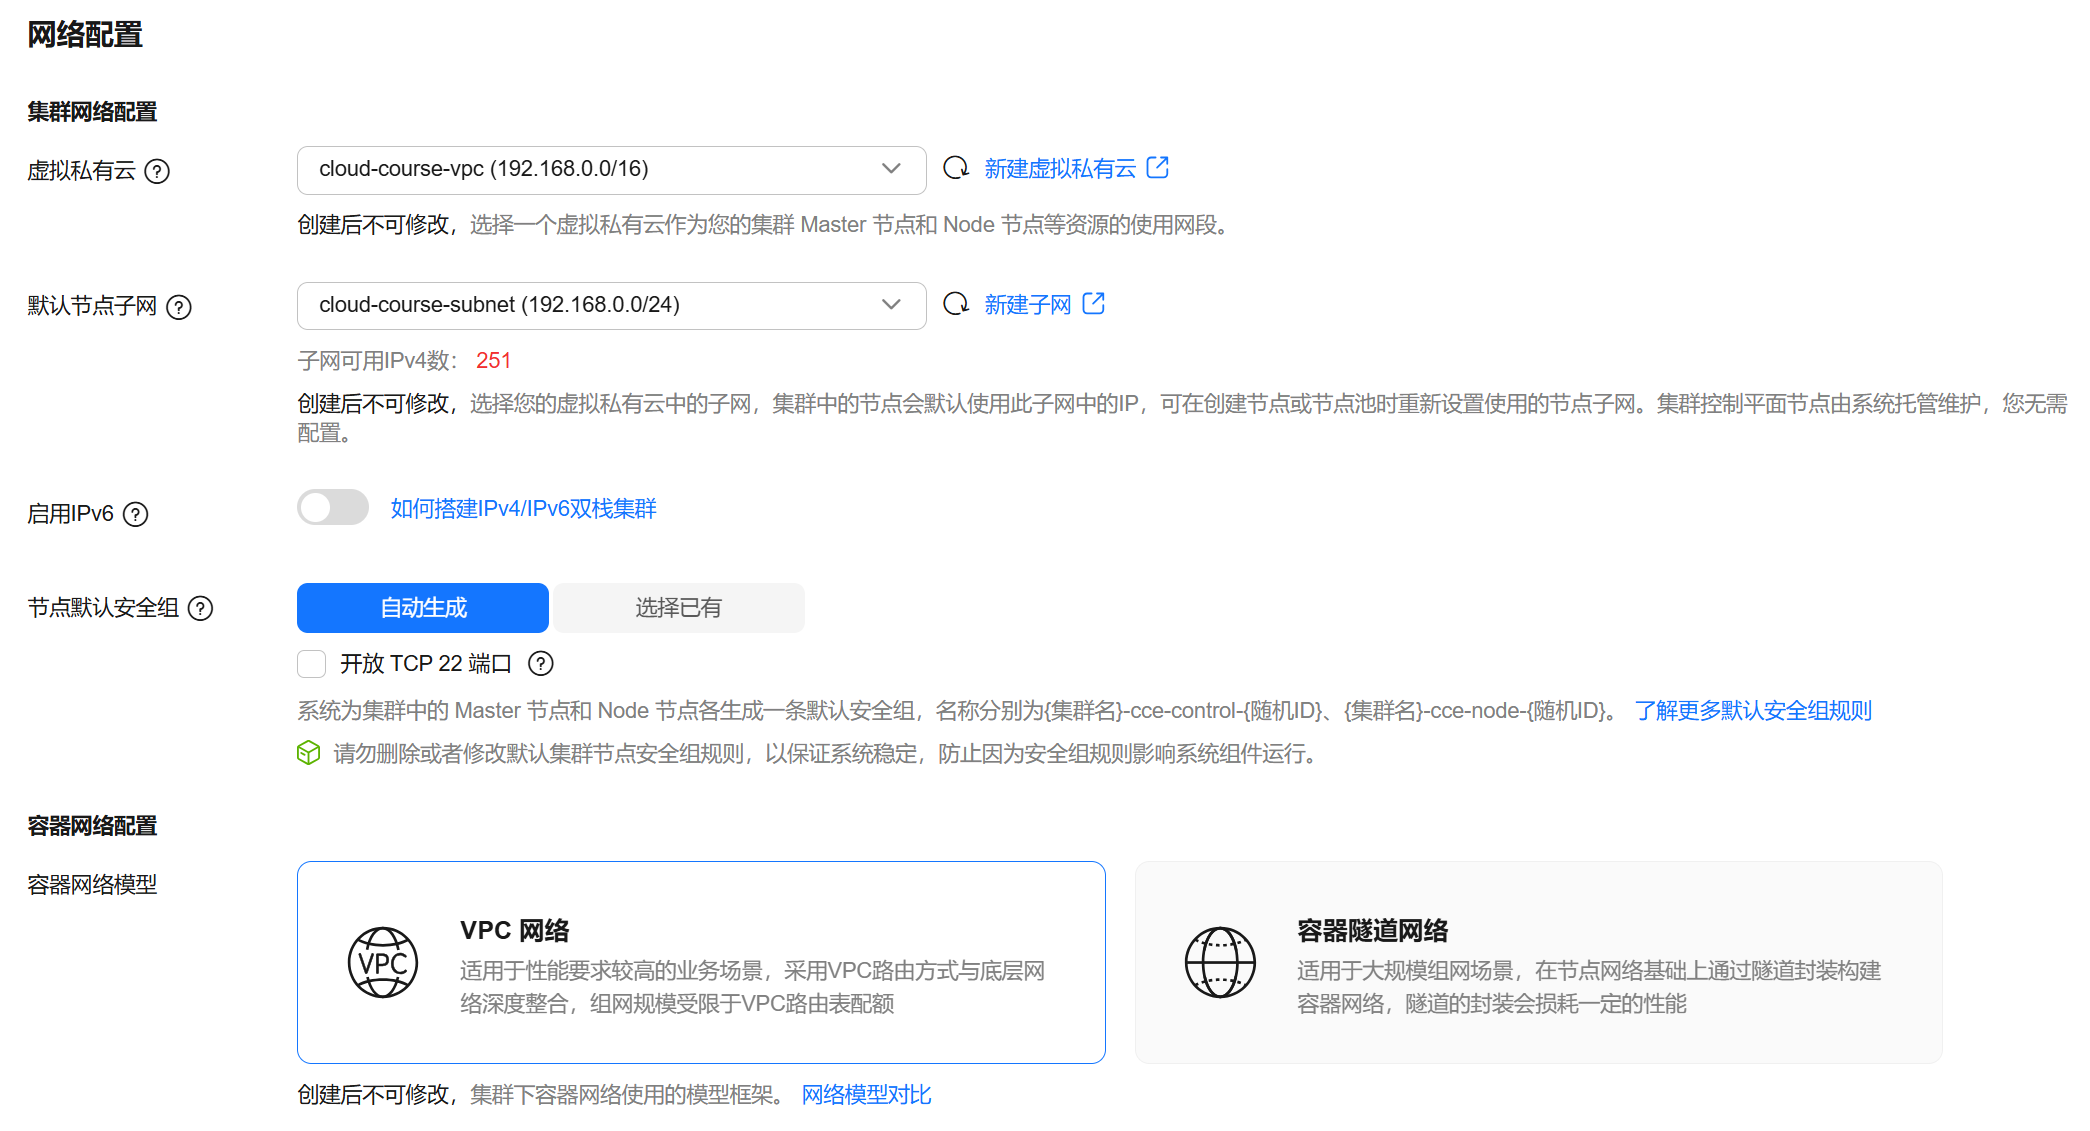
\includegraphics[width=0.92\textwidth]{assets/report_figures/t2/t2-06-cce-network-model.png}
  \caption{CCE 网络配置中 VPC、子网和容器网络模型截图}
  \label{fig:t2-cce-network-model}
\end{figure}

图 \ref{fig:t2-cce-network-model} 展示了 CCE 网络模型配置，可以看到集群使用的 VPC、子网和容器网络模型。

\begin{figure}[H]
  \centering
  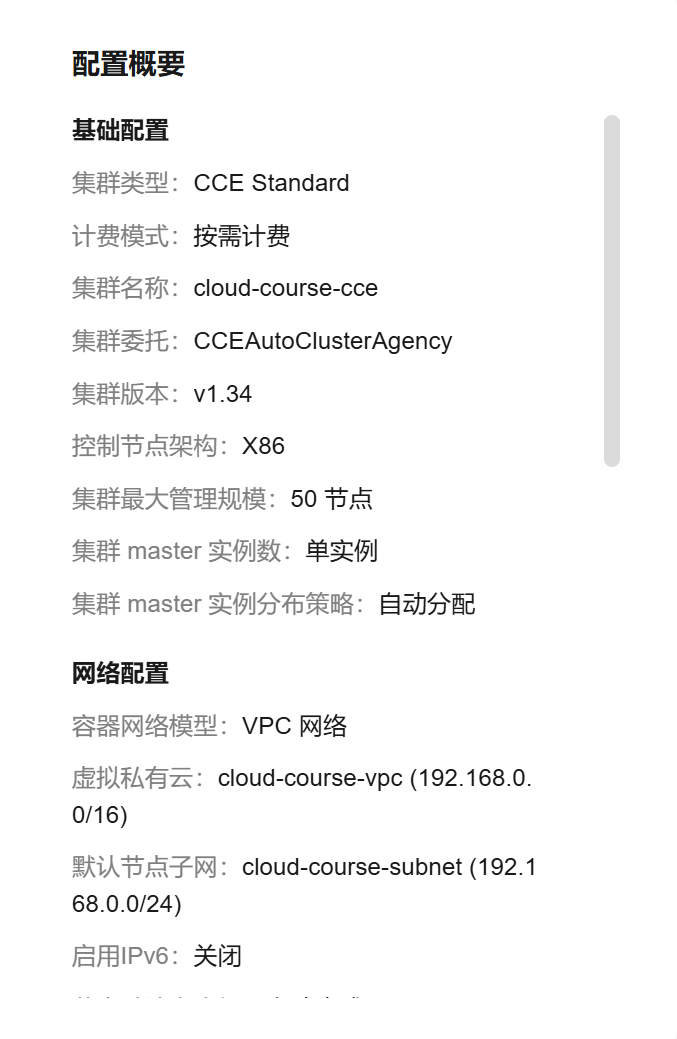
\includegraphics[width=0.68\textwidth]{assets/report_figures/t2/t2-07-cce-basic-summary.png}
  \caption{CCE 基础配置概要截图}
  \label{fig:t2-cce-basic-summary}
\end{figure}

图 \ref{fig:t2-cce-basic-summary} 中可以看到集群名称、集群类型和 Kubernetes 版本。

\begin{figure}[H]
  \centering
  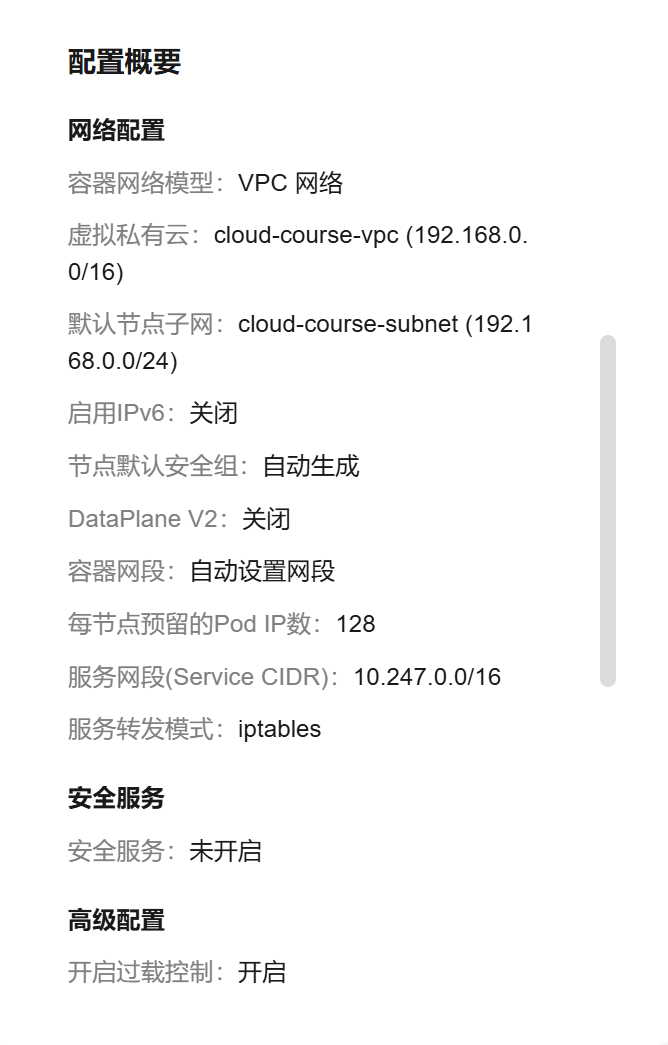
\includegraphics[width=0.55\textwidth]{assets/report_figures/t2/t2-09-cce-security-summary.png}
  \caption{CCE 网络与安全服务配置概要截图}
  \label{fig:t2-cce-security-summary}
\end{figure}

图 \ref{fig:t2-cce-security-summary} 展示了网络与安全服务配置，包括安全组和相关云服务选项。

\begin{figure}[H]
  \centering
  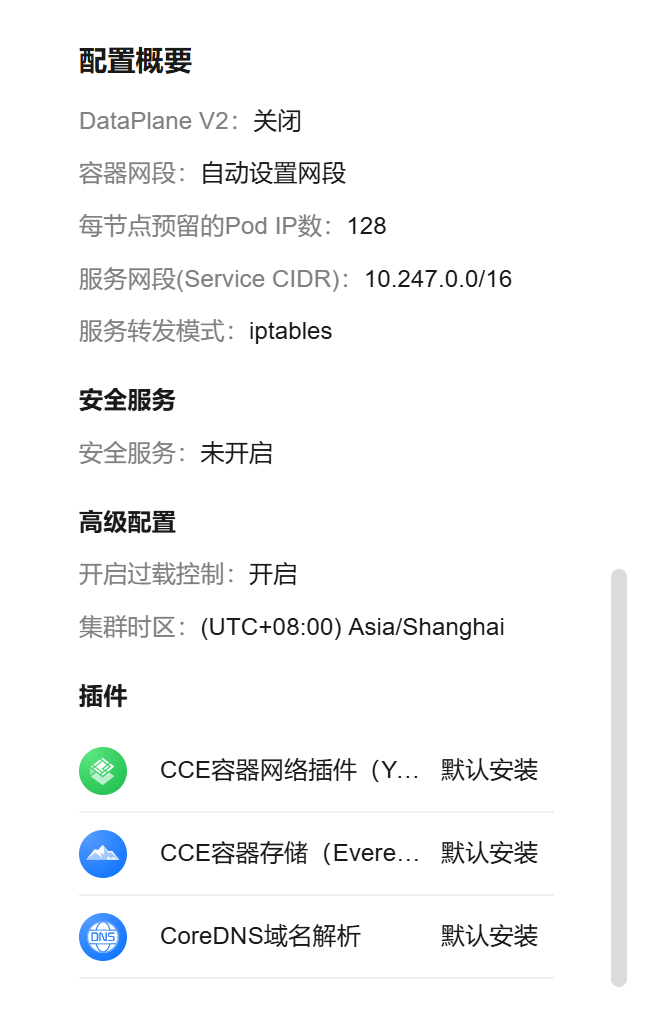
\includegraphics[width=0.55\textwidth]{assets/report_figures/t2/t2-10-cce-plugin-summary.png}
  \caption{CCE 网络与默认插件配置概要截图}
  \label{fig:t2-cce-plugin-summary}
\end{figure}

图 \ref{fig:t2-cce-plugin-summary} 展示了网络配置和默认插件配置。这里保留 CoreDNS、存储插件和容器网络插件，用于后续 Pod 通信、服务名解析和 PVC 挂载。

\begin{figure}[H]
  \centering
  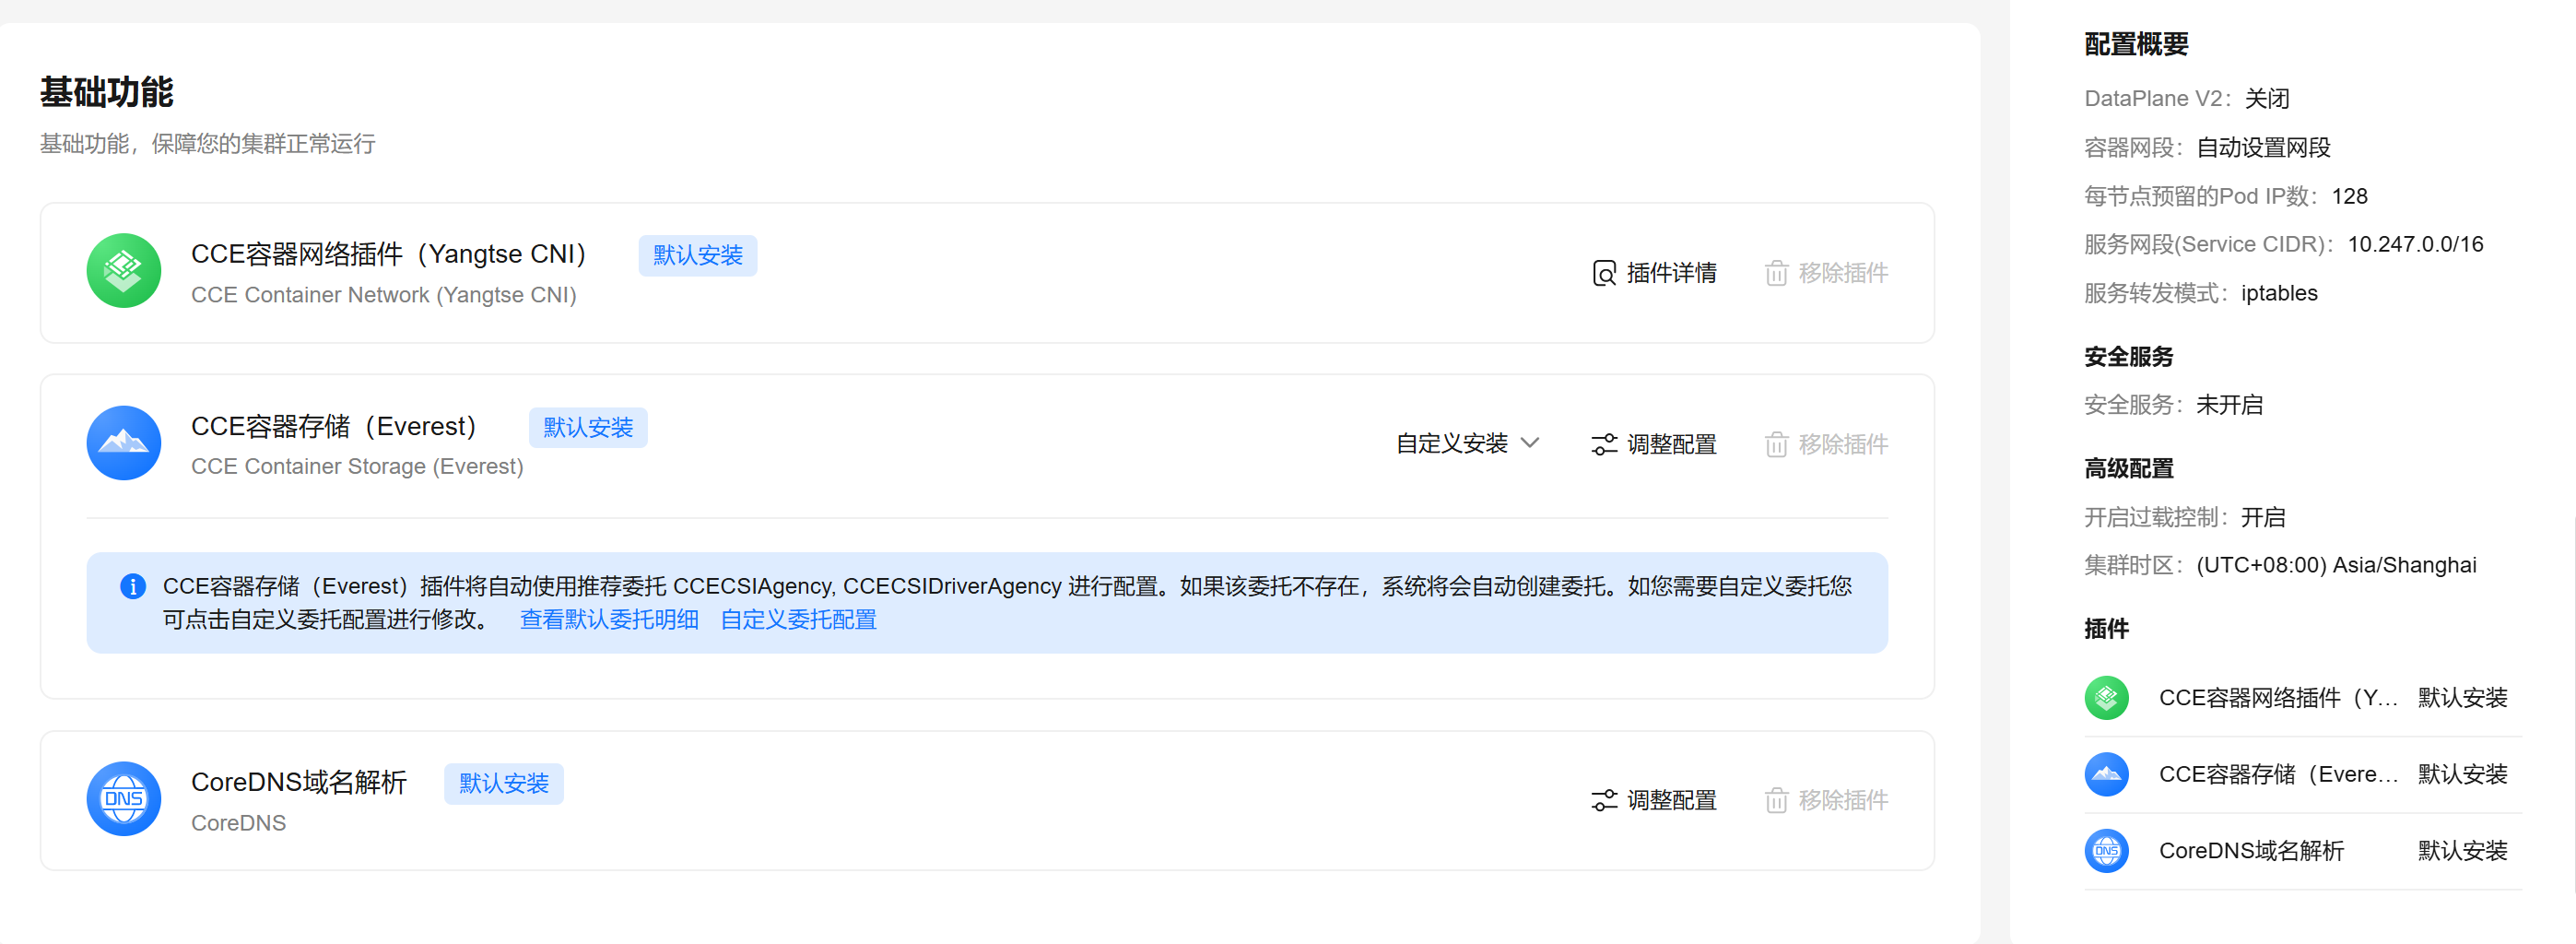
\includegraphics[width=0.92\textwidth]{assets/report_figures/t2/t2-11-cce-plugins.png}
  \caption{CCE 默认必要插件配置截图}
  \label{fig:t2-cce-plugins}
\end{figure}

图 \ref{fig:t2-cce-plugins} 展示了 CCE 集群创建时保留的默认必要插件。CoreDNS 用于集群内部服务名解析，Everest 存储插件用于后续 PVC 与云硬盘的对接，容器网络插件用于 Pod 网络通信。这些插件虽然不是业务应用代码的一部分，但它们决定了 Kubernetes 集群是否具备完整的基础能力。

\begin{figure}[H]
  \centering
  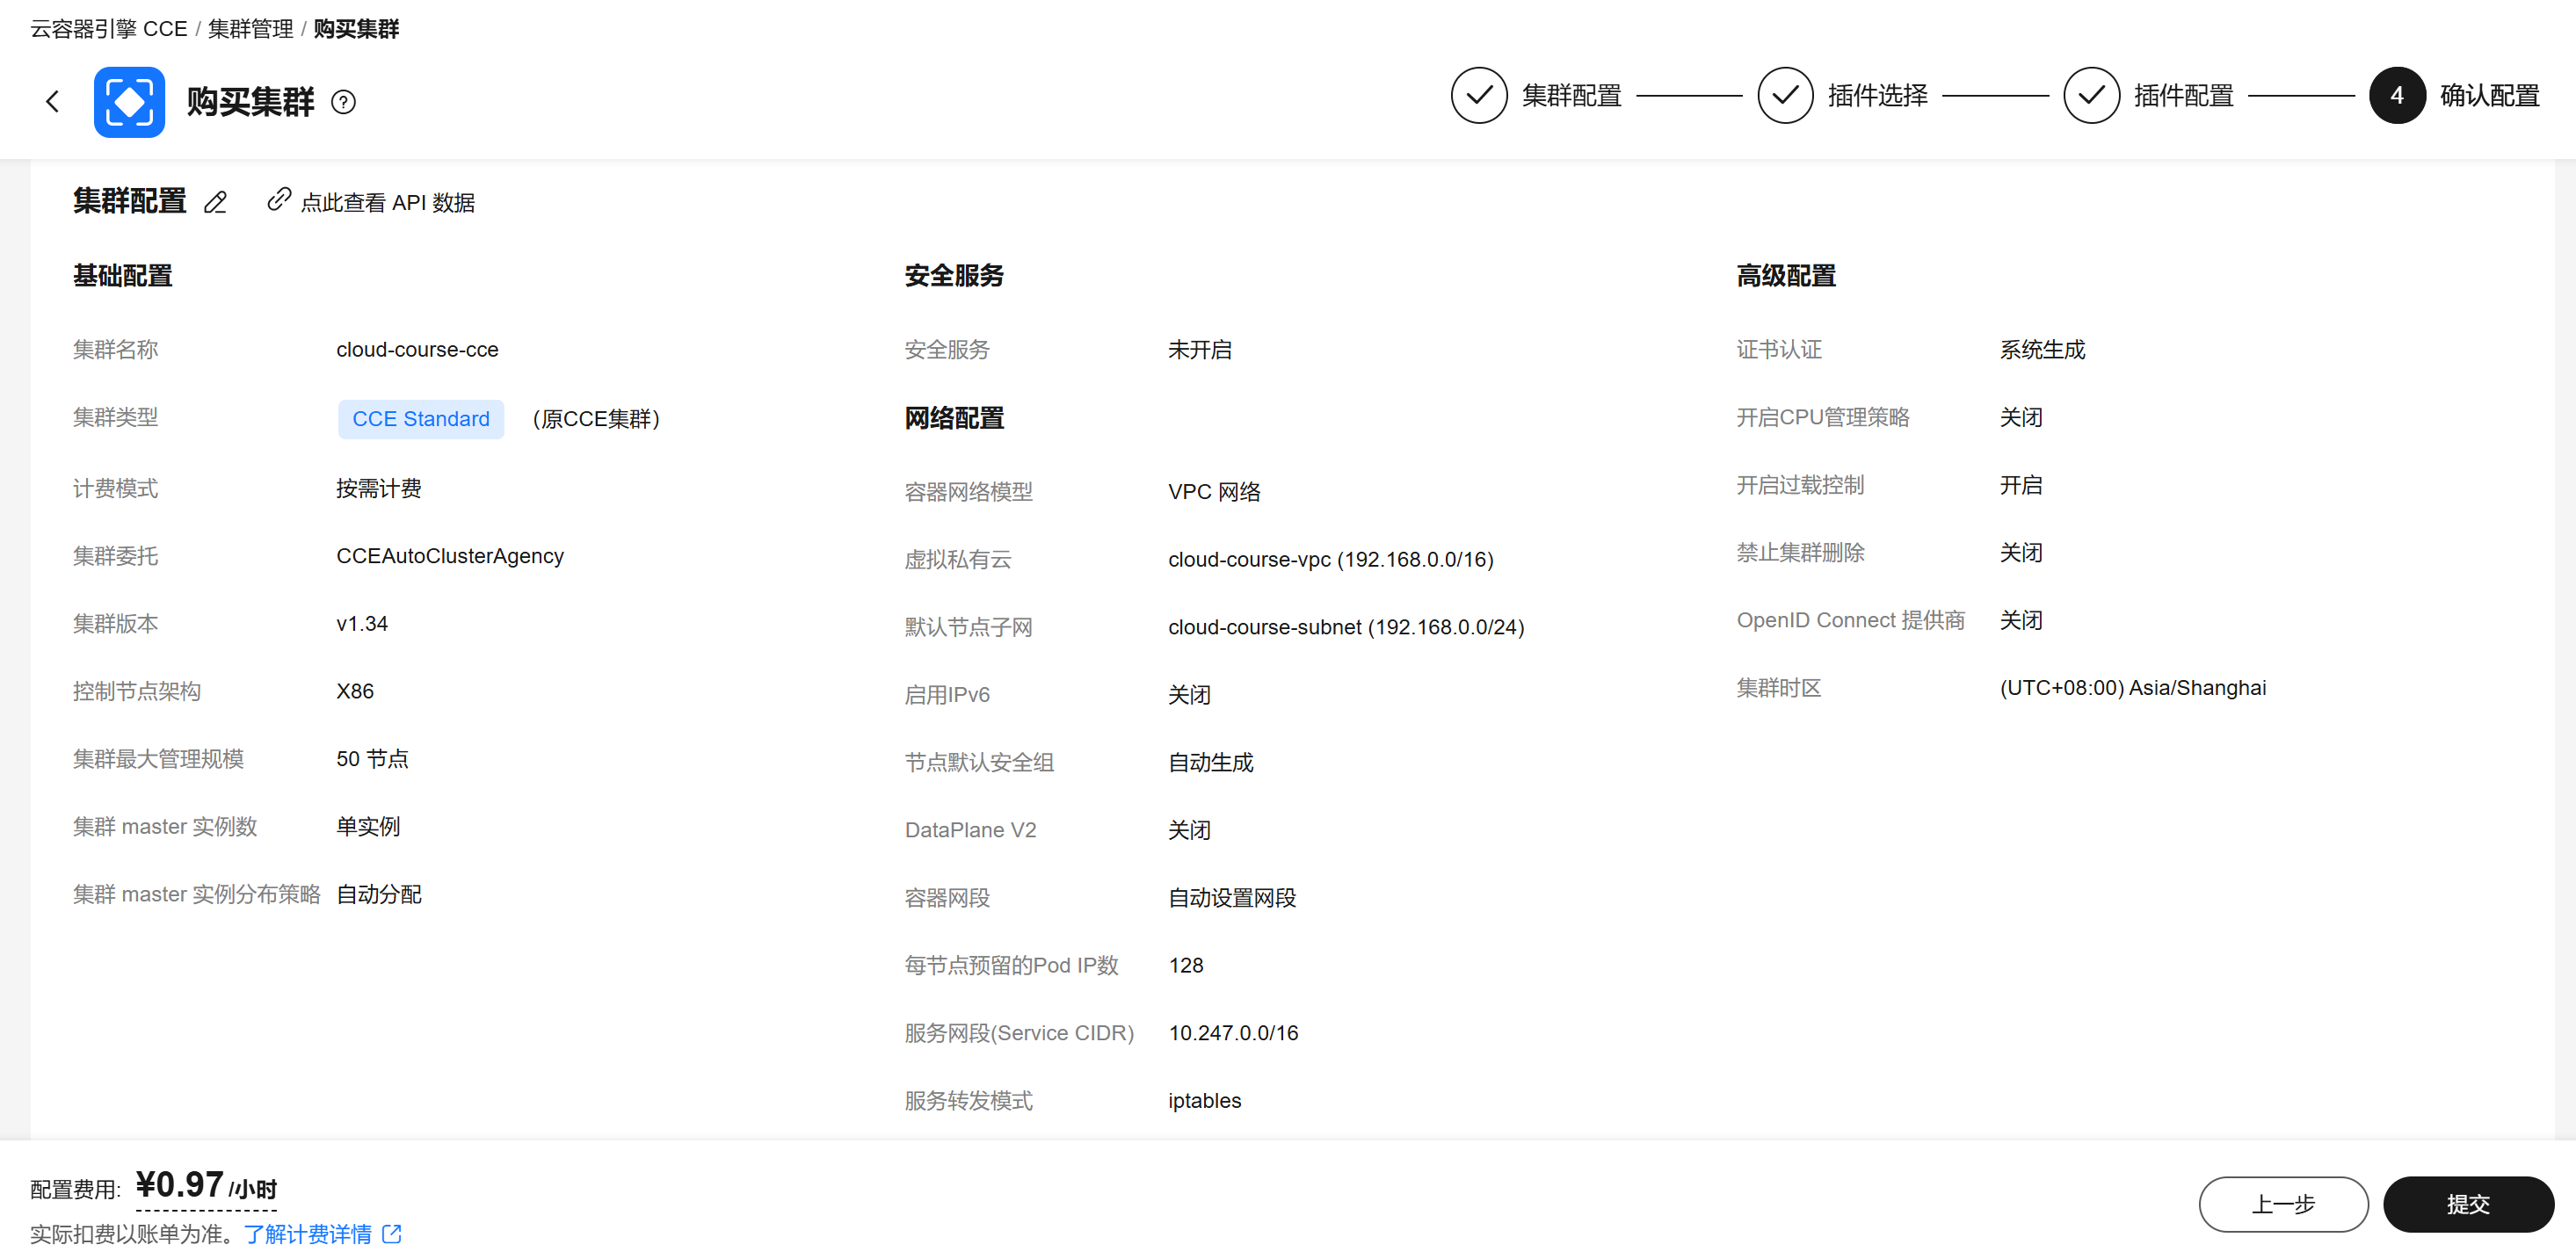
\includegraphics[width=0.80\textwidth]{assets/report_figures/t2/t2-12-cce-final-confirm.png}
  \caption{提交创建 CCE 集群前的最终配置确认截图}
  \label{fig:t2-cce-final-confirm}
\end{figure}

图 \ref{fig:t2-cce-final-confirm} 是提交创建 CCE 集群前的最终确认页面，用来核对集群名称、版本、节点和网络等参数。

\begin{figure}[H]
  \centering
  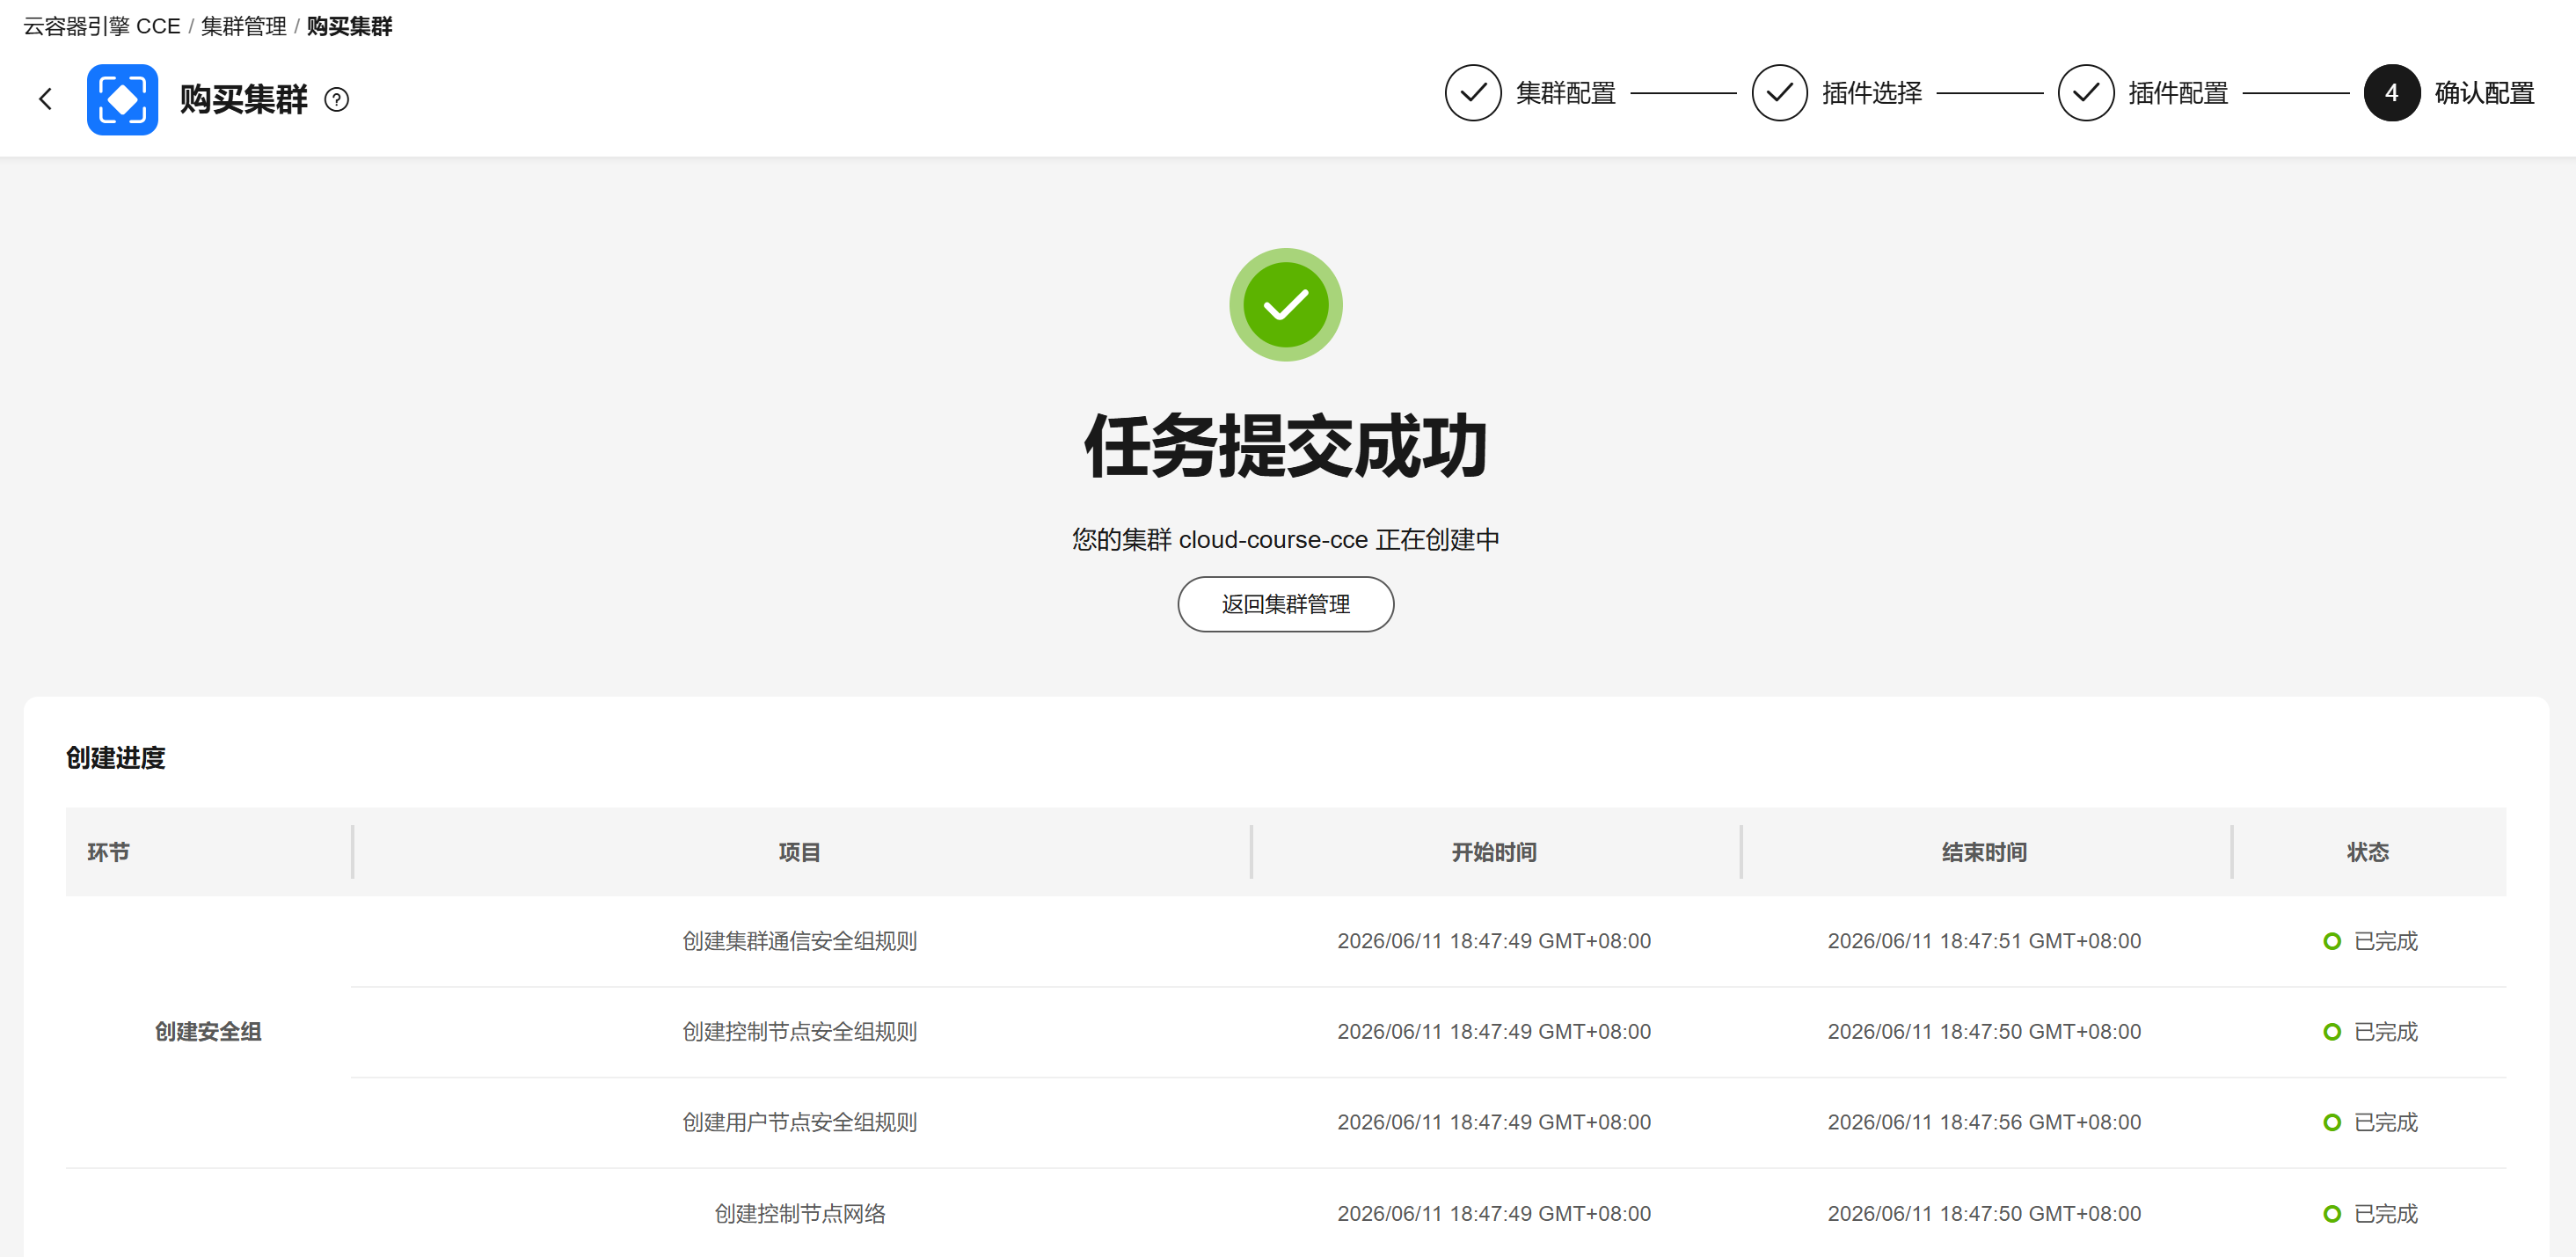
\includegraphics[width=0.92\textwidth]{assets/report_figures/t2/t2-13-cce-creating.png}
  \caption{CCE 集群进入创建中状态截图}
  \label{fig:t2-cce-creating}
\end{figure}

图 \ref{fig:t2-cce-creating} 显示 CCE 集群创建任务已经提交，并进入创建中状态。

\subsubsection{OBS数据存储配置}

OBS 对应 Spark 大数据分析中的数据存储场景，Spark 作业可以通过 \texttt{s3a://} 路径读取对象存储中的文件。本项目的 \texttt{spark/analysis.py} 支持把数据路径作为参数传入，因此既能读取仓库中的本地 \texttt{douban\_movies.csv}，也可以替换为 OBS 路径。当前截图材料中没有单独保存 OBS 控制台页面，因此这里不补放 OBS 截图，Spark 章节只围绕实际脚本和运行结果说明。

OBS 和 CCE 不是直接部署关系。CCE 负责运行 Spark Driver 和 Executor，OBS 只提供数据文件；作业运行时通过 S3A 协议读取数据，再完成 DataFrame 加载、清洗和 SQL 分析。

\subsubsection{ELB负载均衡配置}

ELB 用于对外暴露后端服务。Kubernetes 中的后端 Service 设置为 \texttt{LoadBalancer} 类型后，会绑定华为云 ELB，外部浏览器或 curl 才能访问 \texttt{/api/ping}。T3 验收时主要看公网访问是否返回正常 JSON。

\begin{figure}[H]
  \centering
  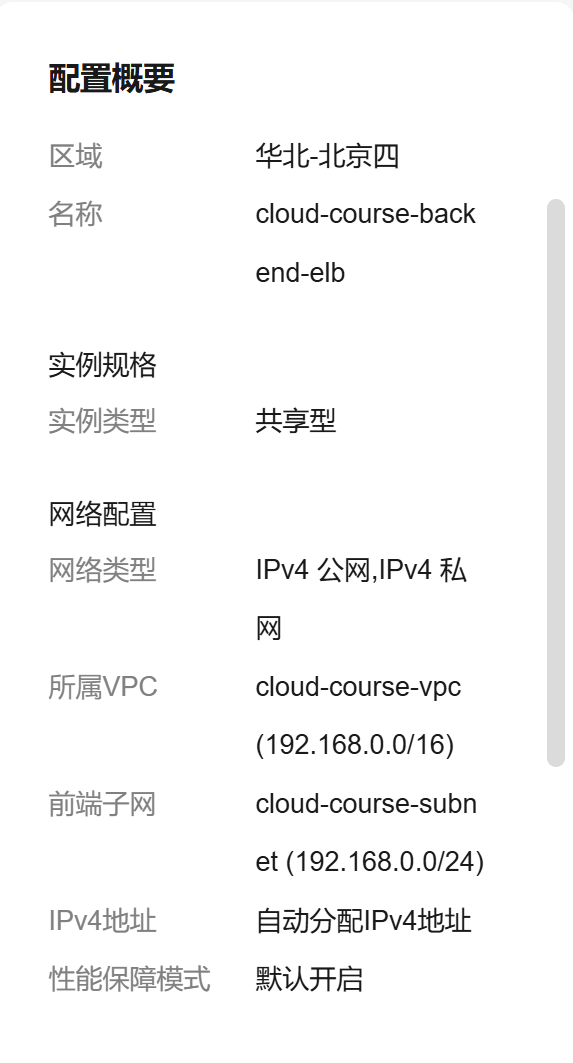
\includegraphics[width=0.65\textwidth]{assets/report_figures/env/env-elb-config.png}
  \caption{共享型公网 ELB 创建配置概要截图}
  \label{fig:env-elb-config}
\end{figure}

图 \ref{fig:env-elb-config} 展示了共享型公网 ELB 的创建配置。该负载均衡器用于后端 \texttt{backend-svc} 的公网访问入口，后续通过 Service 注解将 ELB 与 Kubernetes Service 绑定。

\begin{figure}[H]
  \centering
  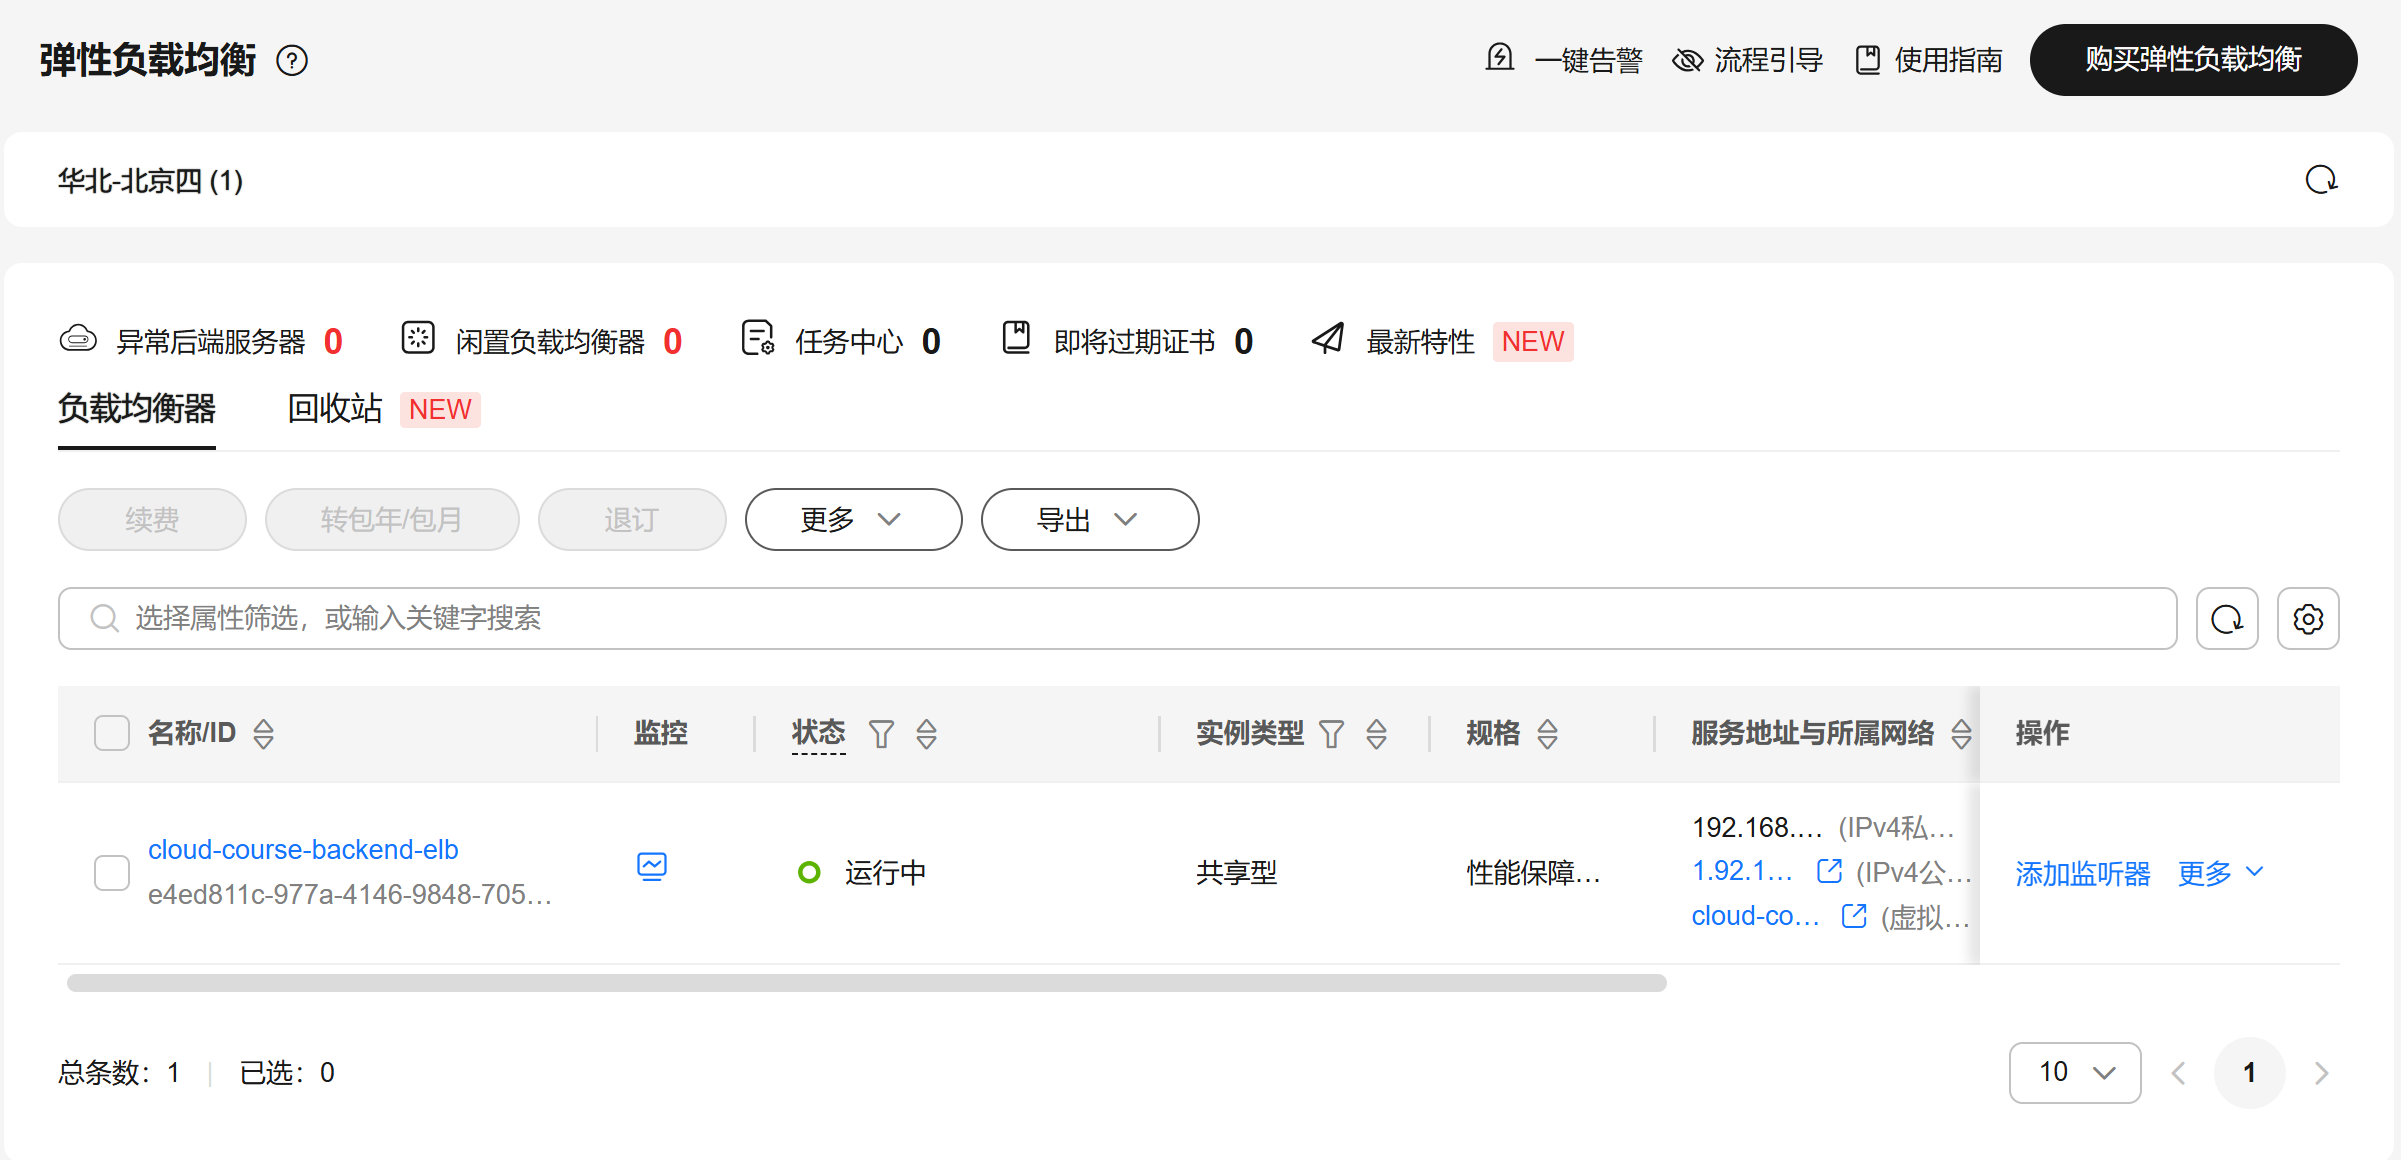
\includegraphics[width=0.92\textwidth]{assets/report_figures/env/env-elb-running.png}
  \caption{ELB 负载均衡器运行中状态截图}
  \label{fig:env-elb-running}
\end{figure}

图 \ref{fig:env-elb-running} 显示 ELB 资源已经创建并处于运行中状态。该状态说明公网负载均衡基础资源可用，为后续通过公网 IP 访问后端接口提供环境条件。

\subsection{Kubernetes集群信息}

T2 主要验收 Kubernetes 集群是否真正可用。集群创建完成后，我们分别在 CCE 控制台和 CloudShell 中检查了节点运行状态、kubectl 连接状态和客户端版本。相关环境参数见表 \ref{tab:k8s-cluster-info}。

\begin{table}[H]
  \centering
  \caption{Kubernetes 集群关键参数}
  \label{tab:k8s-cluster-info}
  \small
  \renewcommand{\arraystretch}{1.22}
  \begin{tabularx}{\textwidth}{>{\raggedright\arraybackslash}p{3.2cm} Y}
    \toprule
    项目 & 内容 \\
    \midrule
    区域 & 华北-北京四 \\
    集群名称 & \texttt{cloud-course-cce} \\
    集群类型 & CCE Standard \\
    计费模式 & 按需计费 \\
    Kubernetes 版本 & v1.34，节点输出中 VERSION 为 \texttt{v1.34.6-r0-34.0.23} \\
    Worker 节点数量 & 2 个 \\
    Worker 节点规格 & \texttt{c9.large.2}，2 vCPU / 4 GiB \\
    操作系统 & Ubuntu 22.04.5 LTS \\
    容器运行时 & containerd \\
    VPC / 子网 & \texttt{cloud-course-vpc} / \texttt{cloud-course-subnet} \\
    \bottomrule
  \end{tabularx}
\end{table}

\subsubsection{集群版本与节点规格}

集群版本和节点规格决定了后续 Kubernetes 资源是否能够稳定运行。本项目选择 v1.34 版本，显著高于任务书要求的 v1.27 下限；节点采用 2 vCPU / 4 GiB 规格，能够满足 Flask 后端、Redis、Nginx 前端以及基础 Spark Operator 验证的课程设计需求，同时控制云资源成本。

\begin{figure}[H]
  \centering
  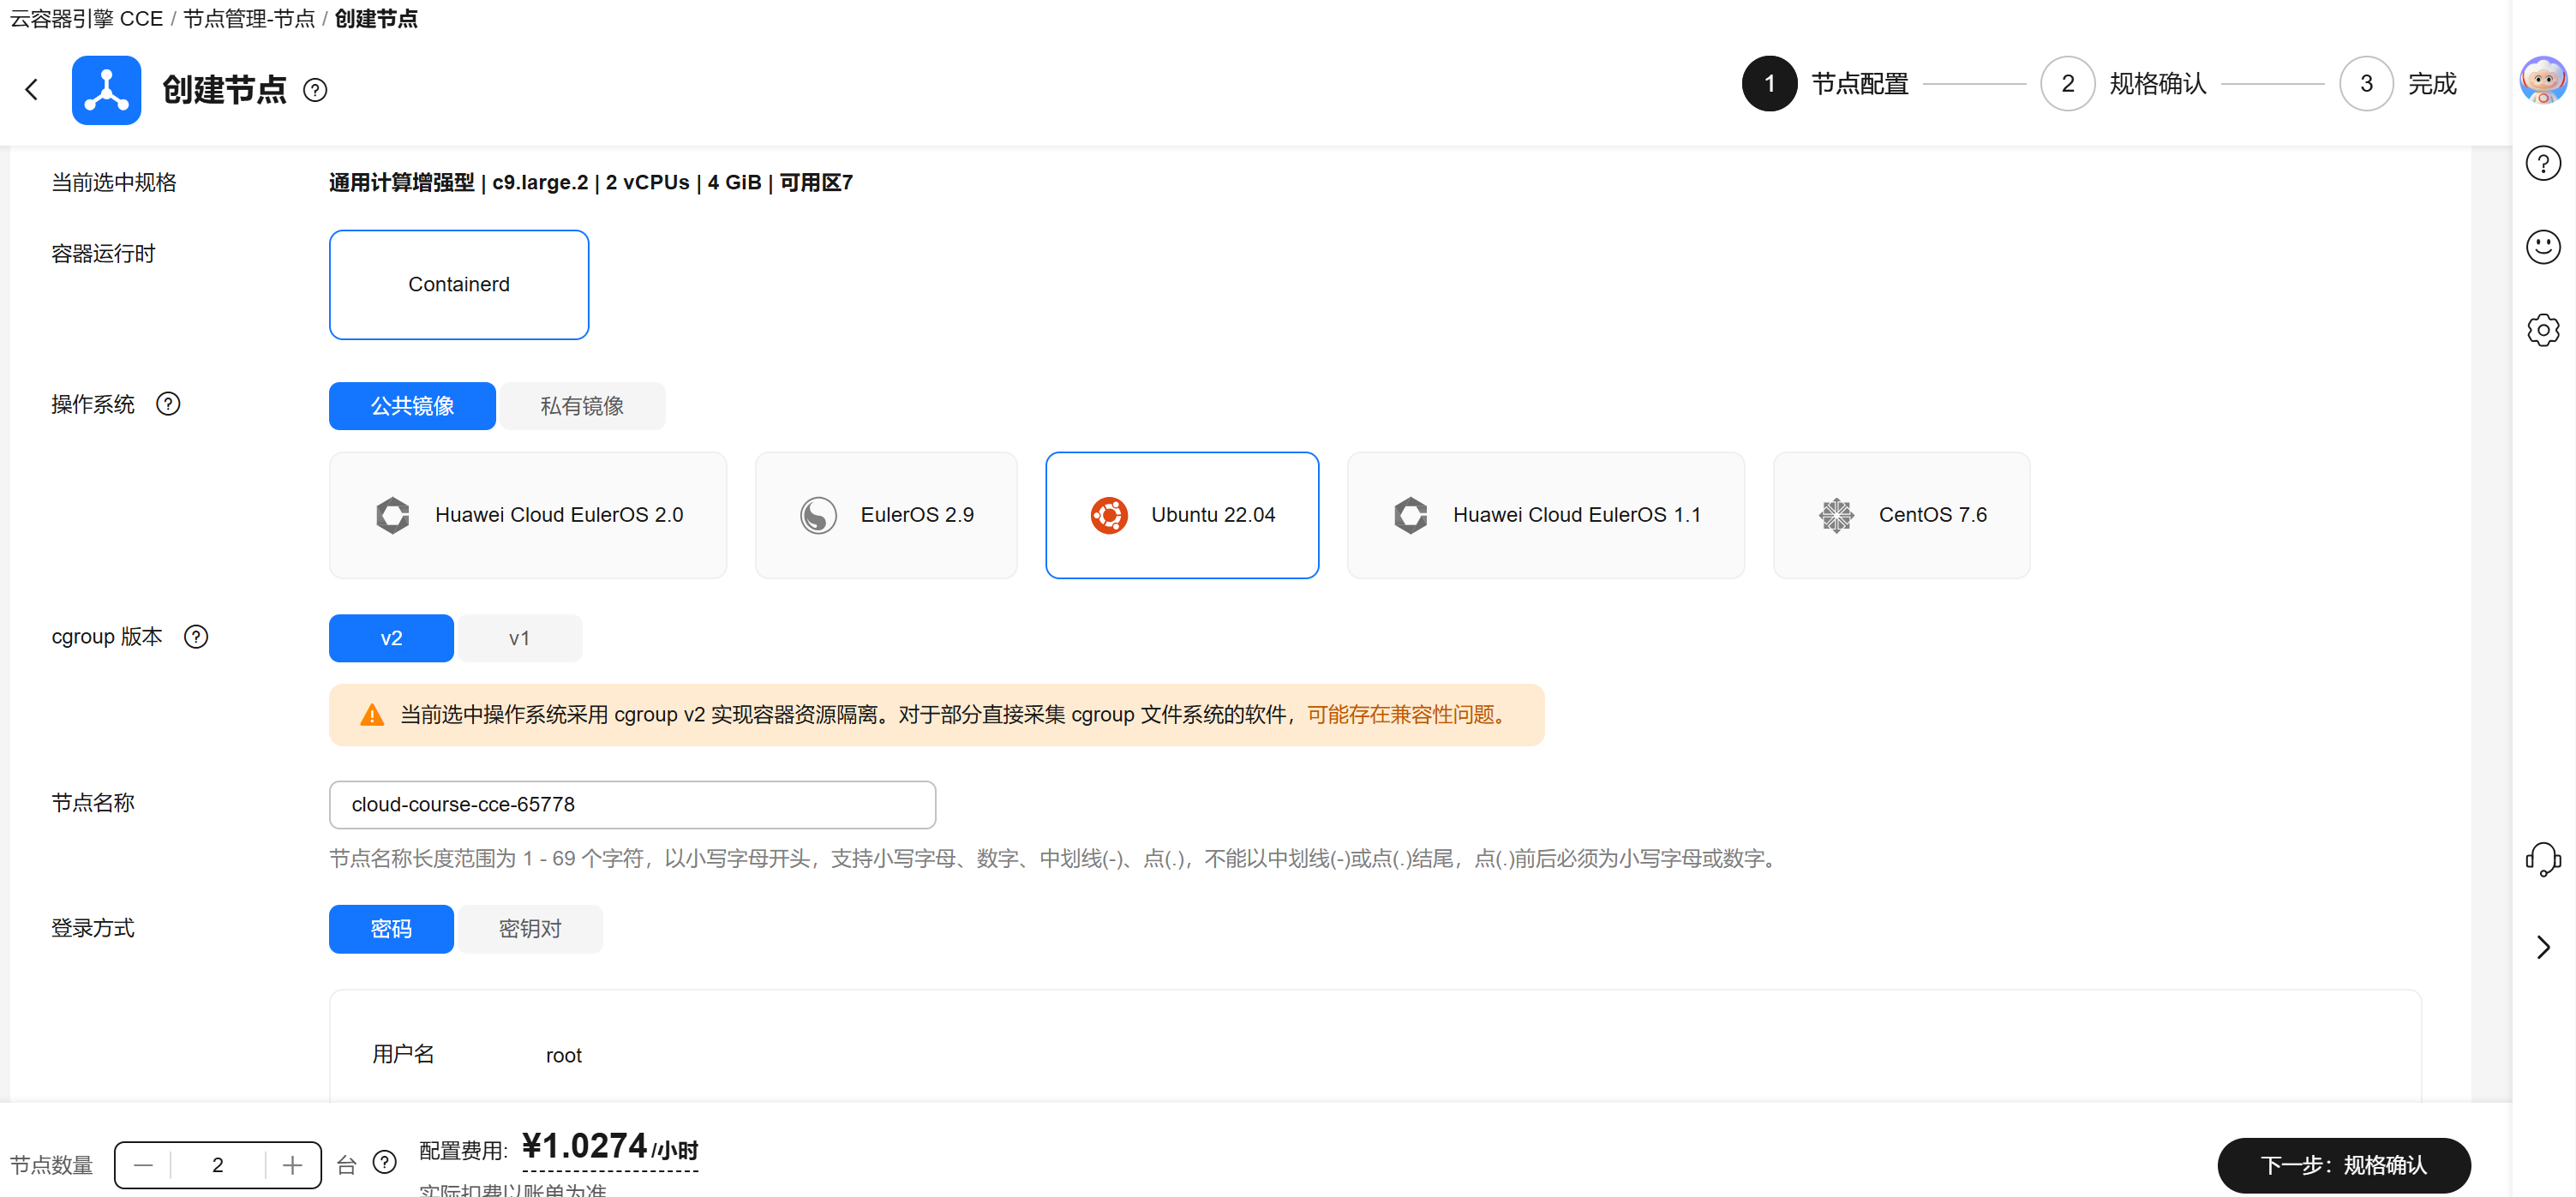
\includegraphics[width=0.92\textwidth]{assets/report_figures/t2/t2-14-worker-config-1.png}
  \caption{创建 Worker 节点时的基础规格配置截图}
  \label{fig:t2-worker-config-1}
\end{figure}

图 \ref{fig:t2-worker-config-1} 记录了 Worker 节点的基础规格配置，可以看出节点规格是按课程设计成本和运行需求手动选择的。

\begin{figure}[H]
  \centering
  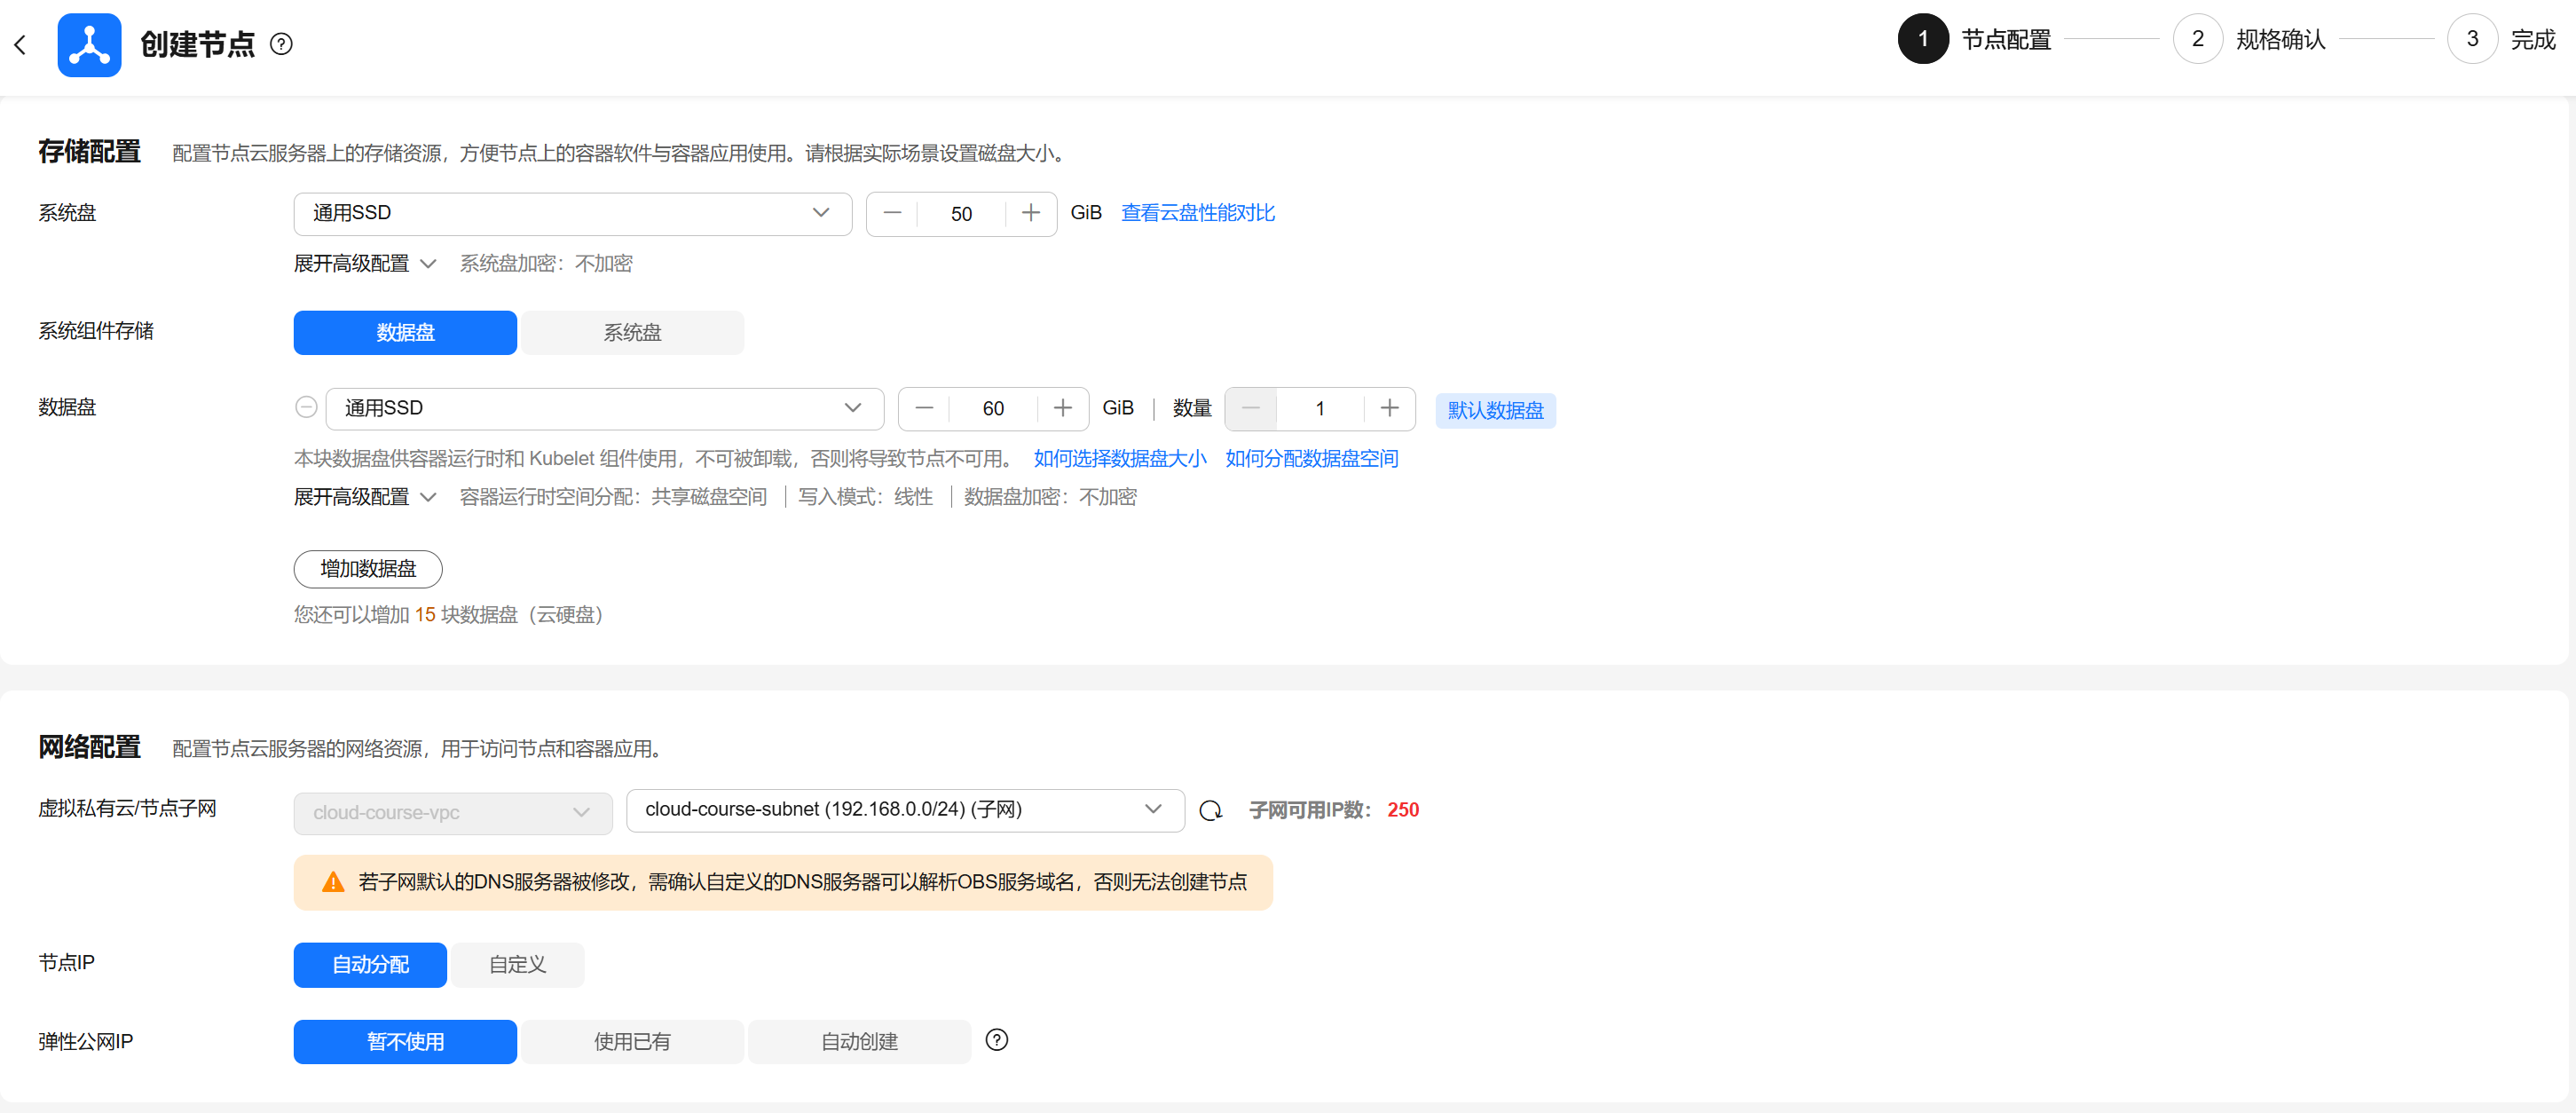
\includegraphics[width=0.92\textwidth]{assets/report_figures/t2/t2-15-worker-config-2.png}
  \caption{创建 Worker 节点时的存储与网络配置截图}
  \label{fig:t2-worker-config-2}
\end{figure}

图 \ref{fig:t2-worker-config-2} 展示了 Worker 节点创建过程中的存储与网络配置。该配置影响节点能否正常加入 VPC、能否创建容器运行环境，以及后续是否能够挂载存储卷。

\begin{figure}[H]
  \centering
  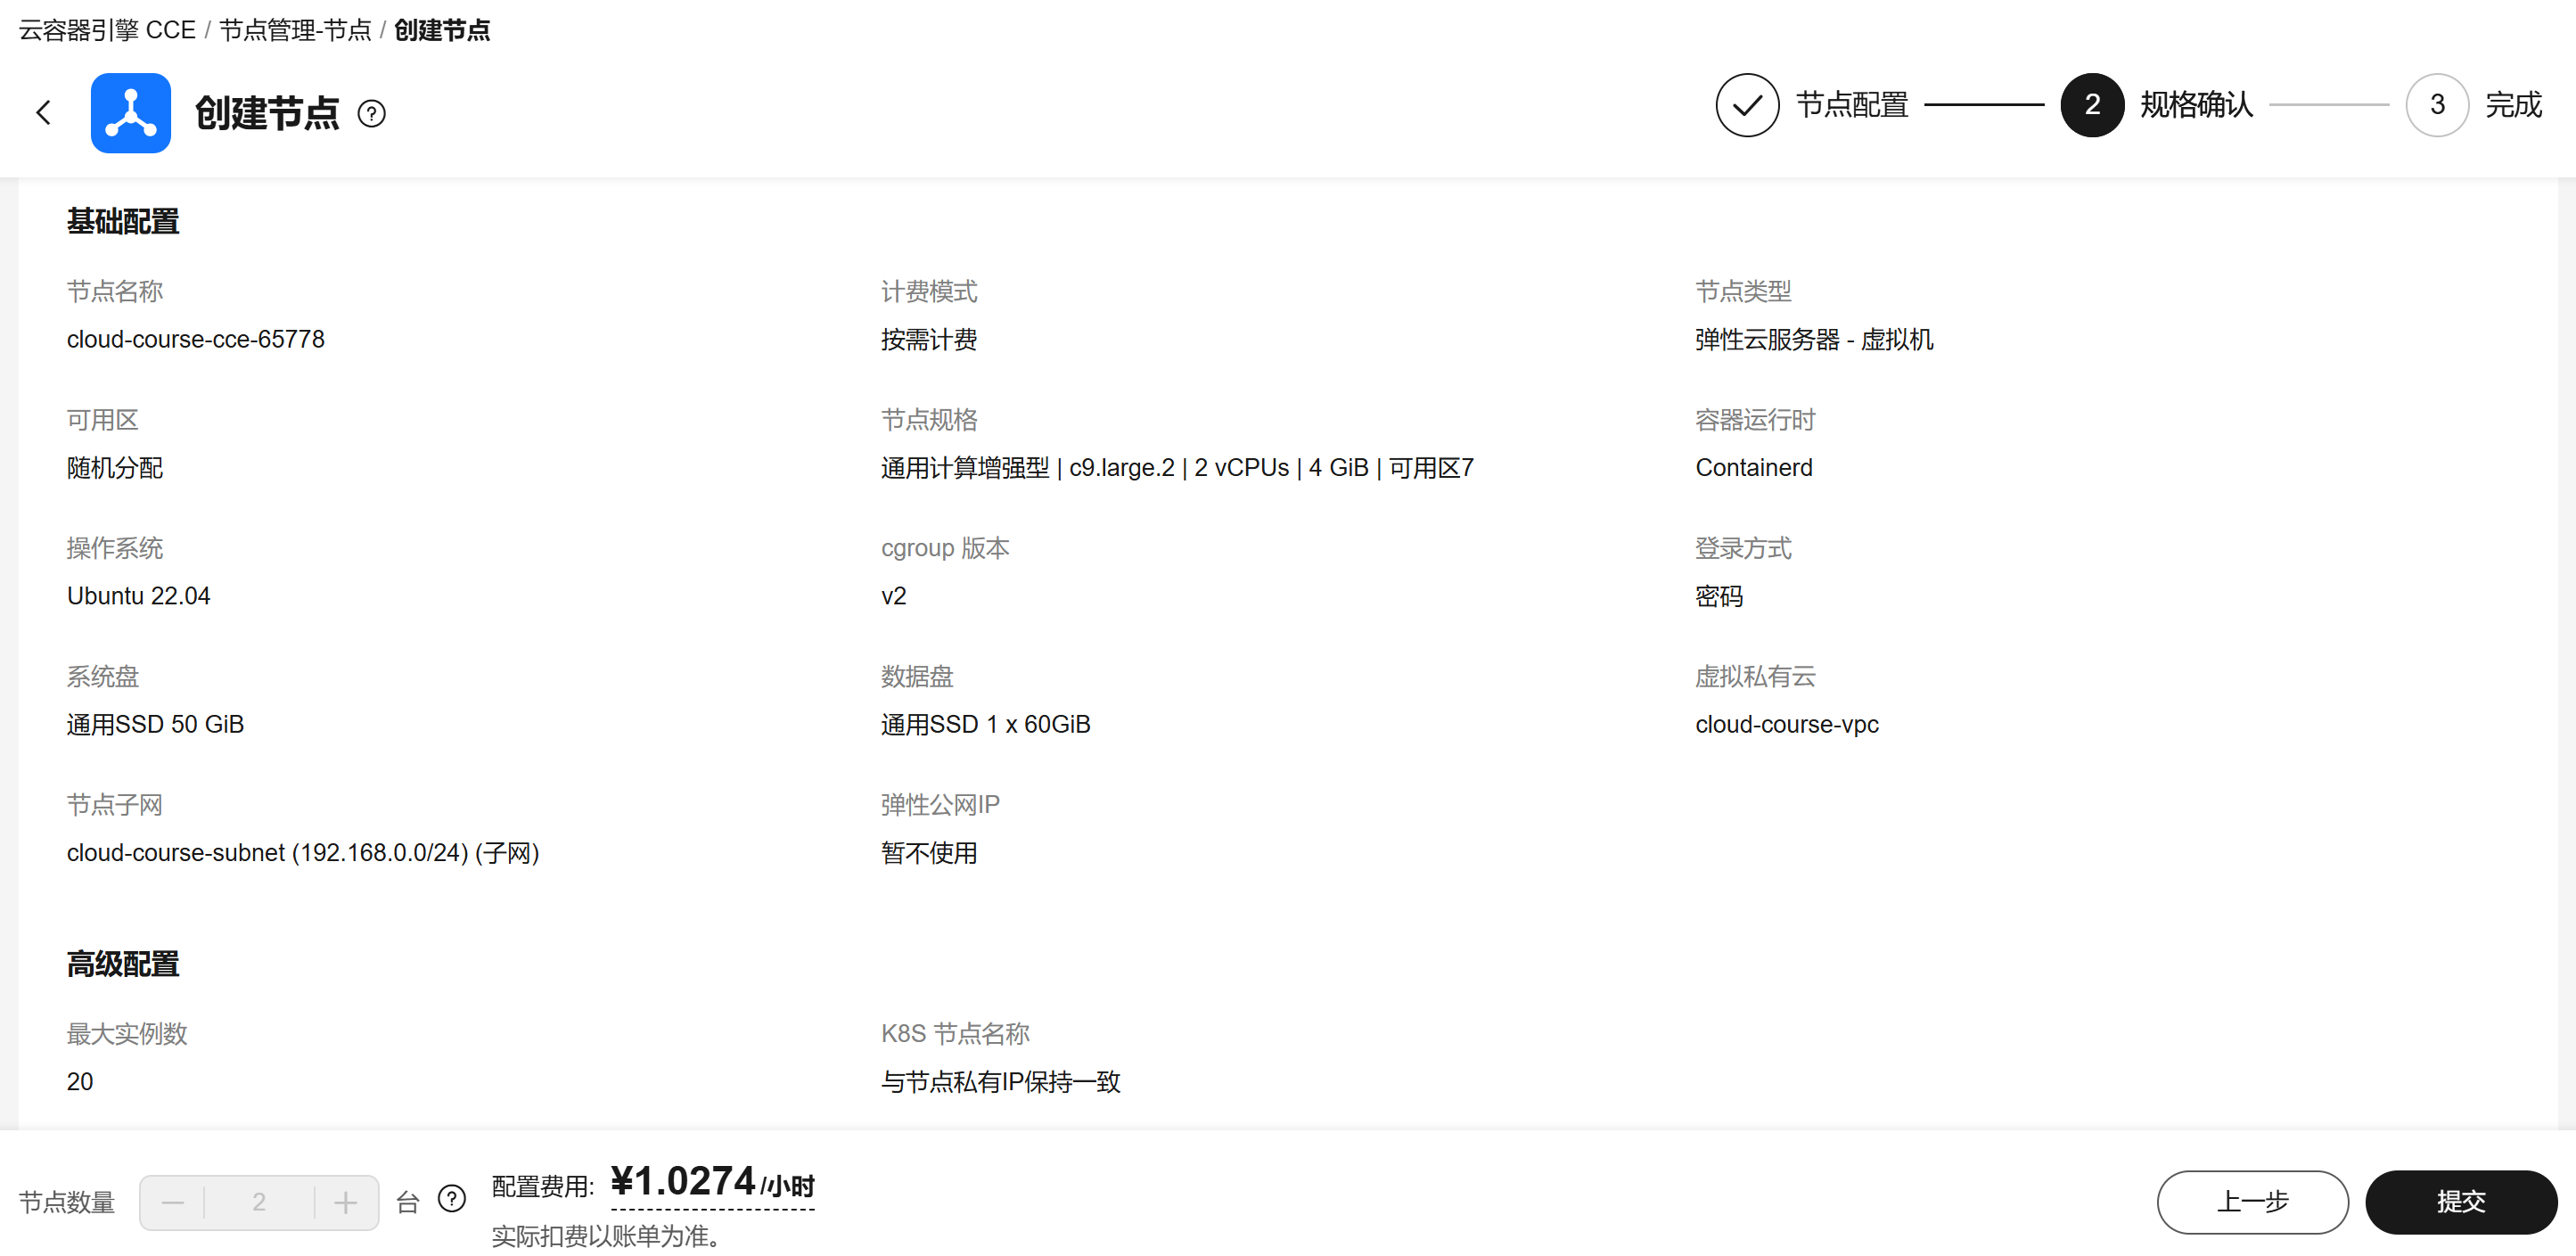
\includegraphics[width=0.92\textwidth]{assets/report_figures/t2/t2-16-worker-confirm.png}
  \caption{Worker 节点规格确认页面截图}
  \label{fig:t2-worker-confirm}
\end{figure}

图 \ref{fig:t2-worker-confirm} 是 Worker 节点规格确认页面，可以看到节点数量和规格。

\begin{figure}[H]
  \centering
  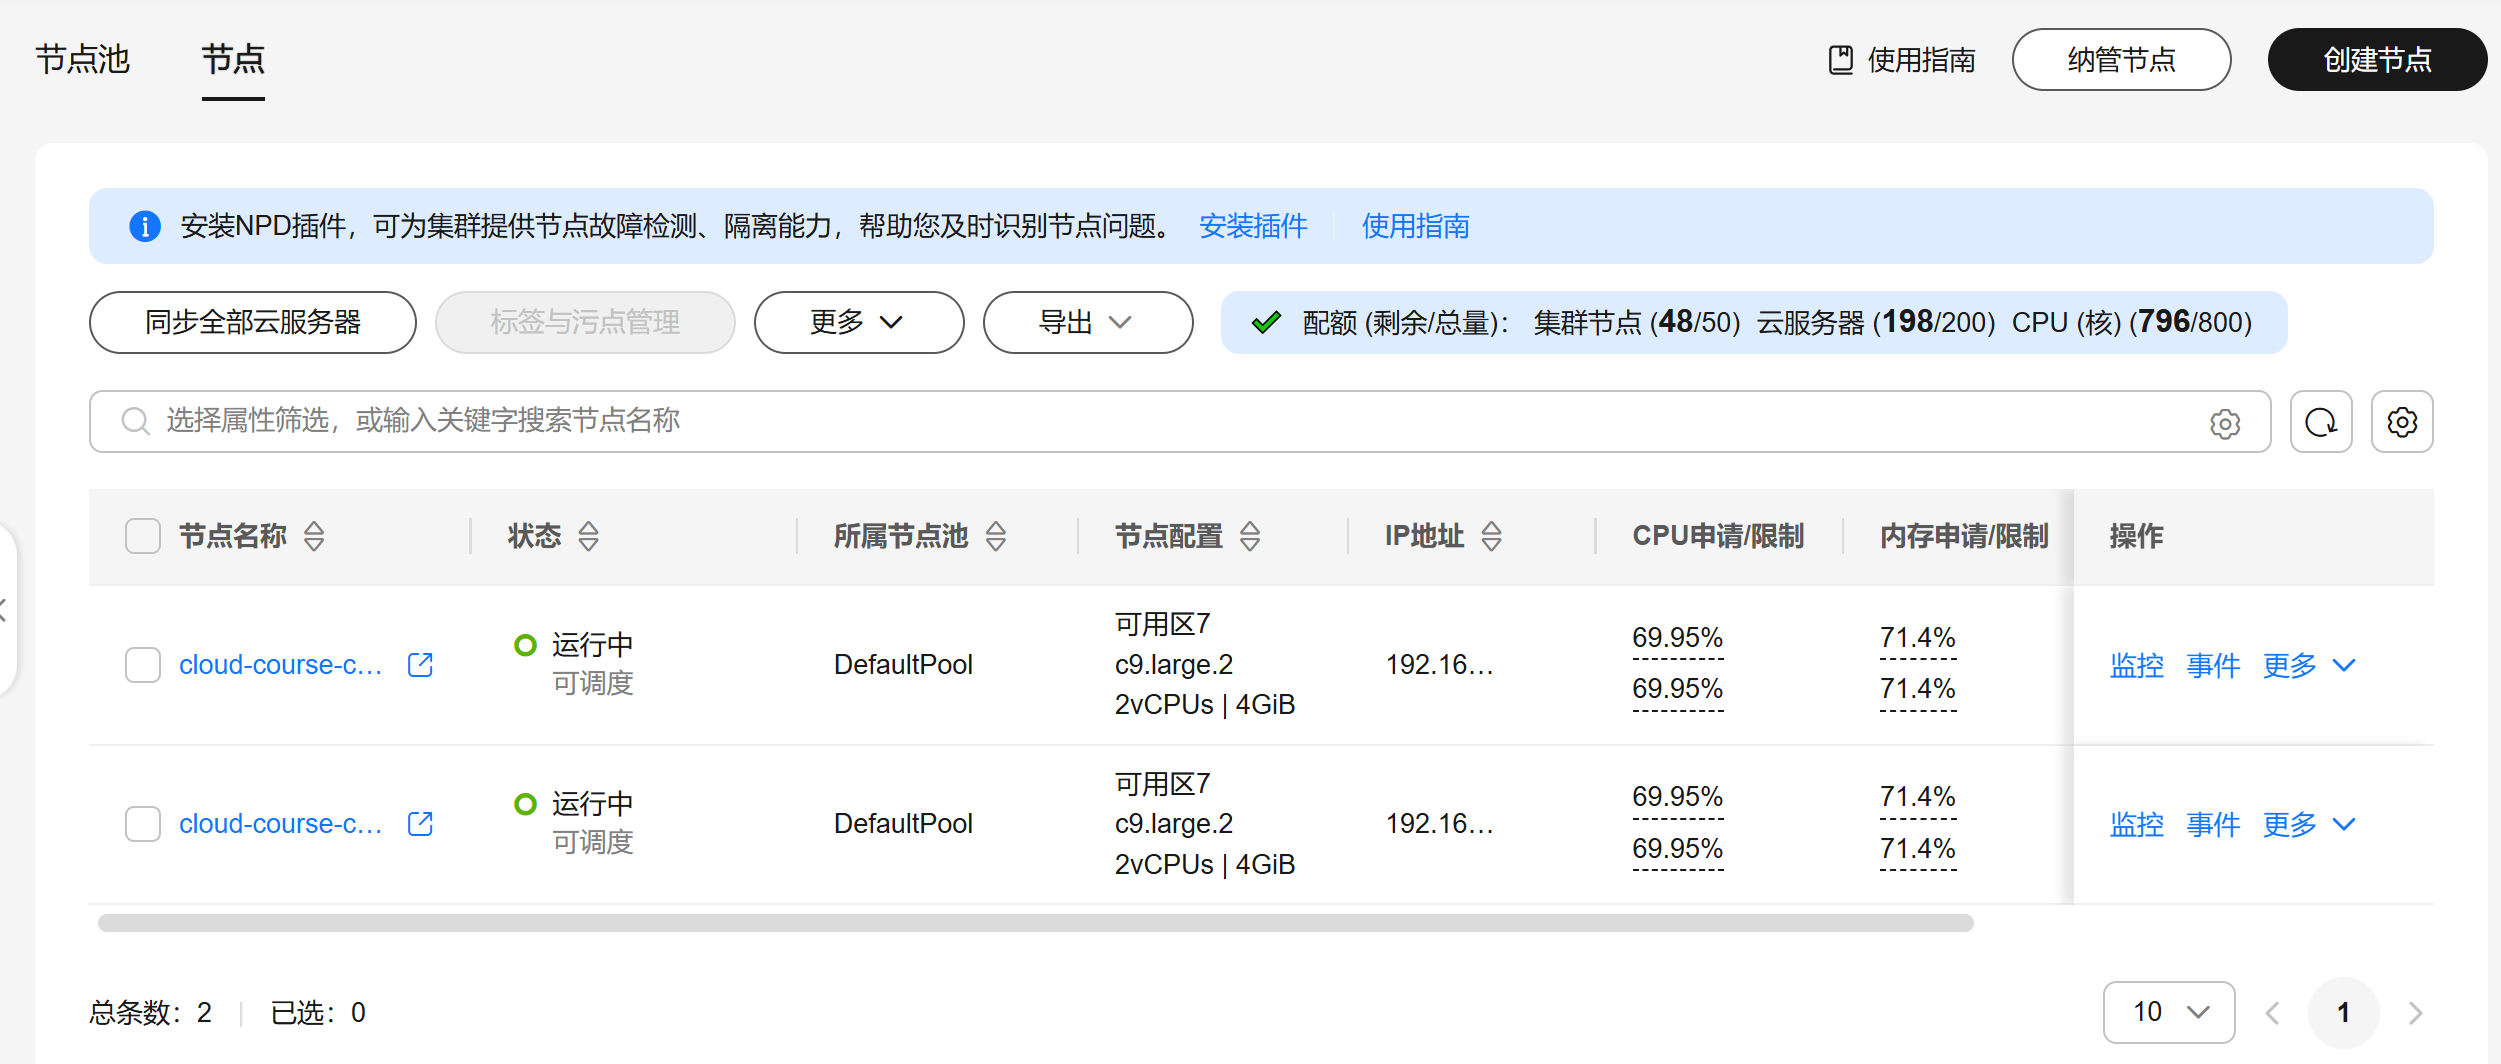
\includegraphics[width=0.92\textwidth]{assets/report_figures/t2/t2-17-worker-running.png}
  \caption{CCE 控制台显示两个 Worker 节点运行中截图}
  \label{fig:t2-worker-running}
\end{figure}

图 \ref{fig:t2-worker-running} 显示 CCE 控制台中两个 Worker 节点处于运行中状态，说明节点已经创建成功。

\subsubsection{kubectl连接与节点状态}

创建集群后，需要配置 kubectl 才能对 Kubernetes 集群执行资源管理操作。本项目使用华为云 CloudShell 配置 kubectl，并通过 \texttt{kubectl get nodes -o wide} 验证两个 Worker 节点均为 Ready。该命令输出同时包含节点名称、状态、角色、版本、内网 IP、操作系统和容器运行时等信息，是任务书 T2 的核心验收截图。

\begin{figure}[H]
  \centering
  {\setlength{\fboxsep}{0pt}\setlength{\fboxrule}{1.2pt}\fcolorbox{red}{white}{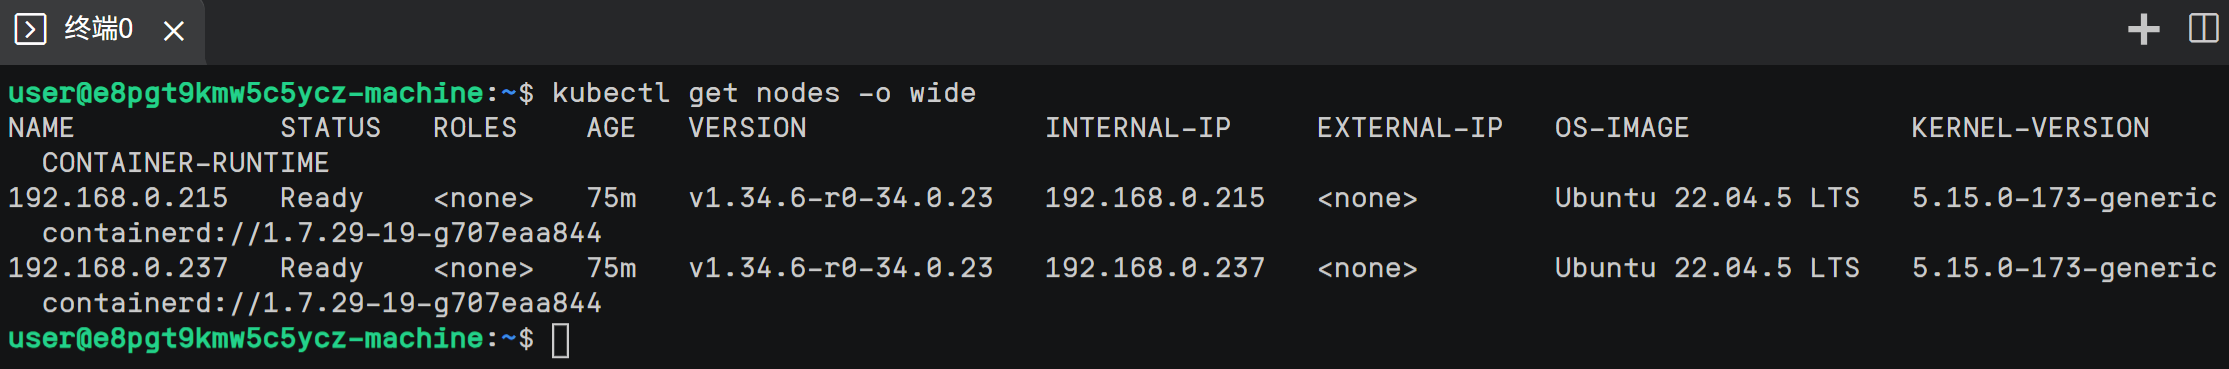
\includegraphics[width=0.88\textwidth]{assets/report_figures/t2/t2-18-nodes-ready.png}}}
  \caption{核心验收：kubectl 查看两个 Worker 节点 Ready 状态截图}
  \label{fig:t2-nodes-ready}
\end{figure}

图 \ref{fig:t2-nodes-ready} 使用红框突出显示核心验收截图。截图中可以看到两个 Worker 节点的 \texttt{STATUS} 均为 \texttt{Ready}，\texttt{VERSION} 列为 \texttt{v1.34.6-r0-34.0.23}，节点内网 IP 分别为 \texttt{192.168.0.215} 和 \texttt{192.168.0.237}。这说明集群节点已经成功加入 Kubernetes，并且版本满足任务书要求。需要说明的是，CCE Worker 节点在 \verb|kubectl get nodes -o wide| 输出中 \texttt{ROLES} 列可能显示为 \verb|<none>|，这是华为云 CCE 托管集群中的常见现象，并不表示节点未就绪；T2 验收以 \texttt{STATUS=Ready} 及 \texttt{VERSION} 列是否满足版本要求为准。

\begin{figure}[H]
  \centering
  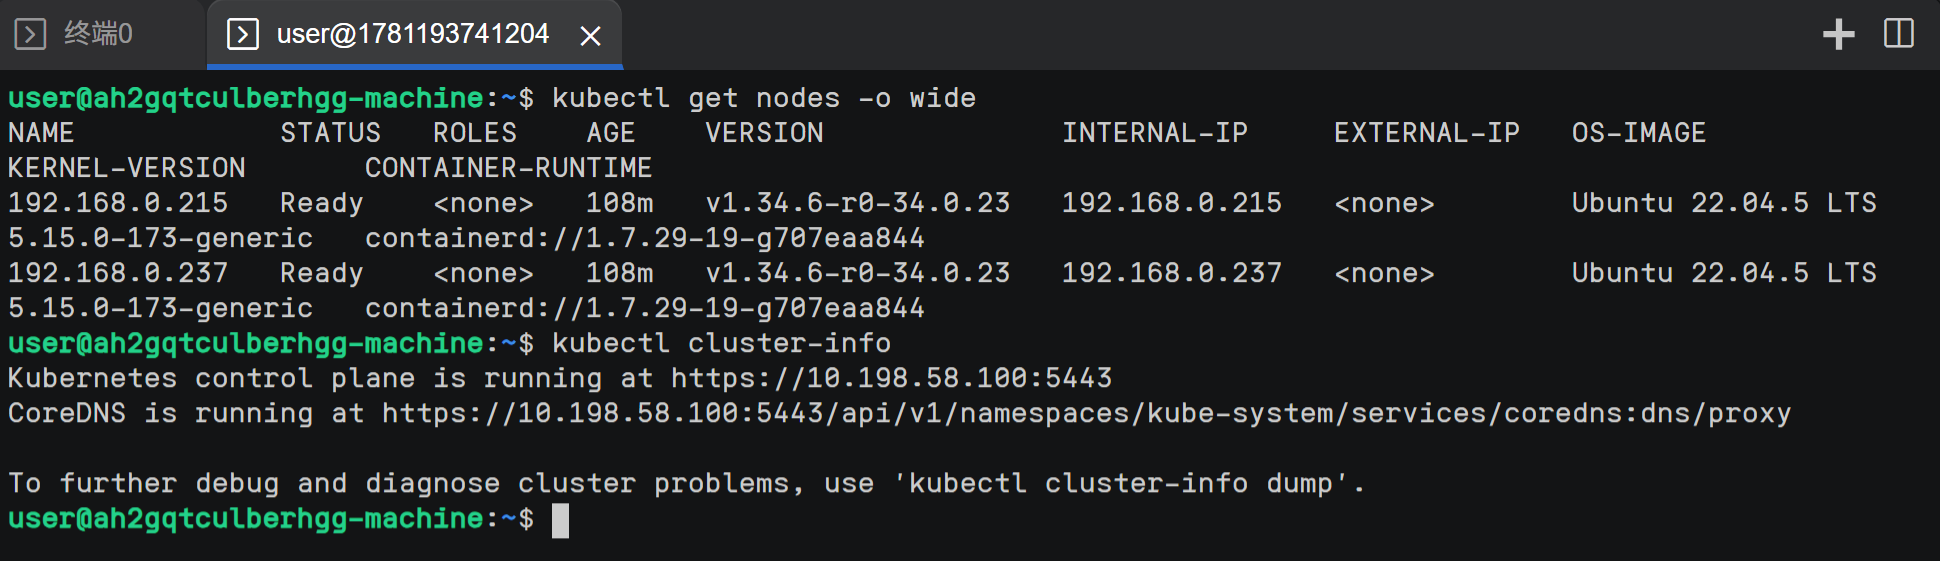
\includegraphics[width=0.92\textwidth]{assets/report_figures/t2/t2-19-cluster-info.png}
  \caption{kubectl cluster-info 连接集群成功截图}
  \label{fig:t2-cluster-info}
\end{figure}

图 \ref{fig:t2-cluster-info} 给出了 \texttt{kubectl cluster-info} 的输出。能看到控制平面地址后，后续才可以继续通过 \texttt{kubectl apply} 部署 YAML 资源。

\begin{figure}[H]
  \centering
  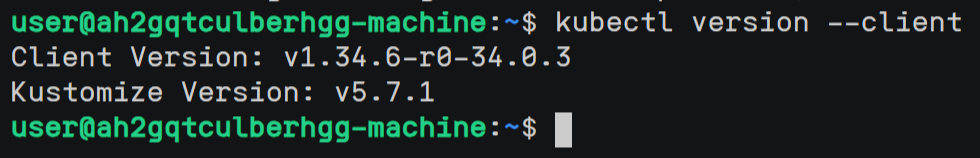
\includegraphics[width=0.92\textwidth]{assets/report_figures/t2/t2-20-kubectl-version.png}
  \caption{kubectl 客户端版本信息截图}
  \label{fig:t2-kubectl-version}
\end{figure}

图 \ref{fig:t2-kubectl-version} 展示了 CloudShell 中 kubectl 客户端版本信息。该截图说明实验环境中 kubectl 工具可用，且后续对 Pod、Service、PVC 和 HPA 的管理均可通过命令行完成。

\subsubsection{命名空间与资源规划}

本项目基础任务主要使用 Kubernetes 的 \texttt{default} 命名空间，便于课程设计验收时统一查看 Pod、Deployment、Service、ConfigMap、Secret、PVC 和 HPA 等资源。后端 Deployment 命名为 \texttt{backend}，Redis Deployment 命名为 \texttt{redis}，前端 Deployment 命名为 \texttt{frontend}；后端 Service 命名为 \texttt{backend-svc}，Redis Service 命名为 \texttt{redis-svc}，前端 Service 命名为 \texttt{frontend-svc}。配置资源方面，后端使用 \texttt{backend-config} 注入 Redis 地址和端口，使用 \texttt{redis-secret} 保存 Redis 密码字段；持久化存储方面，Redis 使用 \texttt{redis-data-pvc} 申请云硬盘存储。

资源命名尽量和任务书中的组件名称保持一致，便于截图核对。敏感配置放入 Secret，普通配置放入 ConfigMap；对外访问只开放后端 LoadBalancer Service，Redis 保持 ClusterIP 内部访问。Spark Operator 和监控系统需要单独命名空间时，在对应实验步骤中再创建。


\section{第一部分：云计算平台搭建}

本章对应课程设计任务书第一部分“云计算平台搭建”，总分 50 分。该部分以“Flask 后端 API + Redis 数据库 + Nginx 前端页面”为应用对象，完成从本地容器化联调到华为云 CCE 集群部署的全过程。报告按照任务书 T1 至 T6 的顺序组织：T1 说明应用容器化与 SWR 镜像推送；T2 说明 CCE 集群搭建与节点 Ready 验证；T3 说明 Kubernetes 资源部署与公网接口访问；T4 说明 Redis PVC 持久化验证；T5 说明 Nginx 配置以 ConfigMap Volume 形式挂载；T6 说明 HPA 弹性伸缩配置及当前仍需补充的验收截图。

\subsection{任务1：应用容器化}

任务 1 的目标是将后端和前端应用分别容器化，并通过本地联调与 SWR 推送证明镜像可运行、可分发。后端采用 Flask 提供 \verb|/api/ping| 接口，并通过 Redis 客户端验证与 Redis 服务的连接状态；前端采用 Nginx 静态页面，页面中包含学生姓名和学号，满足验收识别要求。完成本地构建后，将 \verb|backend:v1| 和 \verb|frontend:v1| 推送至华为云 SWR，为后续 CCE 部署提供镜像来源。

\subsubsection{后端Dockerfile多阶段构建}

后端 Dockerfile 保留了任务书要求的多阶段构建结构。第一阶段基于 \verb|python:3.11-slim| 安装依赖，并将依赖包安装到 \verb|/build/packages|；第二阶段仍使用轻量级 Python 运行时镜像，只复制依赖包和应用代码，并通过 \verb|PYTHONPATH=/app/packages| 指定依赖搜索路径。该结构将依赖安装过程与运行时环境分离，能够减少运行镜像中不必要的构建缓存和工具链内容。

本项目后端依赖文件中包含 \verb|flask==3.0.0|、\verb|redis==5.0.1| 和 \verb|requests==2.31.0|。其中 \verb|requests| 是在基础模板之外加入的自选 Python 包，满足任务书中“至少加入 1 个自选 Python 包”的要求。

\subsubsection{后端依赖包修改与说明}

后端服务依赖 Flask 提供 HTTP API，依赖 Redis Python 客户端连接 Redis 服务，并额外加入 requests 包以体现依赖扩展能力。虽然当前核心接口主要用于健康检查和 Redis 连接验证，但依赖文件采用固定版本号写法，能够减少镜像构建时由于上游包版本变化导致的不确定性。后端容器暴露 5000 端口，启动命令为 \verb|python app.py|，与 Kubernetes Deployment 中的 \verb|containerPort: 5000| 保持一致。

\subsubsection{前端首页学号姓名标识}

前端 Dockerfile 基于 \verb|nginx:1.25-alpine|，将自定义 \verb|nginx.conf| 复制到 \verb|/etc/nginx/conf.d/default.conf|，并将 \verb|static/| 下的静态页面复制到 Nginx 默认网页目录。前端首页 \verb|index.html| 中写入了姓名“李欣纯”和学号“2023116052”，用于课程设计验收时识别提交者身份。该部分满足任务书中“在 Nginx 默认首页中加入本人学号和姓名”的要求。

\reportfig{assets/report_figures/t1/t1-01-docker-desktop.png}{Docker Desktop 正常运行界面}{fig:t1-docker-desktop}

图 \ref{fig:t1-docker-desktop} 显示 Docker Desktop 已正常运行。本地容器化实验依赖 Docker Engine 提供镜像构建和容器运行能力，该截图证明本地构建环境可用。

\subsubsection{Docker Compose本地联调验证}

本地联调使用 \verb|docker compose up -d --build| 同时启动后端与 Redis 服务。Compose 配置中后端通过环境变量读取 Redis 主机、端口和密码，Redis 使用 \verb|redis:7-alpine| 镜像。联调重点不是仅验证容器能够启动，而是验证后端容器能够通过服务名访问 Redis，并且 \verb|/api/ping| 接口能返回正常状态。

\reportfig{assets/report_figures/t1/t1-02-compose-build-up.png}{执行 docker compose up 构建并启动服务截图}{fig:t1-compose-build-up}

图 \ref{fig:t1-compose-build-up} 展示了执行 \verb|docker compose up -d --build| 后服务启动的过程，说明本地镜像能够完成构建并以容器形式运行。

\reportfig{assets/report_figures/t1/t1-03-compose-running.png}{Docker Compose 服务运行状态截图}{fig:t1-compose-running}

图 \ref{fig:t1-compose-running} 展示了本地 Compose 服务运行状态，后端和 Redis 容器均已启动，为接口访问和后端日志验证提供基础。

\reportfig[0.72\textwidth]{assets/report_figures/t1/t1-04-backend-return.png}{本地访问后端接口返回结果截图}{fig:t1-backend-return}

图 \ref{fig:t1-backend-return} 显示本地访问后端接口后获得响应结果，说明 Flask 后端服务能够对外提供 HTTP 接口。

\reportfig[0.72\textwidth]{assets/report_figures/t1/t1-05-status-ok.png}{接口返回 status ok 验证截图}{fig:t1-status-ok}

图 \ref{fig:t1-status-ok} 进一步显示接口返回中包含正常状态信息，说明后端健康检查接口可用，并为后续 CCE 中通过 ELB 访问 \verb|/api/ping| 提供对照。

\reportfig{assets/report_figures/t1/t1-06-backend-logs.png}{后端日志显示收到请求截图}{fig:t1-backend-logs}

图 \ref{fig:t1-backend-logs} 展示后端日志中收到请求的记录。该截图是本地联调的重要证据，说明浏览器或命令行访问确实到达了后端容器，而不仅是静态页面或缓存结果。

\subsubsection{SWR镜像推送与镜像Tag验证}

本地联调通过后，将后端和前端镜像分别标记为 \verb|v1|，并推送至华为云 SWR。镜像推送完成后，CCE Deployment 中即可引用 SWR 镜像地址创建 Pod。SWR 推送过程是从本地实验过渡到云端部署的关键步骤，若镜像未正确推送或标签不一致，后续 Kubernetes Pod 将无法拉取业务镜像。

\reportfig{assets/report_figures/t1/t1-07-backend-tag.png}{后端镜像标记为 v1 截图}{fig:t1-backend-tag}

图 \ref{fig:t1-backend-tag} 展示后端镜像完成 \verb|v1| 标签标记。该标签与后续 Deployment 中引用的镜像标签保持一致。

\reportfig{assets/report_figures/t1/t1-08-frontend-tag.png}{前端镜像标记为 v1 截图}{fig:t1-frontend-tag}

图 \ref{fig:t1-frontend-tag} 展示前端镜像完成 \verb|v1| 标签标记，说明前端静态页面和 Nginx 配置已经形成可推送的镜像版本。

\reportfig{assets/report_figures/t1/t1-09-swr-list.png}{SWR 控制台镜像列表截图}{fig:t1-swr-list}

图 \ref{fig:t1-swr-list} 显示 SWR 控制台中已经存在相关镜像及 Tag。该截图满足任务书中“SWR 控制台截图需含镜像名称和 Tag”的验收要求。

\subsection{任务2：CCE集群搭建}

任务 2 要求在华为云 CCE 控制台创建 Kubernetes 集群，并配置 kubectl，使至少两个 Worker 节点处于 Ready 状态。本项目已在第二章对 CCE、VPC、子网、Worker 节点、插件和 kubectl 连接过程进行了完整说明，并插入了 T2 的全部环境截图。本节从第一部分评分角度简要归纳验收结论。

\subsubsection{CCE集群创建过程}

本项目在华为云华北-北京四区域创建 CCE Standard 集群 \verb|cloud-course-cce|，并配套创建 VPC \verb|cloud-course-vpc| 和子网 \verb|cloud-course-subnet|。集群创建时保留 CCE 容器网络、CoreDNS 和 Everest 存储等默认必要插件，为后续服务发现、Pod 网络通信和 PVC 挂载提供基础能力。

\subsubsection{Worker节点Ready状态验证}

集群创建完成后，使用 CloudShell 配置 kubectl，并执行 \verb|kubectl get nodes -o wide|。第二章图 \ref{fig:t2-nodes-ready} 中可以看到两个 Worker 节点均处于 \verb|Ready| 状态，说明节点已经成功加入集群并可承载业务 Pod。

\subsubsection{Kubernetes版本要求验证}

节点输出中的 Kubernetes 版本为 \verb|v1.34.6-r0-34.0.23|，高于任务书要求的 1.27 版本下限。节点操作系统为 Ubuntu 22.04.5 LTS，容器运行时为 containerd。由此可见，T2 在节点数量、节点状态和版本要求三个方面均满足验收标准。

\subsection{任务3：应用部署}

任务 3 的目标是将任务 1 中完成的容器镜像部署到 CCE 集群中，并通过 Kubernetes 资源完成服务编排、配置注入、敏感信息管理和公网暴露。本项目部署的主要资源包括 \verb|backend| Deployment、\verb|redis| Deployment、\verb|frontend| Deployment、\verb|backend-svc| LoadBalancer Service、\verb|redis-svc| ClusterIP Service、\verb|backend-config| ConfigMap 和 \verb|redis-secret| Secret。

\reportfig{assets/report_figures/t3/t3-09-before-state.png}{T3 部署前集群资源状态截图}{fig:t3-before-state}

图 \ref{fig:t3-before-state} 展示应用部署前集群资源状态，用于说明部署操作是在已有 CCE 集群基础上进行，而非仅展示最终结果。

\reportfig{assets/report_figures/t3/t3-10-yaml-ready.png}{CloudShell 中 T3 YAML 文件准备完成截图}{fig:t3-yaml-ready}

图 \ref{fig:t3-yaml-ready} 显示 CloudShell 中已准备好 T3 所需 YAML 文件。该截图证明部署使用的是可追溯的 Kubernetes 配置文件。

\reportfig{assets/report_figures/t3/t3-11-yaml-check.png}{T3 关键 YAML 配置检查截图}{fig:t3-yaml-check}

图 \ref{fig:t3-yaml-check} 展示了 T3 关键 YAML 配置检查结果，包括副本数、Service 类型、ELB 注解和 Redis 配置等内容，能够体现部署前对配置正确性的核对。

\reportfig{assets/report_figures/t3/t3-01-yaml-apply.png}{应用 Kubernetes YAML 资源成功截图}{fig:t3-yaml-apply}

图 \ref{fig:t3-yaml-apply} 显示 Kubernetes YAML 资源已成功应用到集群中，是 T3 从配置文件进入实际集群状态的直接证据。

\subsubsection{后端Deployment配置}

后端 Deployment 名称为 \verb|backend|，副本数设置为 2，符合任务书“后端副本数=2”的要求。容器镜像来自华为云 SWR，容器端口为 5000，并配置了资源请求与限制，使调度器能够根据 CPU 和内存需求安排 Pod。后端通过 \verb|configMapRef| 引入 Redis 地址和端口，通过 \verb|secretKeyRef| 引入 Redis 密码字段，实现配置与代码分离。

\subsubsection{Redis Deployment配置}

Redis Deployment 名称为 \verb|redis|，副本数为 1，镜像为 \verb|redis:7-alpine|。Redis 作为后端服务依赖的内部数据组件，不直接暴露公网访问入口，而是通过 ClusterIP Service 在集群内部提供访问。后续 T4 中 Redis 还会挂载 PVC，将数据目录持久化到云硬盘。

\subsubsection{后端LoadBalancer Service配置}

后端 Service 名称为 \verb|backend-svc|，类型为 \verb|LoadBalancer|，对外暴露 80 端口，并转发到后端容器的 5000 端口。由于华为云 CCE 中 LoadBalancer Service 需要与 ELB 资源绑定，本项目在遇到 \verb|EXTERNAL-IP| 长时间 \verb|<pending>| 后，创建共享型公网 ELB 并通过 Service 注解绑定，从而获得公网 IP。

\reportfig{assets/report_figures/t3/t3-12-pending-problem.png}{backend-svc 外部 IP 持续 Pending 问题截图}{fig:t3-pending-problem}

图 \ref{fig:t3-pending-problem} 记录了 \verb|backend-svc| 初始外部 IP 处于 \verb|<pending>| 的问题现象。该截图用于说明部署过程中存在真实排错过程，而不是简单套用模板。

\reportfig{assets/report_figures/t3/t3-04-services-elb.png}{Service 列表与 ELB 公网 IP 截图}{fig:t3-services-elb}

图 \ref{fig:t3-services-elb} 显示 \verb|backend-svc| 为 \verb|LoadBalancer| 类型，并已经获得 ELB 公网 IP。该截图说明公网访问入口已经建立。

\subsubsection{Redis ClusterIP Service配置}

Redis Service 名称为 \verb|redis-svc|，类型为 \verb|ClusterIP|，端口为 6379。该设计符合最小暴露原则：Redis 只需要被后端 Pod 访问，不需要直接暴露到公网。后端通过 ConfigMap 中的 \verb|REDIS_HOST=redis-svc| 和 \verb|REDIS_PORT=6379| 访问 Redis 服务，体现 Kubernetes Service 名称解析和内部服务发现机制。

\subsubsection{ConfigMap与Secret配置}

本项目使用 \verb|backend-config| 保存非敏感配置，包括 Redis 主机名、端口和应用运行环境；使用 \verb|redis-secret| 保存敏感密码字段。ConfigMap 与 Secret 分别承担非敏感配置和敏感配置管理职责，能够避免将环境相关配置写死在镜像中，也符合云原生应用“配置外置化”的实践原则。

\reportfig{assets/report_figures/t3/t3-08-config-secret.png}{ConfigMap 与 Secret 资源存在截图}{fig:t3-config-secret}

图 \ref{fig:t3-config-secret} 显示 \verb|backend-config|、\verb|frontend-nginx-config| 和 \verb|redis-secret| 等资源已经存在，说明配置资源已经部署到集群中。

\subsubsection{Pod运行状态与接口访问验证}

应用部署完成后，通过 \verb|kubectl get pods|、浏览器访问和 curl 命令进行验证。核心验收点包括所有 Pod 处于 Running 状态，以及通过 ELB 公网 IP 访问 \verb|/api/ping| 能够返回正常 JSON 结果。

\reportfig{assets/report_figures/t3/t3-02-pods-running.png}{核心验收：Pod 全部 Running 状态截图}{fig:t3-pods-running}

图 \ref{fig:t3-pods-running} 显示 backend、frontend 和 redis 相关 Pod 均处于 Running 状态，其中后端有两个副本，符合任务书要求。

\reportfig{assets/report_figures/t3/t3-03-deployments.png}{Deployment 副本数与镜像信息截图}{fig:t3-deployments}

图 \ref{fig:t3-deployments} 展示了 Deployment 副本数和镜像信息，可以看到 backend、frontend 和 redis 的部署状态以及镜像来源。

\reportfig[0.72\textwidth]{assets/report_figures/t3/t3-05-browser-ping.png}{浏览器访问 api/ping 返回正常截图}{fig:t3-browser-ping}

图 \ref{fig:t3-browser-ping} 显示通过浏览器访问公网入口后，后端接口返回正常，说明 ELB 到后端 Service 的访问路径可用。

\reportfig[0.72\textwidth]{assets/report_figures/t3/t3-06-curl-ping.png}{curl 访问 api/ping 返回正常截图}{fig:t3-curl-ping}

图 \ref{fig:t3-curl-ping} 显示命令行访问 \verb|/api/ping| 返回 \verb|{"redis":"connected","status":"ok"}|。该结果不仅说明后端接口可访问，也说明后端能够连接 Redis。

\reportfig{assets/report_figures/t3/t3-07-backend-logs.png}{后端 Pod 日志收到请求截图}{fig:t3-backend-logs}

图 \ref{fig:t3-backend-logs} 展示后端 Pod 日志收到请求并返回 200 状态码，进一步证明公网访问请求最终到达后端业务容器。

\subsection{任务4：持久化存储}

任务 4 要求为 Redis 配置 PVC，并验证 Redis Pod 删除重建后数据不丢失。本项目创建 \verb|redis-data-pvc|，使用华为云 \verb|csi-disk| StorageClass 申请 10Gi 云硬盘，并在 Redis Deployment 中将 PVC 挂载到容器内 \verb|/data| 目录。随后通过写入 \verb|testkey=hello|、删除 Redis Pod、等待新 Pod 重建、再次查询 \verb|testkey| 的方式验证持久化效果。

\reportfig{assets/report_figures/t4/t4-00-apply.png}{Redis PVC 与 Deployment 创建成功截图}{fig:t4-apply}

图 \ref{fig:t4-apply} 显示 Redis PVC 和 Deployment 配置已经成功应用到集群中。

\subsubsection{Redis PVC创建与绑定}

PVC 是 Pod 与底层云硬盘之间的抽象层。通过 PVC，Redis Pod 不直接绑定某一个固定节点上的本地目录，而是使用 Kubernetes 和云平台共同管理的持久化存储资源。这样即使 Pod 被删除并在同一节点或其他可用位置重建，数据仍保存在 PVC 关联的卷中。

\reportfig[0.82\textwidth]{assets/report_figures/t4/t4-01-pvc-bound.png}{核心验收：Redis PVC Bound 状态截图}{fig:t4-pvc-bound}

图 \ref{fig:t4-pvc-bound} 显示 \verb|redis-data-pvc| 状态为 \verb|Bound|，容量为 10Gi，StorageClass 为 \verb|csi-disk|。这说明 PVC 已成功绑定到底层存储资源。

\subsubsection{Redis Deployment挂载PVC}

Redis Deployment 中定义了名为 \verb|redis-data| 的 volume，并通过 \verb|persistentVolumeClaim| 引用 \verb|redis-data-pvc|；容器中通过 \verb|volumeMounts| 将该卷挂载到 \verb|/data|。Redis 的数据目录因此不再只存在于容器临时文件系统中，而是落到 PVC 对应的持久化存储上。

\reportfig{assets/report_figures/t4/t4-02-pod-volume.png}{Redis Pod 挂载 PVC 详情截图}{fig:t4-pod-volume}

图 \ref{fig:t4-pod-volume} 展示 Redis Pod 的挂载详情，可以看到 \verb|/data| 目录与 PVC 的关联关系，证明 Redis 数据目录已经通过 Volume 挂载到持久化卷。

\subsubsection{Redis测试数据写入}

持久化验证首先需要向 Redis 写入测试数据。实验中进入 Redis Pod，执行 \verb|redis-cli SET testkey "hello"| 写入键值，并立即执行 \verb|GET testkey| 验证写入成功。

\reportfig[0.82\textwidth]{assets/report_figures/t4/t4-03-set-testkey.png}{核心验收：Redis 写入 testkey 成功截图}{fig:t4-set-testkey}

图 \ref{fig:t4-set-testkey} 显示 Redis 写入 \verb|testkey| 返回 \verb|OK|，并且读取结果为 \verb|hello|。这为后续 Pod 删除后的数据对比提供基准。

\subsubsection{Redis Pod删除与自动重建}

为了模拟 Pod 故障或重建场景，实验中删除当前 Redis Pod。由于 Redis 由 Deployment 管理，删除 Pod 后控制器会自动创建新的 Redis Pod，使实际副本数重新满足期望状态。

\reportfig[0.82\textwidth]{assets/report_figures/t4/t4-04-delete-pod.png}{核心验收：删除 Redis Pod 触发重建截图}{fig:t4-delete-pod}

图 \ref{fig:t4-delete-pod} 显示旧 Redis Pod 被删除，Deployment 控制器开始触发 Pod 重建过程。

\reportfig[0.82\textwidth]{assets/report_figures/t4/t4-05-recreated-running.png}{Redis Pod 重建后 Running 状态截图}{fig:t4-recreated-running}

图 \ref{fig:t4-recreated-running} 显示新的 Redis Pod 已重新创建并处于 Running 状态，说明 Deployment 自愈机制生效。

\subsubsection{重建后数据持久化验证}

新 Redis Pod 启动后，再次执行 \verb|GET testkey|。如果 Redis 数据只存在于旧 Pod 的临时文件系统中，则 Pod 删除后该键值会丢失；若 PVC 挂载生效，则新 Pod 仍能从 \verb|/data| 目录读取到原数据。

\reportfig[0.82\textwidth]{assets/report_figures/t4/t4-06-get-testkey.png}{核心验收：重建后查询 testkey 仍返回 hello 截图}{fig:t4-get-testkey}

图 \ref{fig:t4-get-testkey} 显示新 Pod 中再次查询 \verb|testkey| 仍返回 \verb|hello|。这说明 Redis 数据没有随着 Pod 删除而丢失，PVC 持久化存储配置生效。

\subsection{任务5：ConfigMap Volume挂载}

任务 5 要求将 Nginx 反向代理配置以 ConfigMap Volume 的方式挂载到前端 Pod，而不是通过环境变量传递。该任务的核心是证明配置文件来自 ConfigMap，并且修改 ConfigMap 后能够在 Pod 内文件系统中验证更新结果。本项目使用 \verb|frontend-nginx-config| ConfigMap 保存 Nginx \verb|default.conf|，并在 frontend Deployment 中将其挂载到 \verb|/etc/nginx/conf.d/default.conf|。

\subsubsection{Nginx配置ConfigMap创建}

Nginx 配置文件包含静态页面根目录、默认首页以及 \verb|/api/| 反向代理规则。通过 ConfigMap 保存 Nginx 配置，可以在不重建前端镜像的情况下调整代理目标或新增配置注释，体现配置与镜像分离。

\reportfig{assets/report_figures/t5/t5-01-configmap-content.png}{Nginx 配置 ConfigMap 内容截图}{fig:t5-configmap-content}

图 \ref{fig:t5-configmap-content} 展示 \verb|frontend-nginx-config| 中保存的 Nginx 配置内容，说明配置文件已经以 Kubernetes ConfigMap 的形式存在。

\subsubsection{前端Deployment挂载ConfigMap}

frontend Deployment 中定义了 \verb|nginx-config| volume，volume 来源为 \verb|frontend-nginx-config|，并通过 \verb|volumeMounts| 挂载到 Nginx 默认配置路径。由于本项目使用 \verb|subPath| 挂载单个 \verb|default.conf| 文件，修改 ConfigMap 后需要通过 \verb|kubectl rollout restart deployment frontend| 创建新 Pod，使新 Pod 在启动时重新挂载最新配置。

\reportfig{assets/report_figures/t5/t5-02-deploy-volume-1.png}{前端 Deployment 挂载 ConfigMap 基本信息截图}{fig:t5-deploy-volume-1}

图 \ref{fig:t5-deploy-volume-1} 展示 frontend Deployment 的镜像、挂载路径等信息，说明前端容器使用 ConfigMap 提供 Nginx 配置。

\reportfig{assets/report_figures/t5/t5-03-deploy-volume-2.png}{前端 Deployment Volume 来源为 ConfigMap 截图}{fig:t5-deploy-volume-2}

图 \ref{fig:t5-deploy-volume-2} 进一步显示 volume 来源为 \verb|frontend-nginx-config|，证明挂载关系并非普通空目录或镜像内置文件。

\subsubsection{配置修改后的Pod内文件验证}

实验首先进入 frontend Pod 查看默认 Nginx 配置文件，随后修改 ConfigMap，在配置中加入 \verb|# T5 ConfigMap volume update verified| 标记，重新 apply 并滚动重启 frontend Deployment。最后再次进入新 Pod，查看 \verb|/etc/nginx/conf.d/default.conf|，验证配置文件内容已经更新。

\reportfig{assets/report_figures/t5/t5-04-exec-default-conf.png}{修改前 exec 查看默认 Nginx 配置文件截图}{fig:t5-exec-default-conf}

图 \ref{fig:t5-exec-default-conf} 显示修改前 Pod 内 Nginx 配置文件内容，用于作为 ConfigMap 更新前的对照。

\reportfig{assets/report_figures/t5/t5-05-apply-update.png}{修改 ConfigMap 后重新 apply 成功截图}{fig:t5-apply-update}

图 \ref{fig:t5-apply-update} 显示修改后的 ConfigMap 已重新应用到集群中。

\reportfig{assets/report_figures/t5/t5-06-exec-updated-conf.png}{核心验收：修改后 exec 验证配置文件已更新截图}{fig:t5-exec-updated-conf}

图 \ref{fig:t5-exec-updated-conf} 显示 frontend Deployment 滚动重启后，新 Pod 内的 \verb|default.conf| 已包含更新标记，说明 ConfigMap Volume 挂载和配置更新验证成功。

\reportfig{assets/report_figures/t5/t5-07-pods-running-after-update.png}{ConfigMap 更新后 Pod 全部 Running 截图}{fig:t5-pods-running-after-update}

图 \ref{fig:t5-pods-running-after-update} 显示 ConfigMap 更新和前端滚动重启后，backend、frontend 和 redis Pod 均处于 Running 状态，说明配置更新没有破坏应用整体运行状态。

\subsubsection{Volume挂载与envFrom适用场景对比}

ConfigMap 通过 \verb|envFrom| 注入时，适合传递短小的键值型配置，例如 Redis 主机名、端口、运行环境等；应用读取这些配置通常依赖环境变量，形式简单，适用于启动参数和少量配置项。ConfigMap 通过 Volume 挂载时，适合传递完整配置文件，例如 Nginx 配置、应用配置模板或多行脚本；应用可以像读取普通文件一样读取配置内容，结构更完整，也更适合复杂文本配置。

本项目中后端 Redis 地址和端口属于典型键值配置，因此使用 ConfigMap 环境变量注入；前端 Nginx 反向代理配置属于完整文件，因此使用 ConfigMap Volume 挂载更合适。二者共同体现了 Kubernetes 配置外置化的两种常见方式。

\subsection{任务6：HPA弹性伸缩}

任务 6 要求为后端 Deployment 配置 HPA，并通过压测证明后端 Pod 能够从 1 个扩展到 2 个或更多，停止压测后再缩回 1 个。当前仓库中已经存在 \verb|k8s/backend-hpa.yaml|，但未发现 T6 对应的 metrics-server、HPA 状态、压测、扩容和缩容截图。因此，本节只基于现有 YAML 文件说明 HPA 配置设计，并明确列出后续需要补充的验收材料，不对尚未提供截图的实验结果进行虚构。

\subsubsection{metrics-server可用性验证}

HPA 依赖 metrics-server 提供 CPU、内存等指标数据。任务书要求先执行 \verb|kubectl top nodes| 验证 metrics-server 可用。当前文件夹中没有 \verb|kubectl top nodes| 截图，因此该项截图需要后续补充。建议补充截图时确保输出中包含节点名称、CPU 使用量、CPU 使用率、内存使用量和内存使用率，以证明 HPA 能够获取资源指标。

\subsubsection{后端HPA资源配置}

现有 \verb|backend-hpa.yaml| 使用 \verb|autoscaling/v2| API，HPA 名称为 \verb|backend-hpa|，作用目标为 \verb|backend| Deployment。配置中 \verb|minReplicas=1|、\verb|maxReplicas=4|，CPU 平均利用率目标为 60\%。这与任务书要求一致，表示当后端 Pod 的平均 CPU 利用率持续超过目标阈值时，HPA 控制器会增加副本数，最高扩展到 4 个。

\subsubsection{压测方法与扩容过程截图}

任务书推荐使用 \verb|ab -n 10000 -c 200 http://<ELB_IP>/api/ping| 对后端接口发起并发压测，并在另一个终端中执行 \verb|kubectl get pods -w| 观察后端 Pod 扩容过程。当前文件夹中没有压测过程截图和 Pod 扩容截图，因此该项验收材料仍需补充。补充时建议至少保留两类截图：一是压测命令及其并发请求输出；二是 \verb|kubectl get pods -w| 中 backend Pod 数量从 1 增加到 2 个或更多的时刻。

\subsubsection{停止压测后的缩容过程截图}

停止压测后，HPA 不会立即缩容，而是需要等待指标下降、控制器重新评估以及稳定窗口结束。当前文件夹中没有停止压测后的缩容截图，因此该项也需补充。建议截图中显示 backend Pod 数量回落到 1，并同时保留 \verb|kubectl get hpa| 或 \verb|kubectl describe hpa backend-hpa| 输出，用于解释当前副本数、目标 CPU 利用率和事件记录。

\subsubsection{扩容延迟、冷却时间与降本价值分析}

HPA 扩容存在延迟，主要原因包括 metrics-server 指标采集周期、HPA 控制器评估周期、Deployment 创建新 Pod 的调度与镜像启动时间等。缩容通常比扩容更保守，这是为了避免短时间指标波动导致副本数频繁上下抖动。对于课程设计中的后端服务而言，HPA 的价值在于高负载时自动增加副本保障服务可用性，低负载时自动减少副本降低资源占用和云资源成本。

需要说明的是，由于当前仓库未提供 T6 实际压测和扩缩容截图，本报告在本节中不将 HPA 判定为已完成验收。后续若补充 \verb|kubectl top nodes|、\verb|kubectl get hpa|、压测输出、扩容截图和缩容截图，即可将本节从“配置说明”完善为“完整验收记录”。


\section{第二部分：Spark大数据分析}
\mbox{}
\subsection{A-0：Spark环境部署}
\mbox{}
\subsubsection{Spark Operator安装}
\mbox{}
\subsubsection{SparkApplication YAML参数配置}
\mbox{}
\subsubsection{WordCount示例作业提交}
\mbox{}
\subsubsection{Driver与Executor Pod完成状态验证}
\mbox{}
\subsection{A-1：数据清洗}
\mbox{}
\subsubsection{数据集选择与字段说明}
\mbox{}
\subsubsection{DataFrame加载与Schema输出}
\mbox{}
\subsubsection{前5行数据预览}
\mbox{}
\subsubsection{字段缺失值比例统计}
\mbox{}
\subsubsection{缺失字段处理策略一}
\mbox{}
\subsubsection{缺失字段处理策略二}
\mbox{}
\subsubsection{清洗前后行数与统计信息对比}
\mbox{}
\subsection{A-2：Spark SQL统计分析}
\mbox{}
\subsubsection{查询一：GROUP BY聚合分析}
\mbox{}
\subsubsection{查询二：ORDER BY Top-N分析}
\mbox{}
\subsubsection{查询三：时间维度趋势分析}
\mbox{}
\subsubsection{查询四：JOIN或窗口函数分析}
\mbox{}
\subsubsection{统计结果截图与分析说明汇总}
\mbox{}
\subsection{A-3：性能对比与Amdahl分析}
\mbox{}
\subsubsection{对比查询选择与实验设计}
\mbox{}
\subsubsection{Pandas单机执行时间}
\mbox{}
\subsubsection{PySpark单Executor执行时间}
\mbox{}
\subsubsection{PySpark双Executor执行时间}
\mbox{}
\subsubsection{性能对比图绘制}
\mbox{}
\subsubsection{Amdahl定律加速比分析}
\mbox{}
\subsubsection{非线性加速原因讨论}
\mbox{}


\section{附加题实践}

在完成 Spark 大数据分析基础任务之后，本项目进一步尝试完成课程设计任务书中的三项附加题：云原生监控部署、Web 应用 CI/CD 流水线以及 PyTorch 分布式 AI 训练。三类附加题分别对应可观测性、持续交付与分布式深度学习三个云原生方向，与第一部分的 Kubernetes 部署、第二部分的 Spark 并行计算形成能力延伸。本节按附加题 1、2、3 的顺序组织，每项均包含部署或实现过程、原理说明与验证结果；其中监控部署与 CI/CD 云端验证主要由成员 A 在 CCE 环境完成并提交截图，成员 B 负责原理整理与报告撰写。

\subsection{附加题1：云原生监控系统}

\subsubsection{部署环境与组件状态}

附加题 1 要求在 CCE 集群中部署 Prometheus + Grafana 或等价监控组件，并展示节点 CPU 利用率、Pod 内存使用等指标。本实验在 \verb|cloud-course-cce| 集群中安装华为云 CCE 云原生监控插件 \verb|kube-prometheus-stack|，在 \verb|monitoring| 命名空间部署 Prometheus、Alertmanager、Prometheus Operator、kube-state-metrics 与 node-exporter 等组件。

部署过程中，默认 Prometheus Helm 仓库因网络原因出现 index 下载超时（详见第五章）。最终采用离线 Chart 包方式完成安装，图 \ref{fig:bonus1-helm-offline} 记录了本地下载 \verb|kube-prometheus-stack| Chart 包的过程，作为绕过远程 Helm 仓库的解决措施。

\reportfig{figures_A/附加题1/问题解决_离线下载kube-prometheus-stackChart包.png}{离线下载 kube-prometheus-stack Chart 包}{fig:bonus1-helm-offline}

组件就绪后，\verb|monitoring| 命名空间内核心 Pod 均处于 Running 状态，Prometheus 本地数据通过 PVC 持久化存储。

\reportfig{figures_A/附加题1/04_云原生监控相关Pod运行中.png}{monitoring 命名空间监控组件 Pod 运行状态}{fig:bonus1-pods}

图 \ref{fig:bonus1-pods} 显示 alertmanager、prometheus-server、prometheus-operator、kube-state-metrics 及 node-exporter 等组件均已正常运行，说明监控栈部署成功。

\reportfig{figures_A/附加题1/05_云原生监控Service列表.png}{monitoring 命名空间 Service 列表}{fig:bonus1-svc}

\reportfig{figures_A/附加题1/06_监控本地存储PVC状态.png}{Prometheus 数据 PVC Bound 状态}{fig:bonus1-pvc}

图 \ref{fig:bonus1-svc} 与图 \ref{fig:bonus1-pvc} 表明 Prometheus 服务入口与 10Gi 持久化卷均已就绪。通过 \verb|kubectl port-forward -n monitoring svc/prometheus-server 9090:9090| 可将 Prometheus Web 界面映射到本地端口，图 \ref{fig:bonus1-portforward} 表明端口转发成功，服务可被访问和进一步验证。

\reportfig{figures_A/附加题1/07_Prometheus端口转发成功.png}{Prometheus 服务端口转发至本地 9090}{fig:bonus1-portforward}

\reportfig{figures_A/附加题1/07_云原生监控插件运行中_控制台.png}{CCE 控制台云原生监控插件运行中}{fig:bonus1-plugin}

图 \ref{fig:bonus1-plugin} 表明 \verb|kube-prometheus-stack| 插件已在 CCE 插件中心处于运行中状态，与集群内 Pod 状态相互印证。

\subsubsection{Prometheus Pull 采集原理}

Prometheus 采用 \textbf{Pull（拉取）} 模式采集指标，而非由被监控对象主动推送。Prometheus Server 根据配置文件中的 scrape 任务与服务发现规则，周期性向各 Exporter 或应用暴露的 \verb|/metrics| HTTP 端点发起请求，读取当前指标快照并写入本地时序数据库（TSDB）。

在 Kubernetes 环境中，Prometheus 通常与 Prometheus Operator、ServiceMonitor、PodMonitor 以及 Kubernetes 服务发现机制协同工作。各组件分工如下：

\begin{itemize}
  \item \textbf{node-exporter}：部署于各节点，暴露 CPU、内存、磁盘、网络等主机级指标；
  \item \textbf{kube-state-metrics}：以 Deployment、Pod、PVC、Service 等资源为对象，暴露集群状态指标；
  \item \textbf{Prometheus Operator}：以 CRD 方式声明 Prometheus、Alertmanager 等实例，简化配置管理；
  \item \textbf{业务应用}：若暴露 \verb|/metrics| 端点，亦可被 ServiceMonitor 纳入采集范围。
\end{itemize}

Pull 模式的优势在于：采集入口统一、Target 健康状态可在 Prometheus 控制台直接观测、采集失败易于告警；在 Pod 动态创建与销毁的 Kubernetes 场景下，配合服务发现能够自动发现新监控对象。与之相对，Push 模式更适合短生命周期批处理任务，而 Pull 模式更契合长期运行的云原生服务监控。

\subsubsection{关键监控指标说明}

CCE 云原生观测面板与 Grafana 仪表板展示了集群级与工作负载级两类指标。本实验重点解读以下指标含义：

\paragraph{CPU 使用率}

表示节点或工作负载当前实际消耗的 CPU 占其可用资源或 Limit 的比例。该指标反映计算压力：持续偏高可能意味着请求量增大或应用存在热点逻辑；结合 HPA 的 CPU 目标阈值，可用于判断是否需要扩容。

\paragraph{内存使用率}

表示已使用内存占可用或 Limit 内存的比例。内存使用率持续攀升可能由缓存增长、对象未及时释放或 Limit 设置偏低引起，需与 Pod OOMKilled 事件联合分析。

\paragraph{CPU / 内存分配率}

分配率衡量集群中已被 Pod \verb|requests|/\verb|limits| 占用的资源占集群总量的比例，反映\textbf{资源申请}而非\textbf{实际使用}。分配率过高说明集群可调度余量不足，即使当前使用率不高，也可能无法调度新的 Spark Executor 或训练 Pod。

\paragraph{网络上下行速率}

表示工作负载单位时间内接收与发送的数据量，可用于关联接口访问量、Shuffle 通信或分布式训练梯度同步带来的网络负载。

\subsubsection{监控面板验证结果}

\reportfig{figures_A/附加题1/08_集群CPU和内存监控分析图.png}{集群维度 CPU 与内存监控曲线}{fig:bonus1-cluster-metrics}

图 \ref{fig:bonus1-cluster-metrics} 展示了集群 CPU 分配率、使用率及内存相关指标随时间的变化趋势，可用于观察节点资源利用是否平稳、是否存在突发负载。

\reportfig{figures_A/附加题1/09_backend工作负载CPU内存监控图.png}{backend 工作负载 CPU、内存与网络监控}{fig:bonus1-backend-metrics}

图 \ref{fig:bonus1-backend-metrics} 将监控粒度下钻至 \verb|backend| 工作负载，包含 CPU 使用率、物理内存使用率、磁盘 I/O 与网络速率。该结果表明监控系统不仅能观察基础设施，也能支撑对课程设计业务服务的运行态分析，与 T6 HPA 压测场景形成互补。

\subsection{附加题2：CI/CD 流水线}

\subsubsection{流水线设计与 GitHub Actions 配置}

附加题 2 要求为第一部分 Web 应用搭建“代码提交 $\rightarrow$ 自动构建镜像 $\rightarrow$ 推送 SWR”的流水线，并在 CCE 中更新 Deployment 完成部署验证。本项目中，成员 B 在仓库 \verb|.github/workflows/| 目录编写 GitHub Actions workflow，成员 A 在 CloudShell 中使用 workflow 输出的镜像 Tag 更新 Kubernetes Deployment。

流水线文件为 \verb|cicd-app-to-swr-cce.yml|，在 \verb|push| 至 \verb|main| 分支且 \verb|backend/|、\verb|frontend/| 或 workflow 本身发生变更时触发，亦支持 \verb|workflow_dispatch| 手动触发。镜像 Tag 采用 Git 提交 SHA 前 7 位（\verb|${GITHUB_SHA::7}|），便于与代码版本一一对应。SWR 登录凭据通过 GitHub Secrets 注入，避免写入仓库。

\begin{lstlisting}[caption={CI/CD workflow 核心阶段（节选）}, label=lst:cicd-workflow]
on:
  push:
    branches: [main]
    paths: [backend/**, frontend/**, ...]
jobs:
  build-push:
    steps:
      - uses: actions/checkout@v4
      - run: echo "IMAGE_TAG=${GITHUB_SHA::7}" >> "$GITHUB_ENV"
      - run: docker login ...  # SWR_USERNAME / SWR_PASSWORD
      - run: docker build -t .../backend:${IMAGE_TAG} ./backend
      - run: docker build -t .../frontend:${IMAGE_TAG} ./frontend
      - run: docker push .../backend:${IMAGE_TAG}
      - run: docker push .../frontend:${IMAGE_TAG}
\end{lstlisting}

所需 GitHub Secrets 为 \verb|SWR_USERNAME| 与 \verb|SWR_PASSWORD|，分别对应华为云 SWR 登录用户名与密码（或临时登录密钥），不得提交至代码库或报告正文。成员 B 在 GitHub 仓库 Settings 中完成 Secrets 配置，图 \ref{fig:bonus2-secrets} 仅展示变量名称与配置状态，不暴露具体凭据值。

\reportfig{figures_B/附加题2/01_CICD_GitHubSecrets_已配置.png}{GitHub Actions SWR 登录 Secrets 已配置}{fig:bonus2-secrets}

\subsubsection{镜像构建与 SWR 推送流程}

流水线执行顺序为：检出代码 $\rightarrow$ 计算 Tag $\rightarrow$ 登录 SWR $\rightarrow$ 分别构建 backend 与 frontend 镜像 $\rightarrow$ 推送至 \verb|swr.cn-north-4.myhuaweicloud.com/cloud-course-a/| 组织。本次通过 \verb|workflow_dispatch| 手动触发 workflow，对应提交 SHA 前 7 位 \verb|b7817d3| 作为镜像 Tag；流水线总耗时约 1 分 9 秒，\verb|build-push| 作业各步骤均显示成功，见图 \ref{fig:bonus2-pipeline-passed}。

\reportfig{figures_A/附加题2/01_acceptance_cicd_pipeline_passed.png}{GitHub Actions CI/CD 流水线运行成功}{fig:bonus2-pipeline-passed}

推送完成后，SWR 控制台中 \verb|backend| 与 \verb|frontend| 仓库均出现 \verb|b7817d3| 版本，图 \ref{fig:bonus2-swr-backend} 与图 \ref{fig:bonus2-swr-frontend} 分别记录了后端与前端的 Tag 更新情况。

\reportfig{figures_A/附加题2/02_acceptance_swr_backend_image_tag_updated.png}{SWR 中 backend 镜像 Tag 已更新为 b7817d3}{fig:bonus2-swr-backend}

\reportfig{figures_A/附加题2/03_acceptance_swr_frontend_image_tag_updated.png}{SWR 中 frontend 镜像 Tag 已更新为 b7817d3}{fig:bonus2-swr-frontend}

由于 GitHub hosted runner 无法直接复用 CloudShell 的非标准私钥文件访问 CCE 内网 API Server，部署验证采用“Actions 自动构建推送 SWR，CloudShell 使用同一 Tag 更新 Deployment”的半自动 CD 流程。CloudShell 中执行的核心命令如下：

\begin{lstlisting}[caption={CloudShell 更新 Deployment 镜像 Tag（本次验收）}, label=lst:cicd-kubectl]
kubectl set image deployment/backend \
  backend=swr.cn-north-4.myhuaweicloud.com/cloud-course-a/backend:b7817d3
kubectl set image deployment/frontend \
  frontend=swr.cn-north-4.myhuaweicloud.com/cloud-course-a/frontend:b7817d3
kubectl rollout status deployment/backend
kubectl rollout status deployment/frontend
\end{lstlisting}

\subsubsection{CI、CD 与 GitOps 概念说明}

\textbf{持续集成（CI）}强调每次代码变更后自动执行构建与基础验证，尽早暴露依赖或编译问题。本项目中，backend 与 frontend 镜像的自动构建与推送属于 CI 范畴。

\textbf{持续部署（CD）}强调在 CI 成功后将制品发布至目标环境。本实验在 Actions 推送 SWR 后，由运维侧更新 CCE Deployment 镜像 Tag 并观察滚动更新，构成一次可追踪的 CD 验证流程。

\textbf{GitOps}以 Git 仓库作为系统期望状态的唯一来源，通过控制器（如 Argo CD、Flux）持续对齐集群与仓库声明。当前 workflow 实现了 CI 与半自动 CD；若进一步 GitOps 化，可将 Deployment 中的镜像 Tag 回写 Git 或由 Argo CD 监听仓库变更自动同步，减少 CloudShell 手工 \verb|kubectl set image| 步骤。

\subsubsection{流水线验收与云端部署验证}

镜像 Tag 更新后，\verb|kubectl get deploy backend frontend -o wide| 显示两个 Deployment 均已切换至 \verb|b7817d3| 镜像，见图 \ref{fig:bonus2-deploy-updated}。滚动更新完成后，backend、frontend 与 redis Pod 均处于 Running 状态，其中 backend 与 frontend Pod 年龄约 3 分钟，表明已完成重建，见图 \ref{fig:bonus2-pods-running}。

\reportfig{figures_A/附加题2/04_acceptance_k8s_deployment_image_tag_updated.png}{backend 与 frontend Deployment 镜像 Tag 已更新}{fig:bonus2-deploy-updated}

\reportfig{figures_A/附加题2/05_updated_pods_recreated_running.png}{更新后 backend、frontend 与 redis Pod 均 Running}{fig:bonus2-pods-running}

接口可用性通过在 backend Pod 内访问本地 \verb|127.0.0.1:5000/api/ping| 与集群 Service \verb|backend-svc/api/ping| 进行验证，均返回 \verb|{"redis":"connected","status":"ok"}|，见图 \ref{fig:bonus2-api-ok}。上述证据链将“代码提交—镜像构建—SWR 推送—Deployment 更新—Pod 重建—业务接口可用”完整串联，满足附加题 2 的 CI/CD 验收要求。部署说明与截图清单见 \verb|figures_A/附加题2/C2_CICD说明.md|。

\reportfig{figures_A/附加题2/06_updated_api_access_ok.png}{更新后 /api/ping 接口访问正常}{fig:bonus2-api-ok}

初始方案曾尝试在 GitHub Actions 中直接执行 \verb|kubectl set image|，但因 CloudShell kubeconfig 依赖非标准 PEM 私钥且 API Server 为 CCE 内网地址，hosted runner 无法完成集群访问（详见第五章）。更新后曾在 CloudShell 中直接访问 \verb|backend-svc| ClusterIP 出现连接超时，通过 \verb|kubectl exec| 从 Pod 内访问 Service 可正常返回，说明 Service 与后端链路本身正常，问题与 CloudShell 到 ClusterIP 的网络路径有关。

\subsection{附加题3：C-1 PyTorch 分布式 AI 训练}

\subsubsection{实验目标与模型结构}

附加题 C-1 要求在 Kubernetes 上运行 PyTorch 分布式 MNIST 训练，对比单机与多进程（或多 Pod）场景下的训练耗时，并说明 AllReduce 梯度同步、数据并行与模型并行的区别。本实验由成员 B 实现训练脚本与容器镜像，成员 A 协助在 CCE 上提交 Job 或 PyTorchJob。

训练代码位于 \verb|extra/c1_ddp_mnist.py|，模型 \verb|MnistCnn| 包含两个卷积块（Conv + ReLU + MaxPool）与两层全连接分类器，在 MNIST 手写数字数据集上训练 3 个 epoch。脚本通过环境变量 \verb|WORLD_SIZE|、\verb|RANK|、\verb|LOCAL_RANK| 判断是否启用 DDP，并在 rank 0 进程输出 \verb|training_time_seconds| 供报告对比。

\begin{lstlisting}[language=Python, caption={DDP 初始化与训练计时（节选）}, label=lst:c1-ddp]
distributed, rank, local_rank, world_size = setup_distributed()
if distributed:
    dist.init_process_group(backend="gloo", init_method="env://")
    model = DDP(model)
start_time = time.perf_counter()
# ... training loop ...
if rank == 0:
    print(f"training_time_seconds={elapsed:.4f}")
\end{lstlisting}

容器镜像为 \verb|swr.cn-north-4.myhuaweicloud.com/xinchunli/mnist-ddp:v1|，Kubernetes 资源配置见 \verb|k8s/c1-single-mnist-job.yaml|（单机 Job）与 \verb|k8s/c1-pytorchjob.yaml|（1 Master + 2 Worker 的 PyTorchJob）。

\subsubsection{单机训练与 PyTorchJob 分布式训练}

单机场景使用 \verb|batch/v1 Job| 提交单个 Pod，\verb|WORLD_SIZE| 默认为 1，不初始化进程组，等价于单进程 SGD 训练。分布式场景使用 Kubeflow \verb|PyTorchJob|，配置 1 个 Master 副本与 2 个 Worker 副本，各副本运行相同入口脚本；PyTorch 分布式启动器为各进程注入 \verb|RANK| 与 \verb|WORLD_SIZE|，从而进入 DDP 模式。

\begin{lstlisting}[caption={PyTorchJob 副本配置（节选）}, label=lst:c1-pytorchjob]
pytorchReplicaSpecs:
  Master:
    replicas: 1
  Worker:
    replicas: 2
\end{lstlisting}

对比实验应记录两次运行的 \verb|training_time_seconds|。在理想情况下，数据并行可缩短 wall-clock 时间；实际结果还受 CPU/GPU 资源、进程间通信、数据加载与 Kubernetes 调度开销影响。若 Worker 数增加但耗时下降不明显，需在报告中结合通信占比与 batch 划分方式分析原因。

\subsubsection{AllReduce 梯度同步机制}

在数据并行 DDP 中，每个进程持有完整模型副本，但仅消费训练数据集的一个分片（本实验通过 \verb|DistributedSampler| 实现）。前向与反向传播在本地 batch 上独立计算后，各进程得到不同的局部梯度；DDP 在 \verb|loss.backward()| 过程中通过 \textbf{AllReduce} 操作对所有进程的梯度求和（或平均），使各副本在下一步优化前保持一致。

AllReduce 的通信开销随进程数与模型参数量增长。当模型较大或网络带宽有限时，通信时间可能抵消并行计算收益；当单进程计算时间足够长时，通信可被计算掩盖。本实验 MNIST CNN 参数量相对较小，因此分布式收益可能不如大规模 NLP/CV 模型明显，但仍能体现 Kubernetes 上编排分布式训练任务的完整流程。

\subsubsection{数据并行与模型并行对比}

\begin{table}[H]
  \centering
  \caption{数据并行与模型并行对比}
  \label{tab:c1-parallel-compare}
  \small
  \renewcommand{\arraystretch}{1.25}
  \begin{tabular}{p{2.4cm}p{5.2cm}p{5.2cm}}
    \toprule
    维度 & 数据并行（Data Parallelism） & 模型并行（Model Parallelism） \\
    \midrule
    划分对象 & 将\textbf{训练样本 batch} 划分到多个进程 & 将\textbf{模型结构} 划分到多个设备 \\
    模型副本 & 每个进程持有完整模型 & 每个进程仅持有部分层或部分参数 \\
    典型实现 & PyTorch DDP、Horovod & Pipeline Parallel、Tensor Parallel \\
    通信内容 & 主要为梯度 AllReduce & 层间激活值、中间结果传递 \\
    适用场景 & 模型可放入单卡，数据量大 & 单卡无法容纳超大模型 \\
    本实验 & C-1 采用 DDP 数据并行 & 未实现；MNIST CNN 无需模型并行 \\
    \bottomrule
  \end{tabular}
\end{table}

本课程设计 C-1 任务采用\textbf{数据并行}：三个 epoch 内各进程使用不同 MNIST 子集，梯度经 AllReduce 同步后统一更新参数。若未来扩展至超大 Transformer 等模型，单设备无法加载完整参数，才需引入\textbf{模型并行}将不同层或不同张量分片到多设备。理解二者差异有助于在 Kubernetes 上选择合适的 Operator（PyTorchJob、MPIJob 等）与资源配额策略。

\subsubsection{实验小结}

C-1 附加题完成了 MNIST CNN 训练脚本、容器镜像与 Kubernetes Job/PyTorchJob 清单编写，覆盖单机与多 Worker 两种运行形态。报告对比 \verb|training_time_seconds| 时，应同时说明 AllReduce 通信、数据加载与集群调度对耗时的影响；并结合表 \ref{tab:c1-parallel-compare} 阐明数据并行与模型并行的适用边界。该实践与 Spark 数据并行、HPA 弹性伸缩一起，构成了本项目“并行计算 + 云原生编排”的完整知识链条。


\section{问题记录与解决方案}
\mbox{}
\subsection{第一部分问题记录}
\mbox{}
\subsubsection{镜像构建与推送问题}
\mbox{}
\subsubsection{CCE部署与网络访问问题}
\mbox{}
\subsubsection{PVC与HPA验证问题}
\mbox{}
\subsection{第二部分问题记录}
\mbox{}
\subsubsection{Spark作业提交问题}
\mbox{}
\subsubsection{OBS或本地数据读取问题}
\mbox{}
\subsubsection{性能测试误差问题}
\mbox{}


\section{总结与收获}

本课程设计围绕云计算平台搭建与 Spark 分布式数据分析两个方向展开，涵盖了 Docker 容器化、Kubernetes 集群部署、配置管理、持久化存储、弹性伸缩以及 Spark 大数据处理等多个核心内容。通过在华为云真实环境中的实践操作，不仅完成了任务书要求的各项实验内容，也进一步加深了对云原生架构和分布式计算体系的理解。本章结合项目实施过程，对课程设计中的主要收获、技术体会以及后续改进方向进行总结。

\subsection{云计算平台搭建总结}

\subsubsection{容器化与Kubernetes部署理解}

在传统软件部署模式下，应用通常依赖固定服务器环境，不同系统之间容易出现依赖版本不一致、运行环境差异等问题。而在本课程设计中，通过 Docker 技术将应用及其运行环境封装为标准镜像，实现了“一次构建，到处运行”的部署模式。

在容器化实践过程中，进一步理解了镜像、容器、镜像仓库以及容器编排之间的关系。Dockerfile 负责定义应用运行环境，Docker Compose 用于本地多容器协同验证，而 SWR 则承担镜像集中存储与分发功能。通过这一过程，认识到容器技术不仅能够简化部署流程，还能够显著提高应用迁移与扩展能力。

在 Kubernetes 部署阶段，重点学习了 Deployment、Pod 和 Service 等核心资源对象的作用。其中 Deployment 负责应用副本管理与滚动更新，Pod 是 Kubernetes 调度的最小运行单元，而 Service 则为 Pod 提供统一访问入口和服务发现能力。通过实际部署后端、前端和 Redis 服务，进一步理解了 Kubernetes 如何实现应用生命周期管理以及故障自动恢复机制。

此外，通过对 ELB、LoadBalancer Service 和公网访问流程的实践，也更加清晰地认识到云平台网络架构中负载均衡、服务暴露以及流量转发的实现方式。相比本地实验环境，真实云平台更能够体现现代云原生应用的部署模式和运行机制。

\subsubsection{配置分离、持久化与弹性伸缩理解}

在项目实施过程中，ConfigMap、Secret、PVC 和 HPA 等 Kubernetes 高级资源的使用，使配置管理和运维能力得到了进一步提升。

首先，ConfigMap 与 Secret 的应用使系统配置与应用代码实现了解耦。Redis 地址、端口等非敏感配置通过 ConfigMap 管理，而密码等敏感信息则通过 Secret 存储。这种方式避免了将环境配置硬编码到程序中，提高了系统的可维护性和安全性。

其次，通过 Redis 持久化实验，对 PVC 和持久化存储机制有了更加深入的理解。在实验中，即使删除 Redis Pod，数据仍能够在新创建的 Pod 中继续访问，说明 PVC 已经成功将数据与容器生命周期分离。该过程体现了云原生架构中“计算资源可销毁、数据资源可保留”的设计思想。

最后，通过 HPA 自动伸缩实验，进一步认识到云平台资源动态调度的重要性。当系统负载升高时，HPA 能够自动增加应用副本，提高服务处理能力；当负载降低时，又能够自动减少副本数量，从而节约资源成本。这种弹性伸缩能力是云计算区别于传统服务器部署的重要优势之一，也是实现资源高效利用的重要手段。

\subsection{Spark大数据分析总结}

\subsubsection{分布式数据处理流程理解}

在 Spark 大数据分析部分，项目以豆瓣电影数据集为对象，完成了数据清洗、统计分析以及性能测试等任务。通过实际编写 PySpark 程序，对 Spark 的分布式执行机制有了更加直观的认识。

在 Spark 架构中，Driver 负责作业解析、任务调度和执行控制，而 Executor 负责实际的数据计算。用户提交的程序首先由 Driver 转换为执行计划，再将任务分发给多个 Executor 并行执行，最终汇总计算结果。与传统单机程序相比，Spark 能够充分利用集群资源处理更大规模的数据集。

在数据清洗过程中，学习了 Spark DataFrame 的基本使用方法，包括数据加载、Schema 推断、缺失值处理以及统计分析等操作。通过 DataFrame API，可以方便地完成数据转换和预处理任务，并且能够自动优化执行计划，提高运行效率。

在 Spark SQL 部分，进一步掌握了 GROUP BY 聚合分析、Top-N 排序分析、时间趋势分析以及窗口函数分析等常见数据分析方法。与传统数据库 SQL 不同，Spark SQL 可以直接作用于分布式数据集，从而兼顾 SQL 语言的易用性和分布式计算的高性能特点。

通过 Spark Operator 在 Kubernetes 环境中运行 SparkApplication，也进一步理解了 Spark 与云原生平台结合的实现方式。相比传统独立集群部署模式，Spark on Kubernetes 能够利用 Kubernetes 提供的资源调度和弹性管理能力，实现更加灵活的分布式计算环境。

\subsubsection{性能对比与Amdahl定律理解}

在性能分析实验中，通过比较 Pandas、单 Executor PySpark 和双 Executor PySpark 的执行时间，进一步理解了并行计算的性能特征。

实验结果表明，增加 Executor 数量并不一定能够获得完全线性的性能提升。这一现象与 Amdahl 定律的结论一致。根据 Amdahl 定律，程序整体加速比不仅取决于并行部分的执行效率，还受到串行部分比例的限制。当程序中仍存在大量无法并行化的工作时，即使增加计算资源，整体性能提升也会逐渐趋于饱和。

在 Spark 实际运行过程中，任务启动、资源调度、数据序列化、Shuffle 通信以及结果汇总等操作均属于额外开销。当数据规模较小时，这些开销甚至可能超过计算本身的时间消耗。因此，在小规模数据集上，PySpark 的优势并不会十分明显；而在大规模数据场景下，分布式计算的性能优势才会逐渐体现出来。

通过将理论模型与实验结果进行对比分析，不仅验证了 Amdahl 定律的实际意义，也进一步认识到分布式系统设计需要综合考虑计算规模、通信开销和资源利用率等因素，而不能简单依赖增加节点数量提升性能。

\subsection{课程设计反思}

\subsubsection{主要挑战}

本课程设计最大的挑战来自于真实云平台环境的复杂性。与课堂实验相比，云环境涉及网络配置、镜像仓库、负载均衡、存储资源以及 Kubernetes 多种资源对象之间的协同工作，任何一个环节出现配置错误都可能导致整体部署失败。

此外，Spark 分布式分析部分涉及镜像构建、依赖安装、数据集管理以及 Kubernetes 作业调度等多个方面，问题定位过程较为复杂。例如分析脚本缺失、数据文件缺失、镜像缓存未更新以及 Python 依赖库缺失等问题，都需要结合日志信息逐步排查才能发现根本原因。

通过解决这些问题，不仅提高了实际工程排错能力，也更加深刻地理解了云计算平台中各组件之间的协作关系。

\subsubsection{改进方向}

虽然本项目已经完成了课程设计要求的主要功能，但仍存在进一步完善的空间。

首先，可以引入更加规范的 CI/CD 流水线，实现镜像自动构建、自动测试和自动部署，进一步提升项目交付效率。其次，可以将 Spark 数据源扩展到 OBS 对象存储，从而更接近真实大数据处理场景。再次，可以增加监控与日志系统，例如 Prometheus、Grafana 和 ELK，实现应用运行状态和资源使用情况的实时可视化。

在性能分析方面，也可以采用更大规模的数据集和更多 Executor 配置进行测试，以获得更加具有代表性的性能对比结果，并进一步验证分布式计算模型在不同规模场景下的表现差异。

总体而言，本课程设计不仅完成了课程要求的实验任务，更重要的是通过真实云平台实践，将课堂中学习的云计算、容器技术、Kubernetes 和分布式计算知识进行了系统整合与应用，为后续学习和工程实践奠定了良好基础。


\appendix

\section{附录：核心配置与代码}
\mbox{}
\subsection{Docker相关文件}
\mbox{}
\subsubsection{后端Dockerfile}
\mbox{}
\subsubsection{前端Dockerfile}
\mbox{}
\subsubsection{docker-compose.yml}
\mbox{}
\subsection{Kubernetes YAML文件}
\mbox{}
\subsubsection{Deployment与Service配置}
\mbox{}
\subsubsection{ConfigMap与Secret配置}
\mbox{}
\subsubsection{PVC与HPA配置}
\mbox{}
\subsection{Spark作业代码}
\mbox{}
\subsubsection{wordcount.py}
\mbox{}
\subsubsection{analysis.py}
\mbox{}
\subsubsection{性能测试脚本}
\mbox{}


\section{附录：实验截图索引}
\mbox{}
\subsection{第一部分截图索引}
\mbox{}
\subsubsection{任务1至任务3截图}
\mbox{}
\subsubsection{任务4至任务6截图}
\mbox{}
\subsection{第二部分截图索引}
\mbox{}
\subsubsection{A-0与A-1截图}
\mbox{}
\subsubsection{A-2与A-3截图}
\mbox{}



\end{document}
